\documentclass[slovak, master]{diploma}

% Packages (balíky makier)
\usepackage[autostyle=true, czech=quotes]{csquotes} % korektná sadzba úvozoviek, podpora pre balík biblatex
\usepackage[backend=biber, style=iso-numeric, alldates=iso]{biblatex} % bibliografia
\usepackage{dcolumn} % stĺpce tabuľky s číselnými hodnotami
\usepackage{subfig} % makrá pre "podobrázky" a "podtabuľky"
\usepackage[csharp]{diplomalst} % sádzanie
\usepackage{amsmath} % matematika
\usepackage{pgfplots} % grafy

% ------------------------------------------------------

% Definovanie vlastných vecí

\pgfplotsset{compat=1.18}

\definecolor{tb_color_1}{RGB}{0,167,247}
\definecolor{tb_color_2}{RGB}{245,124,0}

\pgfplotscreateplotcyclelist{tb} {
    semithick,tb_color_1\\%
    semithick,tb_color_2\\%
}

\lstdefinelanguage{yml} { }

% ------------------------------------------------------

% Nový druh tabuľkového stĺpca, v ktorom sú čísla zarovnané podľa desetinnej čiarky
\newcolumntype{d}[1]{D{,}{,}{#1}}

% Odstranenie warningov s underfull vbox
\raggedbottom

% Nastavenie tex color boxu
%\newtcbox{\mybox}[2][black]{outer arc=0pt,  boxsep=0pt, left=0pt, right=0pt, top=0pt, bottom=0pt, boxrule=2pt}

% ------------------------------------------------------

%Zásady pro vypracování
% S umělou inteligencí, která je zodpovědná za rozhodování, se setkáme ve většině počítačových her, ať už jde o hry deskové, plošinové nebo např. tahové. Cílem této diplomové práce je naimplementovat herní prostředí, v němž budou pro rozhodování použity klasické algoritmy jako např. ID3, C4.5, CART (regresní stromy), CHAID (Chi-square, automatic interaction detection), MARS ( (multivariate adaptive regression splines), náhodný les (random forest) a algoritmy jako Deep Q-learning, Double Deep Q-learning, popř. hluboké neuronové sítě a tyto metody porovnat na základě experimentů a následné statistické analýzy. Metody budou porovnány na základě výkonu a úspěšnosti z hlediska řešení daných problémů.

% Zásady pro vypracování:
% 1. Seznamte se s algoritmy jmenovanými výše a způsobem jejich použití v počítačových hrách.
% 2. Navrhněte vlastní netriviální počítačovou hru, kde budou vybrané algoritmy použity pro rozhodování tzv. NPC (non-playing character). Při výběru algoritmů je potřeba, aby byly zastoupeny obě kategorie výše zmíněných algoritmů - tzn. klasické i algoritmy strojového učení. Celkem by mělo být použito aspoň 5 algoritmů, kde aspoň 2 budou patřit do kategorie strojového učení. Ve hře bude implementována postava hráče, který bude proti NPC bojovat.
% 3. Naimplementujte zvolené algoritmy a proveďte jejich srovnání na základě opakovaných experimentů. Během implementace klaďte důraz na efektivitu. Žádný z algoritmů nesmí být proti jinému zvýhodněn. Proveďte statistickou analýzu a s použitím vhodných statistických testů vyhodnoťte kvalitu poskytovaného řešení těchto algoritmů a jejich výkon.
% 4. Výsledky zpracujte v podobě tabulek a grafů a na jejich základě proveďte vyhodnocení testů. Shrňte výhody a nevýhody jednotlivých algoritmů. V závěru uveďte, který algoritmus dosáhl nejlepšího výkonu a který byl při řešení daných úkolů nejúspěšnější.

% ------------------------------------------------------

% Titulná strana
\ThesisAuthor{Bc. Miroslav Kačeriak}
\ThesisSupervisor{prof. Ing. Jan Platoš, Ph.D.}
\CzechThesisTitle{Rozhodování v počítačových hrách - srovnání metod umělé inteligence}
\EnglishThesisTitle{Decision Making in Computer Games - a Comparison of Artificial Intelligence Methods}
\ThesisAssignmentFileName{ThesisSpecification_KAC0067_vsboee22026009.pdf}
\SubmissionYear{2023}

% ------------------------------------------------------

% Abstrakty
\CzechAbstract{Tato diplomová práce si klade za cíl vytvořit 3D herní prostředí, ve kterém se může hráčská postava volně pohybovat a interagovat s NPC agenty, jejichž rozhodování je řízené různými algoritmy strojového učení. První část této práce je věnována seznámení se s problematikou strojového učení, vymezení pojmů a popisu využitých algoritmů. Tyto algoritmy jsou rozděleny do dvou skupin. První spadá do oblasti konstrukce rozhodovacího stromu na základě vstupní datové sady a konkrétně jde o algoritmy ID3, D4.5 a CART. Druhá skupina patří do oblasti reinforcement learningu. Jako zástupce této skupiny byl zvolen algoritmus PPO. Druhá část práce ve stručnosti popisuje využité technologie, jejich výhody, nevýhody, motivaci pro jejich využití a zvažované alternativy. Prostřední část je zaměřená na celkovou tvorbu herního prostředí, herní smyčky, hráčské postavy a jednotlivých NPC agentů. U těch byl kladen důraz na implementaci jejich chování a percepce v závislosti na typu algoritmu využitého pro rozhodování. Následně se práce věnuje problematice spojené s trénováním reinforcement learning modelu, který byl iterativně trénovaný na scénářích se zvyšující se obtížností. V závěru jsou potom jednotlivé algoritmy porovnány z hlediska výkonu při učení nebo rozhodování, jako i jiných aspektů. Tyto výsledky jsou následně diskutovány v kontextu případného reálného nasazení a problémů s tím spojených.}
%SK original
%Táto diplomová práca si kladie za cieľ vytvoriť 3D herné prostredie, v ktorom sa môže hráčska postava voľne pohybovať a interagovať NPC agentmi, ktorých rozhodovanie je riadené rôznymi algoritmami strojového učenia. Prvá čast tejto práce je venovaná oboznámeniu sa s problematikou strojového učenia, vymedzeniu pojmov a popisu využitých algoritmov. Tieto algoritmy sú rozdelené do dvoch skupín. Prvá spadá do oblasti konštrukcie rozhodovacieho stromu na základe vstupnej dátovej sady a konkrétne ide o algoritmy ID3, D4.5 a CART. Druhá skupina patrí do oblasti reinforcement learningu. Ako zástupca tejto skupiny bol zvolený algoritmus PPO. Druhá časť práce v stručnosti popisuje využité technológie, ich výhody, nevýhody, motiváciu za ich využitím, či zvažované alternatívy. Prostredná časť je zameraná na celkovú tvorbu herného prostredia, hernej slučky, hráčskej postavy a jednotlivých NPC agentov. U tých bol kladený dôraz na implementáciu ich chovania a percepcie v závislosti od typu algoritmu využitého na rozhodovanie. Následne sa práca venuje problematike spojenej s trénovaním reinforcement learning modelu, ktorý bol iteratívne trénovaný na scenároch so zvyšujúcou sa obtiažnosťou. V závere sú potom porovnané jednotlivé algoritmy z hľadiska výkonu pri učení či rozhodovaní ako aj iných aspektov a tieto výsledky sú následne diskutované v kontexte prípadného reálneho nasadenia a problémov s tým spojených.}

\CzechKeywords{strojové učení, posílené učení, umělá inteligence, rozhodovací stromy, ID3, D4.5, CART, PPO, počítačová hra, Unity engine, C\#, Python}

\EnglishAbstract{This thesis aims to create a 3D game environment in which the player character can move freely and interact with NPC agents whose decision making is controlled by various machine learning algorithms. The first part of this thesis is devoted to the introduction of machine learning, the definition of terms and the description of the algorithms used. These algorithms are divided into two groups. The first one falls into the area of decision tree construction based on the input dataset and specifically these algorithms are ID3, D4.5 and CART. The second group belongs to the area of reinforcement learning. The PPO algorithm has been chosen as a representative of this group. The second part of the thesis briefly describes the technologies used, their advantages, disadvantages, the motivation behind their use, or the alternatives considered. The middle part focuses on the overall creation of the game environment, the core game loop, the player character and the individual NPC agents. For those, the focus was on the implementation of their behaviour and perception depending on the type of algorithm used for their decision making. Subsequently, the thesis addresses issues related to the training of a reinforcement learning model that was iteratively trained on scenarios with increasing difficulty. Finally, the different algorithms are then compared in terms of performance in learning or decision making as well as other aspects These results are then discussed in the context of possible real deployment and the problems associated with it.}

\EnglishKeywords{machine learning, reinforcement learning, artificial intelligence, decision trees, ID3, D4.5, CART, PPO, computer game, Unity engine, C\#, Python}

% ------------------------------------------------------

% Poďakovanie
\Acknowledgement{Rád by som na tomto mieste poďakoval prof. Ing. Jánovi Platošovi, Ph.D. za pomoc a ochotu prejavenú popri vedení tejto diplomovej práce a mojej priateľke Zdenke za trpezlivosť a prínosné rady poskytnuté k formálnemu spracovaniu tejto práce.}

% ------------------------------------------------------

% Skratky
\AddAcronym{AI}{Artificial Intelligence}
\AddAcronym{API}{Application Programming Interface}
\AddAcronym{AR}{Augmented Reality}
\AddAcronym{BC}{Behavioral Cloning}
\AddAcronym{CART}{Classification and Regression Tree}
\AddAcronym{CLR}{Common Language Runtime}
\AddAcronym{CSV}{Comma-Separated Values}
\AddAcronym{DLSS}{Deep Learning Super Sampling}
\AddAcronym{DOTS}{Unity's Data-Oriented Technology Stack}
\AddAcronym{FOV}{Field Of View}
\AddAcronym{FPS}{Frames Per Second}
\AddAcronym{GAIL}{Generative Adversarial Imitation Learning}
\AddAcronym{GUI}{Graphic User Interface}
\AddAcronym{HW}{Hardvér}
\AddAcronym{ID3}{Iterative Dichotomiser 3}
\AddAcronym{IG}{Information Gain}
\AddAcronym{LINQ}{Language Integrated Query}
\AddAcronym{LOD}{Level Of Detail}
\AddAcronym{MA-POCA}{Multi-Agent Posthumous Credit Assignment}
\AddAcronym{NPC}{Non-Playable Character}
\AddAcronym{PPO}{Proximal Policy Optimization}
\AddAcronym{RAM}{Random-Access Memory}
\AddAcronym{SAC}{Soft Actor Critic}
\AddAcronym{SQL}{Structured Query Language}
\AddAcronym{TRPO}{Trust Region Policy Optimization}
\AddAcronym{VR}{Virtual Reality}
\AddAcronym{YAML}{YAML Ain't Markup Language}

% ------------------------------------------------------

% Literatúra
\addbibresource{literature.bib}

% ------------------------------------------------------

% Samotný dokument
\begin{document}
\MakeTitlePages

% Zoznam obrázkov
\listoffigures
\clearpage

% Zoznam tabuliek
\listoftables
\clearpage

% Zoznam zdrojakov
\lstlistoflistings
\clearpage

% Chapter 1
\chapter{Úvod}
\label{sec:Introduction}
Herný priemysel každým rokom rastie. Jeho obrat už prekonal filmový a hudobný priemysel dokopy. Veľké AAA hry majú čoraz vyššie produkčné hodnoty a podieľajú sa na nich tisíce ľudí technického aj umeleckého zamerania z rôznych štúdií po celom svete. Aj keď sa už viac ako dve dekády hovorí, že herná grafika je na nerozoznanie od reality, až v posledných rokoch sa to skutočne začína napĺňať. Moderné technológie umožňujú na veľmi vysokej úrovni snímať pohyby či mimiku profesionálnych hercov alebo generovať fotorealistickú vegetáciu, stromy, lesy, prípadne celé prostredia. 

Oblasť, ktorá je ale moderným hrám často vyčítaná a za posledných 20 rokov sa až tak výrazne neposunula je umelá inteligencia postáv, ktoré sa v hernom svete pohybujú spolu s hráčom, tzv. NPC. Toto platí bez ohľadu na to, či ide o nepriateľov, ktorí Vám bez pudu sebazáchovy nabiehajú do rany, aj keď by Vás mohli jednoducho prepadnúť zo zálohy, alebo o prostého farmára, ktorý Vás vždy s radosťou víta, aj keď ste práve ukradli všetko, čo sa nachádzalo v jeho skromnom príbytku (vrátane jeho ženy). Aj v našich končinách sa nachádzajú projekty, ktoré sa snažia venovať problematike umelej inteligencie NPC patričnú pozornosť. Či už ide o hru Kingdom Come: Deliverence od štúdia Warhorse, ktorá sa snažila simulovať denný cyklus jednotlivých postáv vo veľkom otvorenom svete alebo o spoločnosť GoodAI, ktorá sa venuje výskumu hernej ale aj obecnej umelej inteligencie. Ukazuje sa, že ani s dnešným výkonom nie je jednoduché simulovať komplexné chovanie desiatok až stoviek postáv vo fiktívnom hernom svete. Výkon však podľa Moorovho zákona stále rastie a spolu s tým sa vyvíja aj oblasť strojového učenia, ktorá si hlavne v poslednej dobe vyslúžila veľkú popularitu.

Strojové učenie až na výnimky nezažilo historicky veľkú popularitu v oblasti herného vývoja. Jedným z dôvodov je, že sa neukázal ako veľmi praktické riešenie rôznych problémov súvisiacich s umelou inteligenciou postáv v herných svetoch. Trénovanie komplexného modelu chovania vyžaduje veľa času, dát a skúsených odborníkov v danej oblasti, ktorí spravidla neboli súčasťou vývojárskych tímov. Herný vývoj je taktiež veľmi iteratívny proces, ktorý vyžaduje množstvo ladenia rôznych aspektov hry, aby sa dosiahlo optimálneho herného zážitku. Natrénovaný model je však do veľkej miery rigidný a nie je jednoduché pridať určité formy chovania, či naopak odobrať iné. Z týchto dôvodov sa na modelovanie chovania herných postáv najčastejšie využívajú metódy ako behaviorálne stromy či (hierarchické) stavové automaty, nad ktorými majú vývojári úplnú kontrolu a umožňujú vizualizovať implementovanú logiku, čo výrazne zjednodušuje ladenie. Existujú však výnimky a určité formy strojového učenia sú využívané napríklad v rôznych závodných hrách na vytvorenie chovania jazdcov na trati. 

Ukazuje sa, že strojové učenie má v hernom vývoji obrovský význam, avšak nie v oblasti chovania herných postáv, ale v rámci produkcie hry, jej vykresľovania, či analýze hráčskeho chovania. Unsupervised learning je dnes napríklad veľmi častou metódou spracovania dát o hráčoch nielen v mobilných hrách. Rôzne metódy strojového učenia sú potom využívané na upscale textúr, detekciu cheatov v hrách pre viac hráčov, automatizované testovanie či v oblasti animácií herných postáv, kde naberá na popularite metóda (learned) motion matching. Keď odhliadneme od samotnej produkcie hry, za zmienku stoja určite aj grafické karty, ktoré sú okrem vykresľovania hernej grafiky a zložitých paralelných výpočtov vhodné aj na akceleráciu strojového učenia. Výrobcovia týchto kariet ponúkajú rôzne technológie ako napríklad Nvidia DLSS, ktorá umožňuje renderovať obraz v nižšom rozlíšení a ten následne upscalovať, teda dopočítavať chýbajúce obrazové informácie na základe natrénovaného modelu.

Cieľom tejto diplomovej práce je preskúmať dve oblasti strojového učenia, ktoré majú najväčší potenciál využitia v rámci tvorby chovania postáv v hernom svete. Konkrétne ide o reinforcement learning a problematiku konštrukcie rozhodovacieho stromu spadajúcu pod supervised learning. Z každej oblasti bol vybraný jeden alebo viac algoritmov, ktoré boli využité pri rozhodovaní NPC v navrhnutom 3D hernom prostredí. To bolo vytvorené rámci enginu Unity, ktorý je veľmi dobrým nástrojom nielen na vývoj malých až stredných herných projektov ale čoraz viac aj vyhľadávanou platformou na výskum v oblasti strojového učenia. V tomto hernom prostredí sa hráčska postava v podobe piráta môže voľne pohybovať po vytvorenom 3D hernom prostredí s tématikou pirátskeho ostrova. Hráč ovláda pohyb tejto postavy rovnako ako aj hernú kameru z pohľadu tretej osoby. Jeho úlohou je nazbierať určitý počet dôležitých herných predmetov a uniknúť z ostrova, čomu sa snažia zabrániť už spomínané herné NPC postavy. 

Tvorba chovania, rozhodovania a percepcie týchto postáv ako aj hernej slučky a prostredia je ústrednou časťou tejto práce. Tej predchádza zoznámenie sa s problematikou strojového učenia, využitými algoritmami a technológiami. Za skupinu algoritmov určených na tvorbu rozhodovacieho stromu boli zvolené algoritmy ID3, D4.5 a CART. Ako zástupca reinforcement learningu bol zvolený algoritmus PPO. V kapitole venovanej využitým technológiám sú v stručnosti popísané využívané programovacie jazyky, herný engine či nástroj ML-Agents. Spolu s popisom daných technológií sú uvedené ich výhody či nevýhody vztiahnuté k tomuto projektu, motivácia za ich využitím či zvažované alternatívy. Následne sa práca venuje trénovaniu reinforcement learning modelu na scenároch, ktorých náročnosť mala vzostupnú tendenciu. Záver je potom venovaný porovnaniu výkonu, výstupu či ďalších aspektov zvolených algoritmov a techník. Súčasťou čoho je aj diskusia venovaná ich prípadnému nasadeniu v reálnom projekte, problémom s tým spojeným a ich možnými riešeniami.

\chapter{Strojové učenie}
\label{sec:MachineLearningOverview}
Strojové učenie alebo machine learning je vedný obor spadajúci do oblasti umelej inteligencie, ktorý sa zaoberá štúdiom algoritmov a štatistických modelov, na základe ktorých dokáže počítačový systém vykonať určitú úlohu bez nutnosti byť na ňu explicitne naprogramovaný \cite{mahesh2020machine}. Algoritmus strojového učenia na základe vstupných trénovacích dát vytvorí model, ktorý môže byť následne využitý na detekciu anomálií v dátach, predikciu či automatizované rozhodovanie. Trénovanie modelu sa nazýva aj proces učenia, od čoho je odvodený aj názov oboru. Strojové učenie je dnes často využívané v rôznych oblastiach ako napríklad data mining, image processing, počítačové videnie, spracovanie prirodzeného jazyka a prediktívna analýza \cite{zhou2021machine}.
Strojové učenie je možné rozdeliť do troch základných kategórií:
\begin{itemize}
  \item \textbf{Supervised learning} -- trieda algoritmov strojového učenia, ktoré sa zaoberajú vytváraním funkcie, ktorá mapuje vstup na výstup podľa príkladu vstupno-výstupných dvojíc. Funkcia je odvodzovaná na základe trénovacích dát, ktoré obsahujú aj premennú, ktorú chceme klasifikovať či predikovať. Algoritmy sa teda učia vzorce na základe trénovacích dát a tie sa snažia aplikovať na testovacie dáta, ktoré túto premennú neobsahujú, alebo je algoritmu zatajená a následne je využitá na určovanie výkonnosti modelu \cite{mahesh2020machine}. Do tejto skupiny spadajú aj rozhodovacie stromy popísané v nasledujúcej sekcií.
  \item \textbf{Unsupervised learning} -- trieda algoritmov strojového učenia, ktoré majú za úlohu analyzovať vstupné dáta a hľadať v nich skryté vzorce bez ľudského pričinenia. Algoritmy hľadajú podobnosti a odlišnosti podskupín dát na základe ktorých je potom možné dáta zhlukovať do rôznych tried či redukovať počet vlastností odstránením redundantných. Narozdiel od supervised learningu je na overenie výkonnosti modelu často nutná externá evaluácia doménovým expertom, keďže nie sú prítomné žiadne premenné s ktorými by sa dali predikované výsledky porovnať. Táto trieda algoritmov je využívaná v prípadoch, kedy nie je možné alebo by bolo veľmi drahé anotovať veľkú dátovú sadu, či keď nevieme, koľko skupín sa v dátach nachádza, prípadne, keď potrebujeme získať základnú predstavu o dátach \cite{Unsupervised}. Táto trieda algoritmov nie je vhodná na aplikáciu v umelej inteligencií v hrách a teda v tomto projekte nie je využívaná.
  \item \textbf{Reinforcement learning} -- trieda algoritmov strojového učenia, v ktorých sa agent učí vykonávať správne rozhodnutia alebo akcie v prostredí v ktorom operuje. Agent nemá explicitne určené, čo je jeho úlohou a učenie teda prebieha pomocou postupného skúšania rôznych akcií za účelom maximalizácie kumulatívnej odmeny \cite{reinforcementLearning}.
\end{itemize}

\section{Rozhodovacie stromy}
\label{sec:DecisionTreesOverview}
V teórií grafov označuje názov strom súvislý acyklický graf, teda graf, ktorý neobsahuje žiadnu kružnicu. Strom ktorý má jeden vrchol označený ako koreň sa nazýva koreňovým stromom. Zavedením koreňa vzniká orientácia hrán od koreňa cez jeho potomkov až po tzv. listy, čo sú vrcholy, ktoré nemajú žiadnych potomkov \cite{kovavr2012teorie}. 

Rozhodovací strom je teda možné formálne definovať ako koreňový strom, ktorého vnútorné vrcholy reprezentujú test hodnoty určitého atribútu a každý list predstavuje finálne rozhodnutie vykonané po otestovaní všetkých atribútov. Cesty od koreňa k listu predstavujú klasifikačné pravidla \cite{DecTreeTowards}. Príklad rozhodovacieho stromu je možné vidieť na obrázku \ref{pic:decTreeExample}.

\begin{figure}[!htbp]
    \centering
    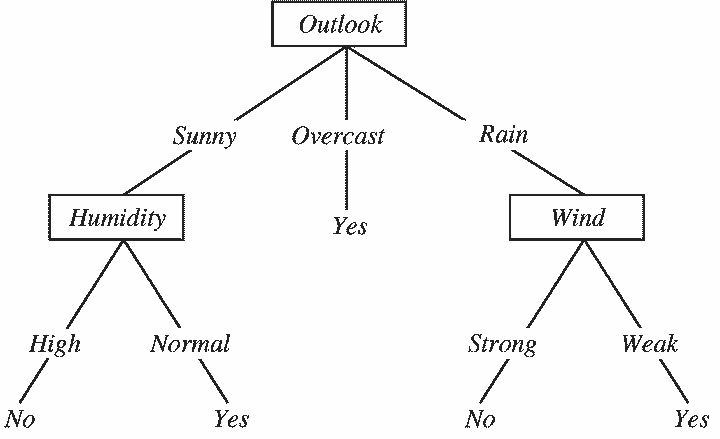
\includegraphics[width=.7\textwidth]{Figures/strom.png}
    \caption{Príklad rozhodovacieho stromu \cite{DecTreeTowards}}
    \label{pic:decTreeExample}
\end{figure}

Rozhodovacie stromy patria do triedy neparametrických supervised learning algoritmov, teda nie sú založené na matematickom modeli definujúcom vzťah medzi vstupom a výstupom ale učia sa z dát samotných. Vyznačujú sa vyššou flexibilitou ako parametrické algoritmy ale aj vyššou výpočtovou náročnosťou \cite{paramVSnonparam}. 

Existuje množstvo algoritmov pomocou ktorých je možné zostaviť rozhodovací strom zo vstupných dát. V tomto projekte sú využité algoritmy ID3, D4.5 a CART, ktorých popisu sú venované nasledujúce sekcie. 

\subsection{Algoritmus ID3}
\label{sec:ID3}
ID3, celým názvom Iterative Dichotomiser 3, je klasifikačný algoritmus publikovaný Rossom Quinlanom v roku 1975. ID3 vytvára rozhodovací strom zo vstupnej dátovej sady na základe miery Information Gain (IG). Nakoľko sa výpočet IG do veľkej miery opiera o pojem Entropia, sú obe tieto miery definované v nasledujúcom texte. 

Algoritmus na vstupe dostane dátovú sadu vo forme tabuľky, kde jednotlivé riadky je možné predstaviť si ako objekty a stĺpce ako atribúty týchto objektov. Jeden z týchto atribútov je označený ako cieľový a zostrojený rozhodovací strom bude na základe hodnôt zvyšných atribútov určovať jeho hodnotu. Algoritmus postupuje po iteráciách a v každej iterácií vyberie ne-cieľový atribút s najvyššou hodnotou IG, z ktorého sa stane koreň aktuálneho pod-stromu. Spojením všetkých takto vzniknutých pod-stromov vzniká celý rozhodovací strom \cite{hssina2014comparative}. Pseudokód algoritmu je možné vidieť na obrázku \ref{pic:id3Pseudo}.

\begin{figure}[!htb]
    \centering
    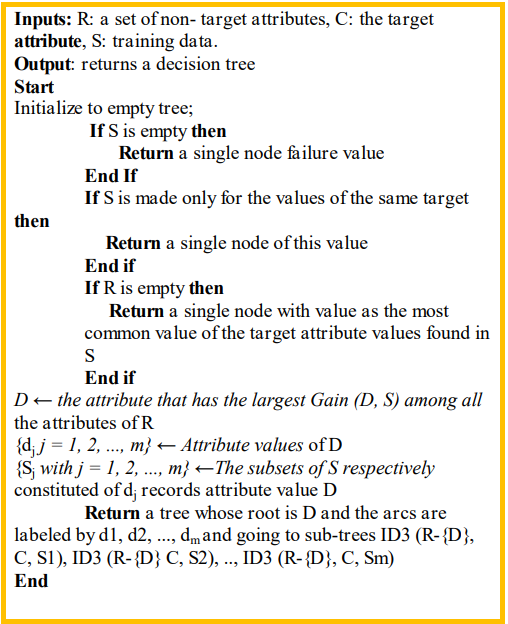
\includegraphics[width=.55\textwidth]{Figures/id3Pseudo.png}
    \caption{Pseudokód algoritmu ID3 \cite{hssina2014comparative}}
    \label{pic:id3Pseudo}
\end{figure}

\subsubsection*{Miery využívané algoritmom ID3}
\label{sec:ID3miery}
Entropia je miera v teórií informácií, ktorá vyjadruje neusporiadanosť (neurčitosť) v skupine pozorovaní \cite{EntropyAndGain}. Uvažujme dátovú sadu D s N rôznymi triedami objektov, kde P(\textit{i}) je pravdepodobnosť výberu triedy \textit{i}. Entropia tejto dátovej sady je potom daná vzorcom: 

\[Entropy(D) = -\displaystyle\sum\limits_{i=1}^n P(i) \times \log_2(P(i))\]

Information gain je možné charakterizovať ako mieru toho, koľko informácií o triede \textit{i} poskytuje atribút A, pomocou čoho je možné určiť poradie atribútov v rozhodovacom strome \cite{EntropyAndGain}. Gain atribútu A s N rôznymi triedami objektov je teda možné určiť ako:

\[Gain(A) = Entropy(D) - \displaystyle\sum\limits_{j=1}^n P(j) \times E(D_j)\]

kde \textit{j} reprezentuje triedu atribútu A a $D_j$ značí podmnožinu dátovej sady v ktorej všetky objekty spadajú do triedy \textit{j} podľa atribútu A.

\subsection{Algoritmus D4.5}
\label{sec:D45}
Algoritmus D4.5 bol publikovaný v roku 1993 Rossom Quinlanom ako rozšírenie algoritmu ID3 od rovnakého autora. Oba algoritmy sú si koncepčne veľmi podobné. Hlavnou výhodou algoritmu D4.5 oproti algoritmu ID3 je menšia citlivosť na atribúty s veľkým počtom hodnôt a je teda vhodnejší na tento typ vstupnej dátovej sady. Algoritmus D4.5 uprednostňuje pri vytváraní rozhodovacieho stromu atribúty s vyššou hodnotou miery Gain ratio, ktorej výpočet využíva miery Information Gain a Split Info \cite{hssina2014comparative}. Miera IG bola popísaná v predchádzajúcej sekcií v rámci popisu algoritmu ID3, zvyšné miery sú popísané v nasledujúcich odstavcoch.

\subsubsection*{Miery využívané algoritmom D4.5}
\label{sec:D45miery}
Mieru Gain Ratio je možné chápať ako normalizovanú hodnotu miery Information Gain \cite{hssina2014comparative}. Jej výpočet je daný vzorcom:

\[GainRatio(A) = \frac{Gain(A)}{SplitInfo(A)}\]

Miera Split Info určuje počet vetiev rozhodovacieho stromu, ktoré by vznikli pri rozdelení podľa daného atribútu. Je daná vzorcom:

\[SplitInfo(A) = - \displaystyle\sum\limits_{j=1}^n P(j) \times \log_2(P(j))\]

\subsection{Algoritmus CART}
\label{sec:CART}
Algoritmus CART, celým názvom Classification and Regression Tree podobne ako algoritmy ID3 a D4.5 vytvára rozhodovací strom zo vstupnej dátovej sady. Ako napovedá jeho názov je možné ho použiť na úlohy vyžadujúce klasifikáciu aj regresiu. Výstupom tohto algoritmu je vždy binárny rozhodovací strom, teda každý vrchol má najviac dvoch potomkov a s výnimkou koreňa práve jedného predka \cite{CART}. Princíp fungovania algoritmu je opäť veľmi podobný algoritmom ID3 a D4.5. Metrikou použitou pre posúdenie kvality rozdelenia je Gini Index.

Gini index vyjadruje pravdepodobnosť, že náhodne vybraný objekt bude nesprávne klasifikovaný podľa distribúcie tried v dátovej sade. Hodnota Gini indexu sa pohybuje na škále 0--1, kde 0 značí, že všetky objekty patria do jednej triedy alebo v dátovej sade existuje iba jedna trieda, 1 značí, že objekty sú náhodne rozložené medzi triedami a hodnota 0,5 značí rovnomerné rozloženie objektov \cite{Gini}. Výpočet je daný vzorcom:

\[Gini(A) = 1 - \displaystyle\sum\limits_{i=1}^n P(i)^2\]

\section{Reinforcement learning}
\label{sec:ReinfoOverview}
Ako už bolo spomenuté na začiatku tejto kapitoly, algoritmy strojového učenia spadajúce do triedy reinforcement learningu sa vyznačujú tým, že pracujú s agentom, ktorý je vložený do určitého prostredia a učenie prebieha na základe spätnej väzby. Agent nemá explicitne určené, čo je jeho cieľom. 

Formálne je možné proces popísať na základe Markovho rozhodovacieho procesu, ktorý umožňuje matematicky modelovať rozhodovací proces agenta v dynamickom prostredí. Tento model pracuje s pojmami agent, stav, akcia, odmena a policy. Po vykonaní určitej akcie \textit{A} v danom prostredí sa agent dostane do stavu \textit{S}. Agent dostáva spätnú väzbu vo forme odmeny \textit{R} na základe akcií, ktoré vykoná a stavu, do ktorého sa dostane. Policy určuje optimálnu akciu agenta na základe aktuálneho stavu s cieľom maximalizovať odmenu \cite{Markov}. Zápornú hodnotu odmeny je možné chápať ako trest. Opakovaním daného postupu potom agent upravuje svoj rozhodovací proces. Tento postup je znázornený na obrázku \ref{pic:reinfoPic}.
  
\begin{figure}[!htbp]
    \centering
    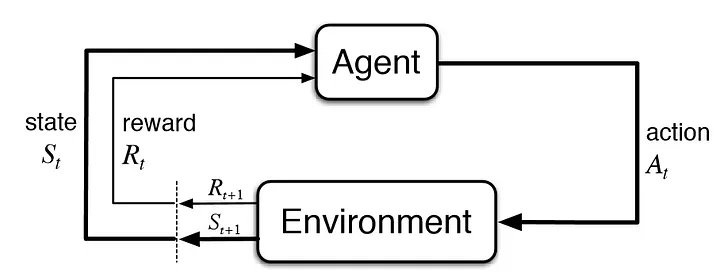
\includegraphics[width=.9\textwidth]{Figures/reinfoGraph.png}
    \caption{Princíp reinforcement learningu \cite{reinfoGraph}}
    \label{pic:reinfoPic}
\end{figure}

Algoritmy reinforcement learningu sú vhodné na aplikáciu v robotike, pri spracovaní prirodzeného jazyka, v samo-riadiacich autách apod. Reinforcement learning by mohol do budúcna priniesť zaujímavé výsledky aj v oblasti AI v počítačových hrách. V minulosti vznikli projekty v rámci ktorých dokázali agenti s využitím algoritmov reinforcement learningu hrať hry ako Go, StartCraft II či Dota 2 \cite{app13042443}. Vo veľkých komerčných projektoch sa však tieto algoritmy až na výnimky v podobe niektorých závodných hier veľmi nevyskytujú, a to aj napriek tomu, že principiálne má reinforcement learning blízko k rozhodovaniu NPC v hre. Časť tejto práce sa venuje práve problematike ich nasadenia v 3D hernom prostredí.

V tomto projekte bol ako zástupca triedy algoritmov reinforcement learningu zvolený algoritmus PPO, teda Proximal Policy Optimization, ktorý je bližšie popísaný v nasledujúcej sekcií.

%TODO - Pridaj nad aj pod zmienky o pripadnom dalsom algoritme ak sa podari

\subsection{Proximal Policy Optimization}
\label{sec:PPO}
Proximal Policy Optimization (PPO) je algoritmus reinforcement learningu, ktorý bol publikovaný v roku 2017 vedcami zo spoločnosti OpenAI. Hlavnými výhodami oproti jeho predchodcovi TRPO (Trust Region Policy Optimization) publikovanom v roku 2015 sú jednoduchšia implementácia, vyššia obecnosť a nižší nutný počet trénovacích vzoriek na naučenie cieľovej funkcie podľa empirického pozorovania \cite{PPOPaper}.

Pri supervised learningu je možné relatívne jednoducho implementovať cost funkciu a pomocou metódy gradient descent dosiahnuť dobrých výsledkov bez nutnosti náročného ladenia hyper-parametrov. Výsledky dosiahnuté pomocou algoritmov reinforcement learningu sú však veľmi citlivé na zmeny týchto parametrov. Algoritmus PPO sa snaží hľadať rovnováhu medzi zložitosťou implementácie, nutným počtom trénovacích vzoriek a práve ladením hyper-parametrov \cite{PPOPaper}.

Algoritmus PPO využíva tzv. policy gradient method \cite{PPOPaper}, čo znamená, že narozdiel napríklad od algoritmov Q-learningu sa agent neučí z uložených predchádzajúcich pokusov ale priamo na aktuálne vykonaných akciách v prostredí. Nevýhodou tohto typu algoritmov býva menšia efektivita využitia trénovacích vzoriek, nakoľko vzorky nie sú využité pri učení opakovane, a teda vyššie nároky na ich počet. Ako už však bolo spomenuté, túto nevýhodu sa PPO snaží minimalizovať.  

Algoritmus sa v každom kroku snaží minimalizovať cost funkciu pomocou malých odchýlok od predchádzajúcej policy. Maximálna veľkosť odchýlky je zabezpečená pomocou funkcie clip() v účelovej funkcií a dá sa ladiť pomocou hyper-parametru \(\varepsilon\) \cite{PPOPaper}. Účelová funkcia, ktorá sa typicky nevyskytuje v iných algoritmoch, je nasledovná:
\\\\
\[L^{CLIP}(\theta) = \hat{E}_t [min(r_t(\theta))\hat{A}_t, clip(r_t(\theta), 1 - \varepsilon, 1 + \varepsilon)\hat{A}_t]\]

kde:
\begin{itemize}
  \item \(\theta\) je parameter policy
  \item \(\hat{E}_t\) označuje empirické očakávanie v priebehu časového kroku
  \item \(r_t\) je pomer pravdepodobnosti podľa novej a starej policy
  \item \(\hat{A}_t\) je odhadovaná výhoda v čase \textit{t}
  \item \(\varepsilon\) je hyper-parameter, obecne nadobúda hodnotu v rozsahu 0,1--0,2
\end{itemize}

Účelová funkcia sa teda snaží optimalizovať očakávanie v priebehu časového kroku \(\hat{E}_t\). Hodnota \(\hat{E}_t\) je daná menšou z hodnôt \(r_t(\theta))\hat{A}_t\), čo je normálna policy, a jej variantou obmedzenou hyper-parametrom \(\varepsilon\). Toto obmedzenie zabraňuje veľkým zmenám od predchádzajúcej policy. Priebeh účelovej funkcie v závislosti od toho, či je odhadovaná výhoda kladná alebo záporná je možné vidieť na obrázku \ref{pic:clipping}.

\begin{figure}[!htbp]
    \centering
    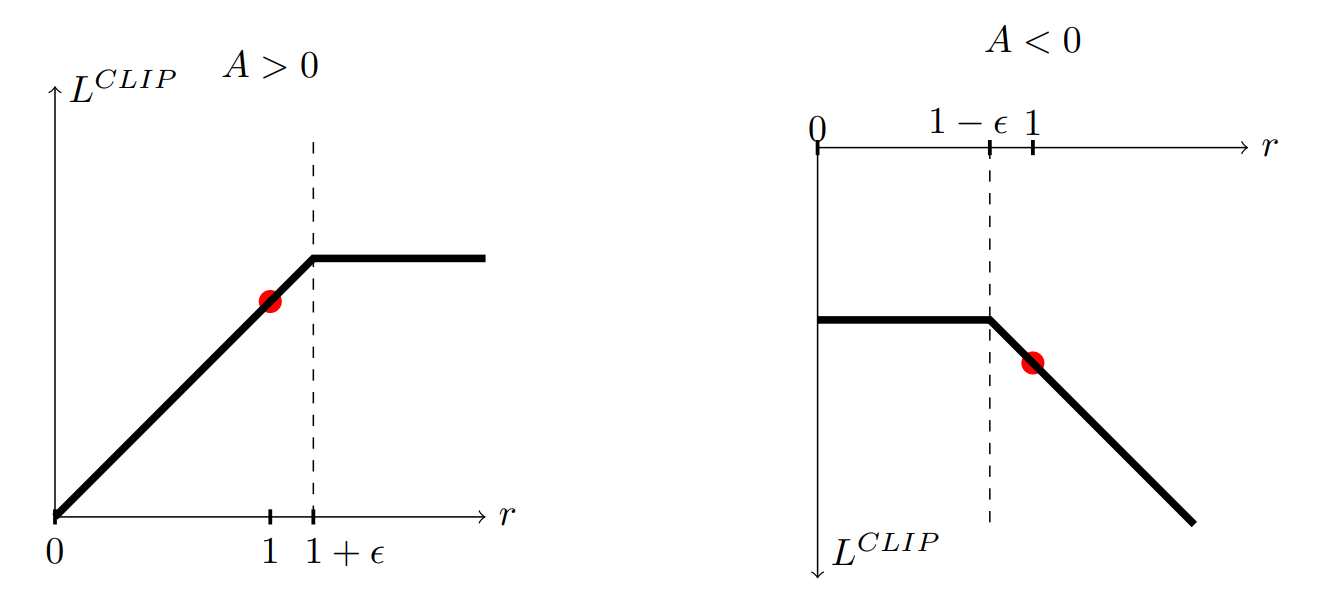
\includegraphics[width=.7\textwidth]{Figures/clip.png}
    \caption{Priebeh účelovej funkcie pre kladnú a zápornú odhadovanú výhodu \cite{PPOPaper}}
    \label{pic:clipping}
\end{figure}

% ------------------------------------------------------

% Vypracovanie
% Chapter 3
\chapter{Použité technológie}
\label{sec:Tech}
V tejto kapitole sú v stručnosti popísané najdôležitejšie technológie využívané pri tvorbe tohto projektu. Čast textu je zameraná aj na popis motivácie, ktorá viedla k využitiu daných technológií, ich výhody, nevýhody, prípadne zvažované alternatívy z hľadiska vhodnosti pre projekt celkovo, či jeho dielčie časti.

\section{Unity Engine}
\label{sec:Unity}
Unity je herný engine určený k tvorbe 2D a 3D interaktívneho obsahu renderovaného v reálnom čase. Od roku 2005 je vyvíjaný spoločnosťou Unity Technologies \cite{Unity}. Engine je vytvorený v programovacom jazyku C++, vývoj obsahu však prebieha v jazyku C\# či pomocou vizuálneho skriptovacieho nástroja Bolt vo forme rozšírenia od spoločnosti Unity Technologies. V posledných rokoch sa vývoj enginu Unity sústredí primárne na menšie hry a mobilný trh s dôrazom na monetizáciu mobilných hier pomocou mikro-transakcií a analytické nástroje pre vývojárov. Engine samotný však umožňuje tvorbu rôzneho druhu obsahu pre širokú škálu platforiem od herných konzolí cez desktopové operačné systémy až po VR, Microsoft HoloLens, AndroidTV či web vo forme WebGL \cite{UnityMultiplatform}. Engine Unity je možné využívať zdarma v rámci štúdia či pri malých projektoch, ktorých predaje nepresahujú čiastku \$100K za posledných 12 mesiacov \cite{UnityPersonal}.

Unity bol pri tvorbe tohto projektu zvolený z dôvodu predchádzajúcich skúseností, možnosti tvorby v programovacom jazyku C\#, množstvu dostupných materiálov a kvalite dokumentácie, ktorému sa v dobe písania tejto práce konkurencia hlavne v podobe enginu Unreal nemôže rovnať. Taktiež umožňuje rýchlejšiu tvorbu a prototypovanie ako väčšina konkurenčných nástrojov a rozsah projektu si nevyžadoval špeciálne technológie obsiahnuté napríklad v už spomínanom konkurenčnom engine Unreal ako Nanite, Lumen apod. Zároveň sa pomocou projektov ako ML-Agents či Perception čoraz viac stáva vyhľadávanou platformou v oblasti výskumu strojového učenia.

\section{Programovacie jazyky}
\label{sec:langs}
V tomto projekte sú využité dva programovacie jazyky. Hlavným jazykom je jazyk C\#, ktorý je využitý pri ovládaní hráčskej postavy, kamery, agentov, na detekciu interakcie s objektami atď. Druhým využitým jazykom je Python. V tomto jazyku sú naprogramované algoritmy ID4, C4.5 a CART popísané v sekcií \ref{sec:DecisionTreesOverview}. Toto rozdelenie bolo zvolené z dvoch dôvodov. Prvým je lepšia podpora knižníc v jazyku Python na spracovanie dátových rámcov. Druhým dôvodom bola snaha oddeliť spracovanie vstupných dát pre algoritmy od hlavnej aplikácie, aby nemusela opakovane prejsť buildom pri úprave či pridaní nového algoritmu. Človek, ktorý dizajnuje/upravuje chovanie NPC teda nemusí mať prístup k projektu, ale iba nahradí príslušné textové dokumenty v zložke s buildom hry. Nasledujúce sekcie sú venované krátkemu popisu týchto programovacích jazykov.

\subsection{Programovací jazyk C\#}
\label{sec:langsCShartp}
C\# je univerzálny vysoko-úrovňový multi-paradigmatický staticky typovaný programovací jazyk predstavený v roku 2000 spoločnosťou Microsoft. Od svojho predstavenia je jazyk C\# neustále vyvíjaný a obohacovaný o nové vlastnosti. Primárnou paradigmou C\# je objektovo orientované programovanie, poskytuje však množstvo vlastností funkcionálnych jazykov ako LISP či Haskell. Základná syntax C\# je podobná jazykom C, C++ a Java, tá je však obohatená o unikátne prvky ako LINQ, ktoré by sa dali pripodobniť skôr k jazyku SQL. C\# má integrovanú automatickú správu pamäte vykonávanú tzv. Garbage Collectorom \cite{DotNetBook}. Výhodou tejto správy je, že nekladie nároky na vývojára, aby pamäť ručne uvoľňoval, robí to však zároveň z jazyka C\# nie úplne najvhodnejšiu voľbu na určité výkonovo-orientované aplikácie, medzi ktoré patria aj moderné vysoko-rozpočtové herné tituly. Túto skutočnosť je však možné sčasti obísť metódami ako object pooling apod.

Spolu s jazykom C\# je nutné spomenúť aj .NET ekosystém, vyvíjaný priamo firmou Microsoft, ktorý poskytuje runtime prostredie CLR a širokú škálu knižníc či možností umožňujúcich pohodlné nasadenie C\# v rôznych webových, desktopových či cloudových aplikáciách \cite{DotNetBook}.

Engine Unity využíva v dobe písania tejto práce jazyk C\# vo verzií 9.0 a kompilátor Roslyn. Nie všetky vlastnosti jazyka C\# 9.0, ako napríklad kovariantné návratové typy sú však v Unity dostupné \cite{compiler}. To isté platí aj o knižniciach .NET ekosystému. Spoločnosť Unity odporúča využívať špecifikáciu .NET Standard, kde je zaručená najväčšia kompatibilita s rôznymi platformami. Podporovaná verzia .NET Standard potom závisí od verzie samotného enginu \cite{netUnity}. 

Jedným z posledných aspektov jazyka C\#, ktorý sa neodporúča využívať u potomkov triedy UnityEngine.Object sú operátory ?? a ?, nakoľko ich nie je možné overridnuť narozdieľ od operátorov == a !=. Dôvodom je, že po pokuse odstrániť tieto objekty z pamäte, sa síce okamžite odstránia v natívnom C++ kóde ale v jazyku C\# sa o to postará Garbage Collector až pri ďalšom cykle uvoľňovania pamäte. V čase medzi odstránením objektu z natívneho C++ kódu a manažovaného C\# kódu teda operátory ??, ? a ==, != vracajú nekonzistentné výsledky \cite{netUnity}.

\subsection{Programovací jazyk Python}
\label{sec:langsPython}
Python je podobne ako jazyk C\# vysoko-úrovňový multi-paradigmatický jazyk, ktorý je však dynamicky typovaný a čisto interpretovaný. Predstavený bol už v roku 1991, dodnes sa však teší veľkej popularite a podlieha kontinuálnemu vývoju. V dobe písania tejto práce má najaktuálnejšia verzia označenie 3.11. 

Vďaka strmej učebnej krivke a úspornej syntaxi je často využívaný pri výučbe programovania či prototypovaní. Okrem toho je ale veľmi využívaný v oblasti strojového učenia a dátovej analýzy, vo webovom vývoji či automatizácií rôznych úkonov. Obsahuje širokú škálu knižníc ako pandas, numpy, matplotlib či frameworkov ako Django, Flask, ktoré sú vytvárané komunitou alebo rôznymi spoločnosťami a robia tak z jazyka Python tak obľúbený nástroj. Nevýhodou jazyka je jeho výkon. Nakoľko interpretácia Python kódu je relatívne pomalá operácia, nemôže z tohto hľadiska konkurovať iným kompilovaným jazykom. Túto nevýhodu dokáže sčasti prekonať jeho dobrá integrácia s jazykmi C a C++, čo umožňuje vytvárať knižnice priamo v týchto jazykoch a tým optimalizovať kritické časti kódu či náročné matematické operácie \cite{pajton}.

\section{Nástroj ML-Agents}
\label{sec:ML-Agents}
ML-Agents \cite{mlagents} je open-source projekt, ktorý umožňuje využiť prostredie vytvorené v engine Unity na tréning agentov pomocou algoritmov reinforcement learningu ako PPO, SAC, MA-POCA a ďalších. Okrem reinforcement learningu obsahuje ML-Agents aj podporu pre algoritmy imitation learningu ako BC a GAIL, neuro-evolúciu apod. ML-Agents poskytuje implementáciu týchto algoritmov založenú na Python frameworku PyTorch spolu s medziprocesovou komunikáciu medzi enginom Unity a týmito algoritmami. Taktiež ponúka možnosť importu natrénovaných modelov naspäť do enginu, kde je možné na základe nich nechať agentov vykonávať rozhodnutia. Týchto agentov je možné trénovať či testovať v kontexte 2D, 3D či VR/AR hier a vedeckých simulácií. Okrem ovládania NPC je nástroj ML-Agents možné využiť aj v oblastiach ako automatizované testovanie apod.

Nástroj ML-Agents poskytuje množstvo komponentov na strane enginu Unity napísaných v jazyku C\#, ktoré je možné využiť či ďalej rozšíriť, aby vyhovovali potrebám takmer všetkých scenárov. Okrem toho však poskytuje aj Python API na tvorbu či úpravu trénovacích algoritmov, u ktorých je samozrejme možné ladiť rôzne hyper-parametre pomocou štruktúrovaných textových súborov. Taktiež je možné vizualizovať učebnú krivku agenta v podobe kumulatívnej odmeny, dĺžky trvania epizódy apod. pomocou nástroja TensorBoard.

ML-Agents je neustále vyvíjaný a jeho posledná stabilná verzia s označením 20 vyšla v novembri 2022. Medzi najväčšie limitácie patrí podpora buildu iba pre platformy Windows, Mac a Linux. Tá je však obmedzená iba na scripting backend Mono a teda nie je možné využiť IL2CPP \cite{mlagentsGit}. Oba tieto problémy sa však týkajú primárne väčších komerčných projektov a v tomto prípade neboli prekážkou.

Hlavným dôvodom pre výber tohto nástroja bola jeho otvorenosť a priama podpora enginu Unity z hľadiska poskytovaných komponentov, medziprocesovej komunikácie a následného nasadenia modelu. V prípade zvolenia iného riešenia či vlastnej implementácie by všetky tieto aspekty museli byť vytvorené na mieru. Bez kontinuálnej podpory, ktorú však nástroju ML-Agents poskytuje komunita, by takéto riešenie rýchlo prestalo byť funkčné v novších verziách enginu Unity.

\begin{figure}[!htbp]
    \centering
    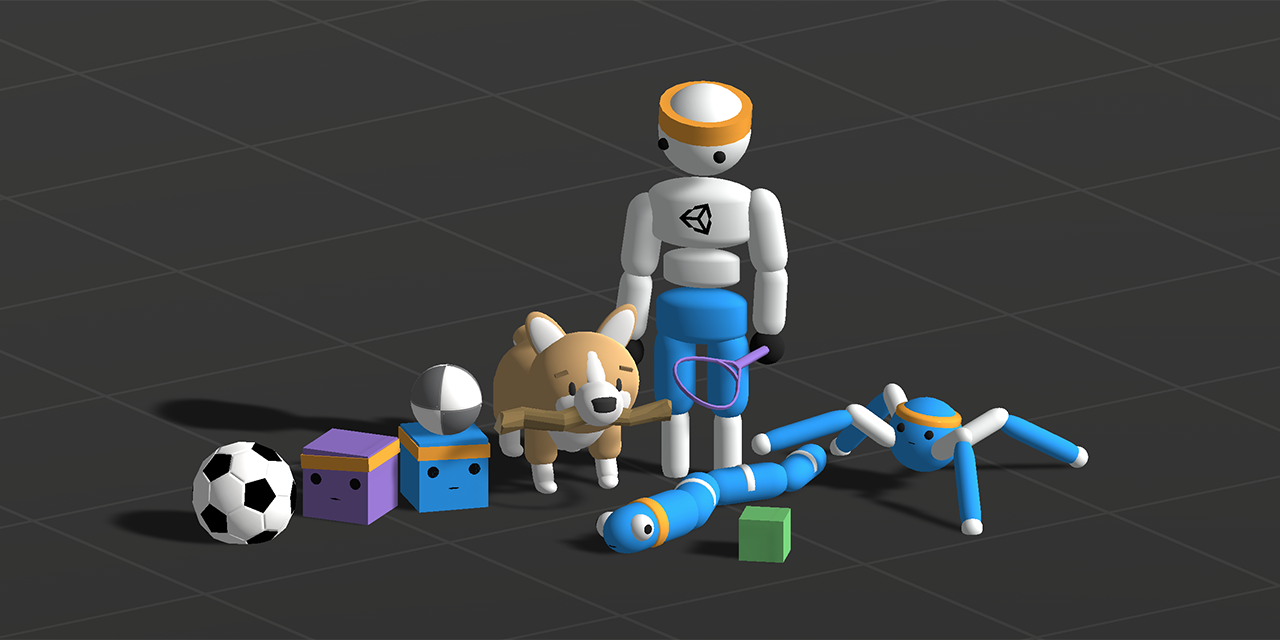
\includegraphics[width=.9\textwidth]{Figures/mlagents.png}
    \caption{Titulný obrázok nástroja ML-Agents \cite{mlagentsWeb}}
    \label{pic:mlagetnsLogo}
\end{figure}

\subsection{Inštalácia a prvotné nastavenie}
\label{sec:MLAgentsInstall}
Pre využitie nástroja ML-Agents je nutné mať nainštalovaný programovací jazyk Python. Podporovaná verzia jazyka sa líši v závislosti od konkrétneho releasu ML-Agents. V tomto projekte bol využitý ML-Agents v release 19 a Python vo verzií 3.9.13. Nakoľko je nástroj ML-Agents citlivý na verzie rôznych knižníc, bolo pre účel tohto projektu vytvorené uzavreté prostredie pomocou open-source distribúcie Anaconda. Tento krok však nie je povinný. Následne je nutné stiahnuť konkrétny release korešpondujúci s verziou enginu Unity z platformy GitHub, rozbaliť archív a v príkazovom riadku sa navigovať do rozbalenej zložky.

Ďalej je potrebné pomocou manažéra python balíkov pip spustiť nasledujúce príkazy:
\begin{itemize}
  \item pip3 install torch -f https://download.pytorch.org/whl/torch\_stable.html
  \item pip3 install -e ./ml-agents-envs
  \item pip3 install -e ./ml-agents
\end{itemize}

Prvý spomenutý príkaz sa pokúsi stiahnuť poslednú stabilnú distribúciu knižnice PyTorch. Tento krok však môže zlyhať kvôli rôznym problémom s kompatibilitou HW. V takomto prípade je nutné knižnicu stiahnuť ručne pomocou konfigurátoru na stránke PyTorch alebo v archíve distribúcií. Nakoľko sa verzie knižnice líšia aj v závislosti od modelovej rady procesoru nie je možné vytvorený Anaconda environment jednoducho distribuovať medzi zariadeniami. Zvyšné dva príkazy nainštalujú knižnice ml-agents-envs a ml-agents z lokálneho úložiska. Pri inštalácií záleží na poradí.

Následne je nutné vytvoriť projekt v engine Unity alebo použiť už existujúci, do ktorého je potrebné pridať rozšírenie ML-Agents. Podporovanú verziu enginu Unity pre konkrétny release ML-Agents je opäť možné nájsť v dokumentácií. V tejto práci bola využitá verzia 2022.2.0b12.

Pridanie rozšírenia ML-Agents do projektu prebieha nasledovne: 
\begin{itemize}
  \item V ponuke \textit{Window > Package Manager} kliknúť na ikonu + a z drop-down menu vybrať vybrať voľbu \textit{Add Package from disk}
  \item V následnom dialógu vybrať súbor \textit{package.json} v zložke \textit{com.unity.ml-agents}, ktorá sa nachádza medzi súbormi stiahnutými z platformy GitHub
\end{itemize}

Rozšírenie ML-Agents je možné stiahnuť aj z online repozitára ale v takomto prípade nie je zaručená úplná kompatibilita, takže tento spôsob nie je odporúčaný. Po úspešnom nainštalovaní je možné začať využívať komponenty v engine Unity a vytvoriť herné prostredie na trénovanie agentov samotných. Tento proces je bližšie popísaný v nasledujúcich kapitolách. 

Pre otestovanie funkčnosti a lepšiemu pochopeniu fungovania jednotlivých aspektov je vhodné zo stiahnutých súborov importovať do projektu vzorové trénovacie scenáre. Niektoré z týchto scenárov však vyžadujú tzv. New Input System. Pre jeho aktiváciu v projekte je potrebné nastaviť možnosť \textit{Active Input Handling} v ponuke \textit{Edit > Project Settings > Player > Other Settings} na hodnotu \textit{Both} alebo \textit{Input System Package (New)}. V projektoch, ktoré využívajú inú ako tzv. build-in render pipeline je potrebné k dosiahnutiu plnej funkčnosti týchto vzorových trénovacích scenárov skonvertovať shadery. Tento postup závisí od využívanej pipeliny a niektoré shadery vytvorené na mieru musia byť upravené či nahradené úplne. Popis tohto postupu je však nad rámec tohto projektu.

% Chapter 4
\chapter{Hra a herné prostredie}
\label{sec:GameOverview}
Táto kapitola je venovaná vytvorenej hre ako takej, všetkým jej aspektom a princípom fungovania. Prvá sekcia si kladie za cieľ popísať žánrové a príbehové zasadenie hry. V ďalších sekciách je potom podrobne prebratá architektúra a fungovanie jednotlivých herných mechaník.

\begin{figure}[!htbp]
    \centering
    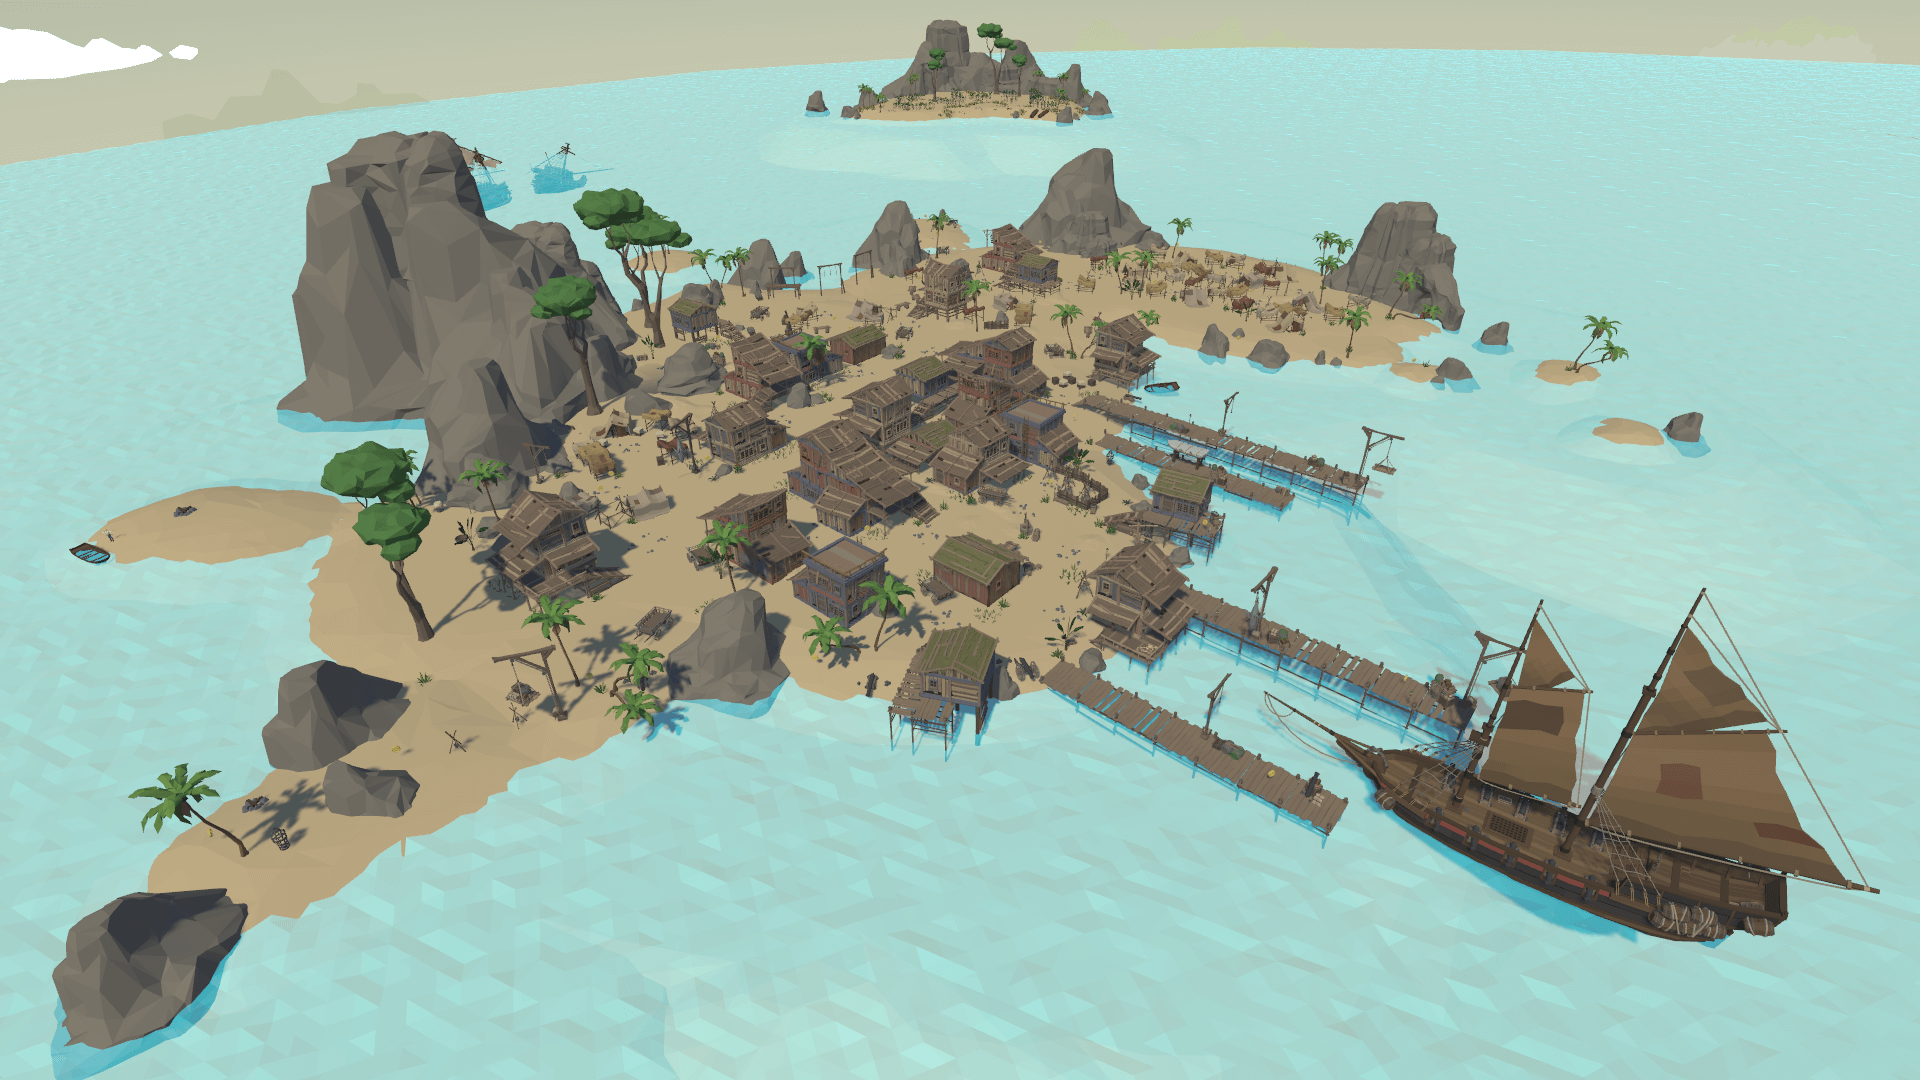
\includegraphics[width=.9\textwidth]{Figures/game_compressed.png}
    \caption{Herné prostredie}
    \label{pic:GameScreenshot}
\end{figure}

\section{Žáner a príbehové zasadenie}
\label{sec:GenreAndSetting}
Hra samotná má svojou hrateľnosťou najbližšie k žánru stealth. Tento žáner sa vyznačuje tým, že hráč sa snaží vyhnúť odhaleniu a následnému priamemu stretu s nepriateľom. K dosiahnutiu cieľa je teda využívaný pomalý a tichý postup, kde každý krok by mal byť dobre premyslený a načasovaný. 

Príbeh hry je zasadený do pirátskeho prostredia. Hráč sa ocitá v roli radového člena pirátskej posádky, ktorá bola napadnutá flotilou anglického námorníctva. S vypätím všetkých síl sa mu na poškodenom záchrannom člne podarilo dostať na najbližší obývaný ostrov, kde však zisťuje, že tam niečo nie je v poriadku. Namiesto obyvateľov ostrova nachádza len agresívnych kostlivcov. 

Hráč ovláda postavu z pohľadu tretej osoby a jeho úlohou je nájsť na ostrove funkčný čln, pozbierať zásoby nutné na ďalšiu plavbu a pokiaľ možno pri tom nevzbudiť pozornosť.

\section{Architektúra hry}
\label{sec:GameStructure}
Hra je rozdelená do dvoch samostatných scén. Konkrétne ide o hlavnú scénu, kde sa odohráva samotná herná slučka a scénu s hlavnou ponukou. V engine Unity je možné medzi nimi ľubovoľne prepínať, prípadne ich mať aktívnych niekoľko naraz. Každá scéna, ktorá je zahrnutá v builde má pridelené poradové číslo, tzv. build index, ktorý slúži aj ako jednoznačný identifikátor. Scéna s build indexom nula je potom spustená hneď po štarte aplikácie.

Scénu je možné chápať ako koreňový adresár pre hierarchiu objektov v hre. Jednotlivé herné objekty je možné do nej vložiť priamo, alebo ako potomka iného herného objektu. Manipulácia s pozíciou, rotáciou či mierkou objektu sa teda aplikuje aj na všetkých jeho potomkov. Naopak to však neplatí. Z tohto dôvodu sa rozlišujú dve súradnicové sústavy, a síce globálna (celková) a lokálna (relatívna voči predkovi). Využitie globálnej súradnicovej sústavy však vyžaduje vziať do úvahy parametre všetkých predkov daného objektu v scéne, čo nie je ideálne z hľadiska výkonu. Preto bol v projekte preferovaný lokálny súradnicový systém napríklad u herných NPC agentov či predmetov, ktoré je v hre možné zbierať. Predkovia týchto objektov sú potom umiestnení v počiatku súradnicovej sústavy, čo zaisťuje konzistenciu so zvyškom objektov v scéne.

V každej scéne sa nachádza objekt MainManager, ktorý slúži ako prístupový bod k ostatným manažérom, ktorí spravujú centrálne prvky hry. Tento typ architektúry sa kvôli svojej jednoduchosti často uplatňuje medzi malými až strednými projektami. V tomto projekte sú použité objekty ConfigManager, GameManager, InputManager a SoundManager, nie všetky sú však vyžadované v každej scéne. 

Krátky popis jednotlivých manažérov:
\begin{itemize}
  \item \textbf{ConfigManager} -- je prístupovým bodom k nastaveniam hry a zaisťuje serializáciu či deserializáciu dát, rovnako ako ich perzistentnosť po každej zmene.
  \item \textbf{GameManager} -- reštartuje scénu pri smrti alebo výhre hráča, kontroluje prerekvizity výhry, aktualizuje grafické užívateľské rozhranie pri získaní predmetu a zobrazuje kontextovú ponuku na ukončenie hry či pre návrat do hlavnej ponuky po stlačení príslušnej klávesy.
  \item \textbf{InputManager} -- centralizuje získavanie užívateľského vstupu z klávesnice, myši, či iných herných periférií, čo umožňuje na jednom centrálnom mieste zamieňať rôzne implementácie, prípadne z testovacích dôvodov hráčsky vstup úplne ignorovať. 
  \item \textbf{SoundManager} -- vyvoláva jednoduchú simuláciu zvuku, na ktorú môžu zareagovať NPC agenti v dosahu.
\end{itemize}

\section{Herná slučka}
\label{sec:GameLoop}
Tradičná herná slučka definovaná napríklad podľa \cite{GameAlgorithms} sa skladá z troch fáz:

\begin{enumerate}
  \item Spracovanie vstupov
  \item Aktualizácia herného sveta
  \item Generovanie výstupov
\end{enumerate}

Hra teda prijme užívateľský vstup, aktualizuje herný svet resp.dynamické objekty, ktoré sa v ňom vyskytujú a výsledný stav je potom vyrenderovaný hráčovi v ďalšom snímku. Tento postup sa opakuje niekoľkokrát za sekundu, čo vyvoláva ilúziu dynamického sveta. Dnes sa považuje za štandard vykonanie hernej slučky 30 až 60 krát za sekundu. Moderný hardvér však už podporuje vykresľovanie aj o rýchlosti 500FPS. Lepšou metrikou pre vývojárov je však tzv. frame time, teda trvanie jednej hernej slučky v ms. Vzťah týchto veličín je znázornený na obrázku \ref{pic:FrameTimeFPS}.

\begin{figure}[!htbp]
    \centering
    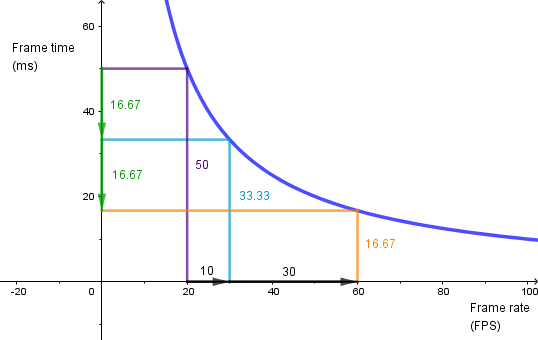
\includegraphics[width=.8\textwidth]{Figures/frameTimeVsFPS.png}
    \caption{Metriky Frame Time a FPS \cite{FrameTimeFPS}}
    \label{pic:FrameTimeFPS}
\end{figure}

V kontexte konkrétnej hry sa však pojem herná slučka alebo základná herná slučka (core game loop) využíva skôr na popis základných herných mechaník. V tomto prípade by teda šlo o prechod z bodu A do bodu B a zozbieranie určitého počtu predmetov na vymedzenej hernej ploche.

Pokiaľ hráčovi klesne život na nulu, hra pre neho končí a vracia sa na počiatočnú lokáciu. Nepriatelia a zberateľné predmety sa vrátia na svoje počiatočné pozície. Ak hráč dôjde do cieľa a splní prerekvizitu výhry, teda má v inventári určitý počet predmetov daného typu, hru vyhráva. Základnú hernú slučku obstaráva objekt GameManager spomenutý v sekcií \ref{sec:GameStructure}. 

Po hernej ploche je ručne rozmiestnených päť fliaš, z ktorých musí hráč nájsť a zobrať aspoň tri a tridsaťpäť mincí, pričom je pre dosiahnutie výhry nutné mať aspoň dvadsaťpäť. Implementačne oba typy objektov dedia z triedy Pickup, ktorej telo je možné vidieť vo výpise \ref{src:Pickup}. Tá potom dedí priamo z triedy UnityEngine.MonoBehaviour, čo je bázová trieda, z ktorej musia dediť všetky triedy, ktoré sú považované za Unity skripty. Unity skript môže potom využívať metódy životného cyklu ako napríklad Awake(), Start(), Update(), či FixedUpdate(), ale aj metódy sprístupňujúce prácu s korutinami apod. \cite{MonoBehaviour}.
\vspace{8pt}
\begin{lstlisting}[label=src:Pickup,caption={Trieda Pickup slúžiaca ako predok všetkých zberateľných predmetov v hre}]
public class Pickup : MonoBehaviour
{
    public event Action<Pickup> OnPickedUp;
    private WaitForEndOfFrame waitForFrameToEnd = new WaitForEndOfFrame();
    private MeshRenderer mesh;

    private void Start() 
    {
        MainManager.Instance.GameManager.RegisterPickup(this);
        mesh = GetComponentInChildren<MeshRenderer>();
    }
    
    private void OnTriggerEnter(Collider other) 
    {
        if (!other.gameObject.CompareTag(Constants.PlayerTag)) 
            return;

        OnPickedUp?.Invoke(this);
        StartCoroutine(LerpPosition(transform.position, Camera.Instance.PickupTarget.position, 0.2f, () => { gameObject.SetActive(false); }));
    }
    
    private void OnDestroy() 
    {
        MainManager.Instance.GameManager.UnregisterPickup(this);
    }
    
    IEnumerator LerpPosition(Vector3 start, Vector3 end, float timeToMove, Action callback) 
    {
        float time = 0;

        while (time < 1)
        {
            mesh.transform.position = Vector3.Lerp(start, end, time);
            time += Time.deltaTime / timeToMove;

            yield return waitForFrameToEnd;
        }

        mesh.transform.position = end;
        callback();
    }
}
\end{lstlisting}

V metóde Start(), teda na začiatku svojho životného cyklu, ktorý sa odohrá po spustení scény sa každý zberateľný objekt zaregistruje v objekte GameManager, čo spôsobí napojenie na event OnPickedUp a umožní GameManagerovi v správnej chvíli zareagovať na získanie predmetu hráčom a aktualizovať GUI či inventár bez nutnosti periodického dopytovania. Nakoľko je odberateľovi eventu odosielaná aj daná inštancia objektu, je jednoduché zistiť typ predmetu, ktorý hráč zobral.

Metóda OnTriggerEnter() je potom zavolaná v momente, keď hráčov kontroler začne kolidovať s komponentou Box Collider daného objektu. K tomu je nutné nastaviť tento Box Collider ako tzv. trigger a zároveň mať na objekte prítomnú komponentu Rigidbody, ktorá obstaráva simuláciu fyziky. V tomto momente sa zároveň pomocou korutiny LerpPosition() začne objekt rýchlo pohybovať do pravého horného rohu obrazovky, kde sa nachádza GUI element zobrazujúci hráčovi počet zozbieraných predmetov, a následne sa deaktivuje. Tento efekt bol často využívaný v starších 2D platformových hrách. Zberateľný predmet je možné vidieť na obrázku \ref{pic:Pickup}.

\begin{figure}[!htbp]
    \centering
    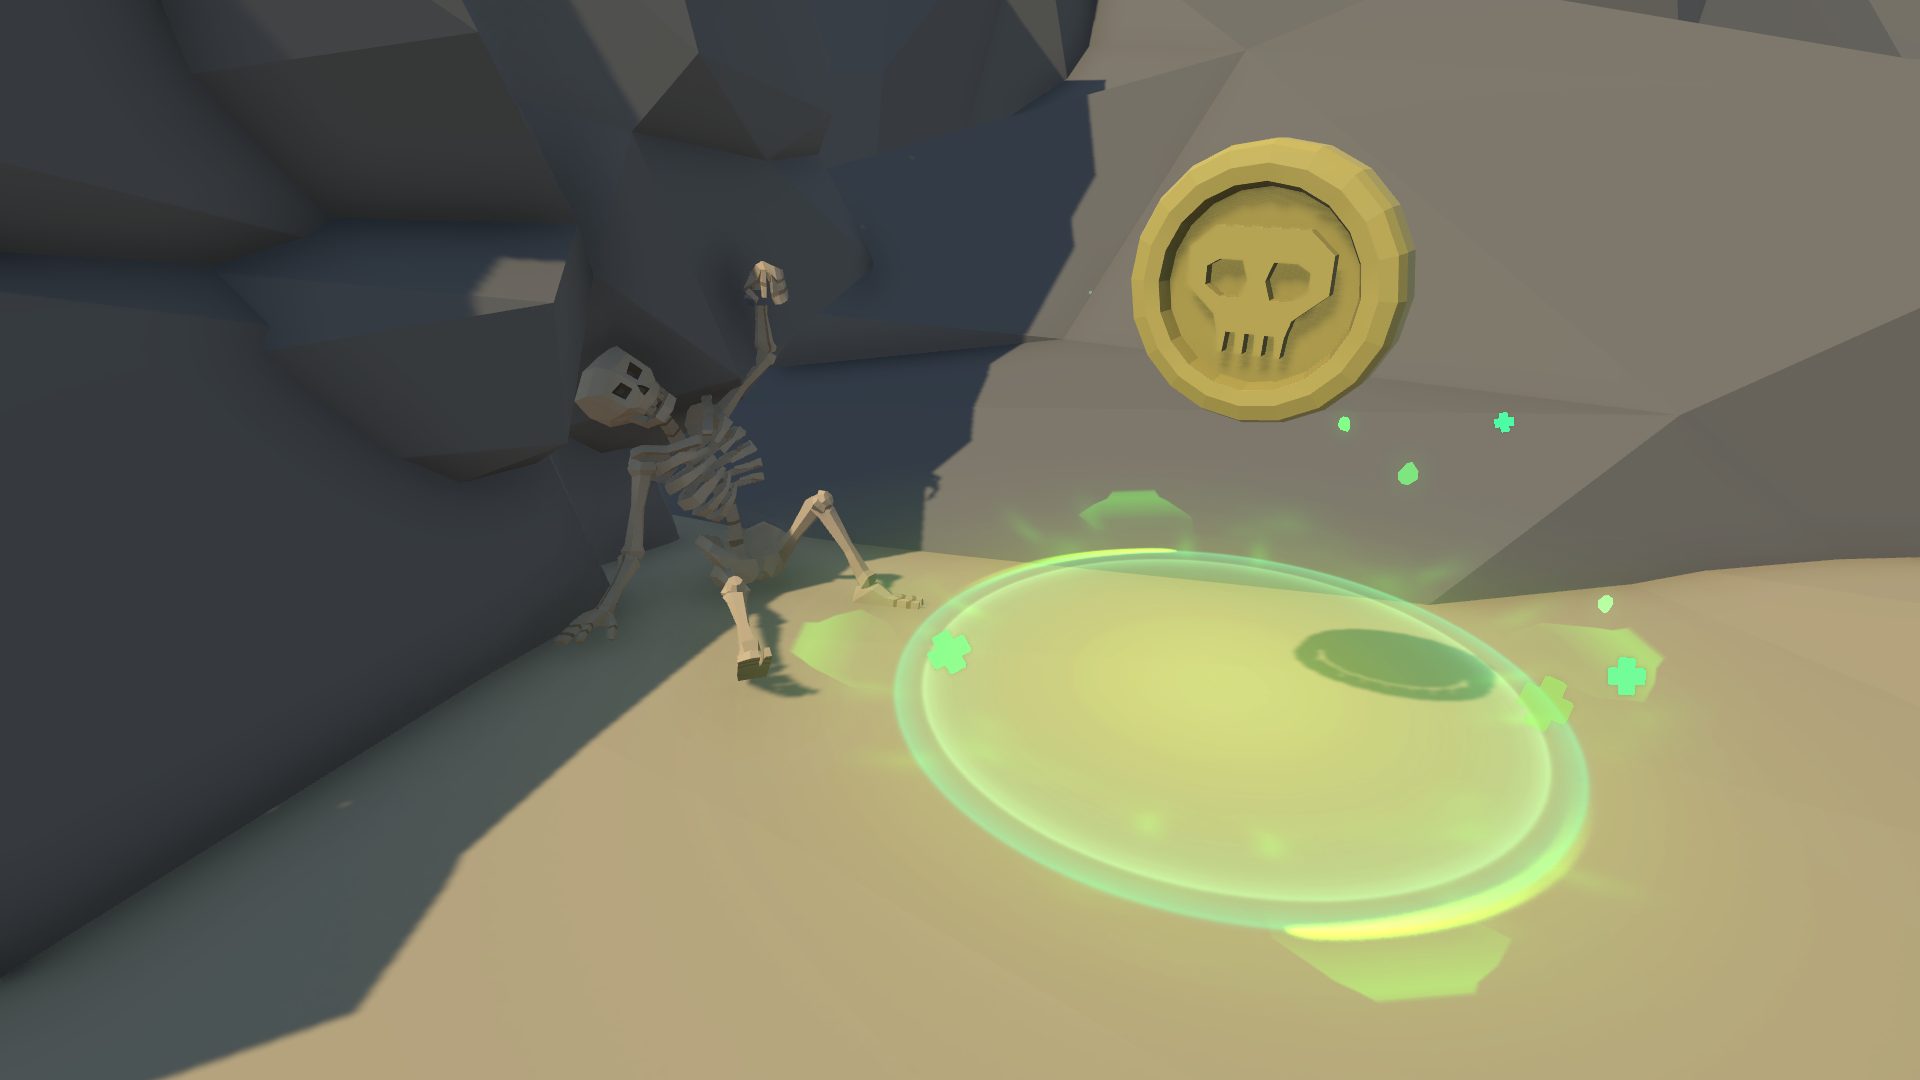
\includegraphics[width=.8\textwidth]{Figures/pickup.png}
    \caption{Zberateľný predmet minca}
    \label{pic:Pickup}
\end{figure}

Podobným spôsobom ako pri zberateľných predmetoch bola v projekte riešená aj interakcia s objektom Finish, ktorého úlohou je ukončiť hru v prípade, že s ním hráčov kontroler začne kolidovať. Taktiež teda obsahuje komponentu Box Collider nastavenú ako trigger a komponentu Rigidbody. Pri štarte hry sa tento Finish rovnako ako zberateľné predmety zaregistruje pod objekt GameManager a v metóde \mbox{OnTriggerEnter()}, po overení, že naozaj koliduje s hráčom, vyvolá event \mbox{OnTriggered}. 

Nakoľko bol Finish využívaný aj v trénovacej fáze, bol pre tento účel vytvorený jednoduchý interface IFinish obsahujúci spomínanú metódu OnTriggered a jeho dve implementácie: FinishGame a FinshEpisode. Prvá implementácia je využívaná v hlavnej scéne a ukončuje hru, druhá, ako názov napovedá, ukončuje trénovaciu epizódu v neprospech AI agenta. Táto problematika je bližšie popísaná v kapitole \ref{sec:Training}.

Po vyvolaní spomínaného eventu objekt GameManager overí prerekvizity výhry a pokiaľ ich hráč spĺňa, ukončí hru. Tento postup je možné vidieť vo výpise \ref{src:FinishGame}. Pomocou eventu OnGameFinished zároveň všetkým odberateľom oznámi ukončenie hry. Najdôležitejší odberatelia eventu sú herná kamera a pohybový systém hráča, ktorí okamžite zastavia svoju činnosť a stanú sa pasívnymi. Zároveň s týmto sa hráčovi začne postupne zobrazovať informácia o úspešnom dokončení hry a po určitej dobe sa reštartuje scéna, čo umožní hráčovi skúsiť to znova napríklad s inými parametrami.

\vspace{8pt}
\begin{lstlisting}[label=src:FinishGame,caption={Ukončenie hry v prípade výhry hráča}]
private bool PrerequisitesMet()
{
    return (pickedBottles >= minBottles) && (pickedCoins >= minCoins);
}
private void GameFinished()
{
    if (!PrerequisitesMet())
    {
        ShowPrerequisitesNotMetInfo();
        return;
    }

    OnGameFinished?.Invoke();

    if (youWonUI != null)
        youWonUI.SetActive(true);

    StartCoroutine(RestartSceneCoroutine());
}
private IEnumerator RestartSceneCoroutine()
{
    yield return uiWait;
    SceneManager.LoadScene(SceneManager.GetActiveScene().name);
}
\end{lstlisting}

Medzi ďalšie kompetencie GameManagera patrí inštancovanie NPC agentov určeného typu pri štarte hry na základe nastavení uložených v objekte ConfigManager. Bližší popis štruktúry agentov, ich inštancovanie a fungovanie je popísané v kapitole \ref{sec:Agents}.

Poslednou kompetenciou GameManagera je periodicky v rámci metódy OnUpdate() zisťovať od objektu InputManager, či bola stlačená klávesa na pozastavenie hry a na základe toho zobraziť hráčovi príslušný GUI element. Tento postup bol zvolený z dôvodu, že vstavaný input systém enginu Unity nedokáže spracovávať užívateľský vstup tzv. event-driven prístupom. Spomínaný GUI element je možné vidieť na obrázku \ref{pic:PauseUI} a umožňuje hráčovi rozhodnúť, či chce ukončiť hru alebo sa vrátiť do hlavnej ponuky. 

\begin{figure}[!htbp]
    \centering
    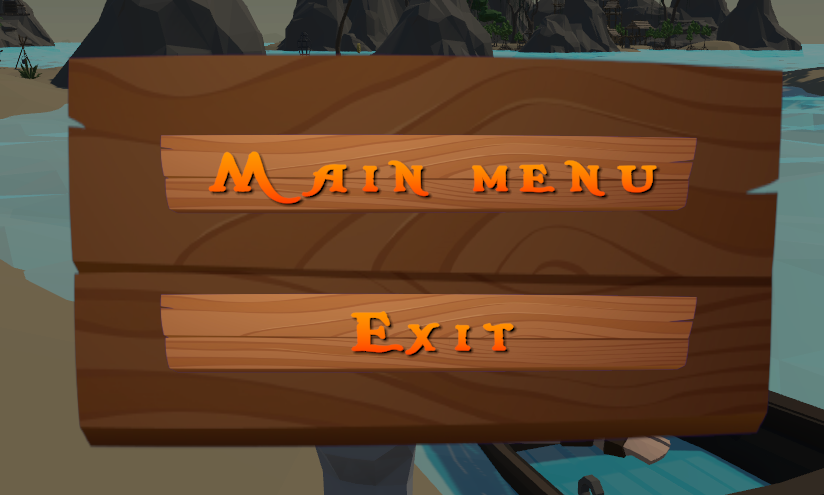
\includegraphics[width=.65\textwidth]{Figures/pauseUI.png}
    \caption{GUI element s umožňujúci návrat do hlavnej ponuky alebo ukončenie hry}
    \label{pic:PauseUI}
\end{figure}

Obe tlačidlá na GUI elemente zobrazenom na obrázku \ref{pic:PauseUI} obsahujú Unity komponentu Button, ktorá vie napríklad zmeniť farebnú schému elementu, keď nad ním hráč nadíde myšou. Dôležitejšou funkcionalitou je však možnosť priradiť eventu OnClick ľubovoľný objekt priamo v editore a nastaviť, že interakcia s tlačidlom bude na tomto objekte volať určenú verejnú metódu, čo demonštruje obrázok \ref{pic:OnClick}. 

\begin{figure}[!htbp]
    \centering
    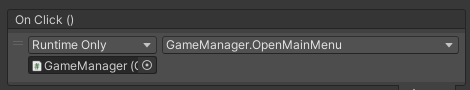
\includegraphics[width=.8\textwidth]{Figures/OnClick.png}
    \caption{Nastavenie OnClick eventu tlačidla v editore}
    \label{pic:OnClick}
\end{figure}

V tomto prípade bol tlačidlám predaný objekt GameManager a volané boli jeho dve verejné metódy OpenMainMenu() a QuitGame() zobrazené vo výpise \ref{src:MMQuit}.

\vspace{8pt}
\begin{lstlisting}[label=src:MMQuit,caption={Návrat do hlavnej ponuky a ukončenie hry}]
public void OpenMainMenu()
{
    SceneManager.LoadScene(0);
}
public void QuitGame()
{
#if UNITY_EDITOR
    UnityEditor.EditorApplication.isPlaying = false;
#endif
    Application.Quit();
}
\end{lstlisting}

Metóda OpenMainMenu() načíta scénu s build indexom nula. Tento postup je vhodné aplikovať pri fixne danom poradí scén. Zamedzí sa tým zbytočnému hľadaniu scény podľa jej mena. Poradie scén v rámci tohto projektu je popísané v sekcií \ref{sec:GameStructure}. 

Ukončenie hry potom prebieha jednoduchým zavolaním metódy Application.Quit(). Tento prístup však nefunguje na aplikáciu spustenú v editore Unity. Z tohto dôvodu je v rámci direktivy preprocesoru UNITY\_EDITOR, nutné aj nastavenie premennej isPlaying v triede UnityEditor.EditorApplication na hodnotu false. 

Direktívy preprocesoru v jazyku C\# umožňujú selektívne zahrnúť alebo vylúčiť kód z kompilácie na základe toho, či sú alebo nie sú definované určité skriptovacie symboly. Engine Unity ná na tieto účely preddefinované symboly umožňujúce rozlíšiť rôzne platformy či práve buildu aplikácie od behu v editore \cite{ConditionalCompilation}.

\section{Hlavná ponuka hry}
\label{sec:MainMenuAndUI}

Ako už bolo spomenuté v predchádzajúcich sekciách, vytvorená hra obsahuje scénu s hlavnou ponukou. Táto scéna obsahuje informačnú tabuľu s aktuálnymi nastaveniami a štyri aktívne prvky užívateľského rozhrania. Ide o tlačidlá Play, Options, Credits a Exit. Tieto tlačidlá opäť obsahujú Unity komponentu Button a referenciu na objekt, ktorého verejné metódy sú pri interakcii s tlačidlom volané. Hlavnú ponuku je možné vidieť na obrázku \ref{pic:MainMenu}.

\begin{figure}[!htbp]
    \centering
    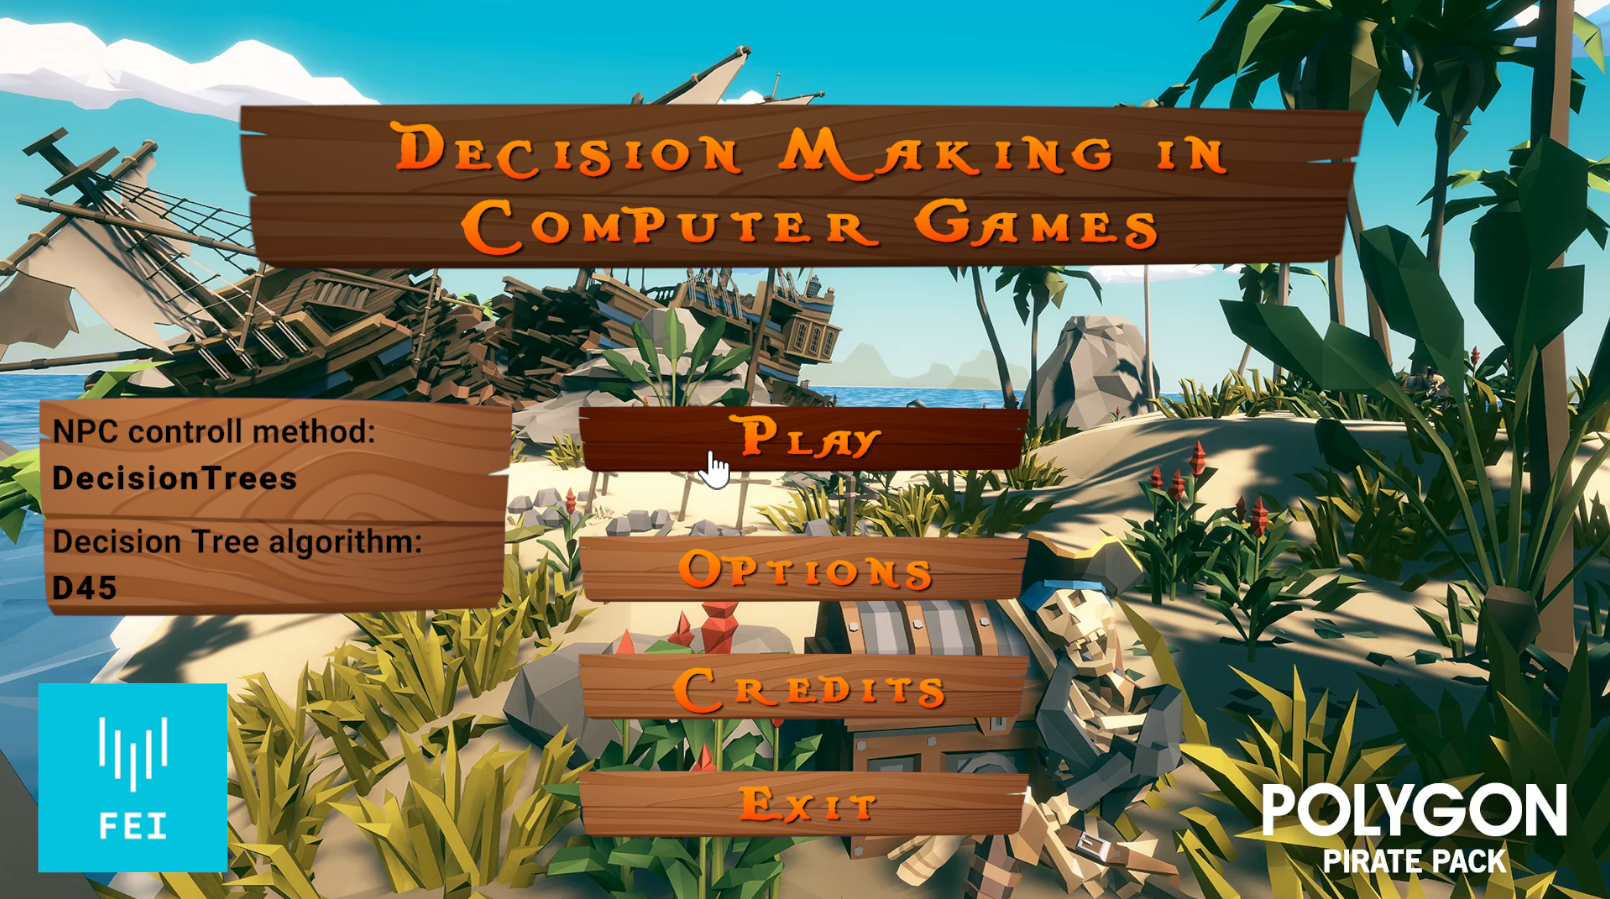
\includegraphics[width=.9\textwidth]{Figures/mainMenu.png}
    \caption{Hlavná ponuka hry}
    \label{pic:MainMenu}
\end{figure}

Informačná tabuľa na ľavej strane obrazovky zobrazuje, či budú NPC agenti v hre ovládaní rozhodovacím stromom alebo pomocou reinforcement learningu. Pokiaľ budú agenti ovládaní pomocou rozhodovacieho stromu, v spodnej časti tabule sa zobrazí aj algoritmus, ktorým má byť strom zostrojený. Tieto nastavenia sú perzistentné a teda ostanú uchované aj po vypnutí aplikácie. Zmeny je možné vykonať v ponuke Options, kde stlačenie príslušného tlačidla vyvolá zmenu na objekte ConfigManager. Ten pomocou jednoduchej metódy Serialize() tieto zmeny aktualizuje na disku v súbore \textit{settings.txt} uloženom v adresári, ktorého presné umiestnenie je dané premennou \textit{Application.persistentDataPath}. Konkrétna cesta sa teda líši v závislosti od aktuálnej platformy. Zároveň je zmena v dátach propagovaná pomocou eventu OnDataChanged, ktorého odberateľom je hlavná ponuka, ktorá tieto zmeny aktualizuje v informačnej tabuli.

Tlačidlo Exit ukončí beh aplikácie a tlačidlo Play spustí hlavnú scénu hry. Obdobná funkcionalita bola demonštrovaná už vo výpise \ref{src:MMQuit}.

Tlačidlo Credits zavolá na svojom predkovi v scéne metódu SetActive() so vstupným parametrom nastaveným na false. Tento predok združuje všetky tlačidlá, informačnú tabuľu a tabuľu s menom aktuálnej ponuky. Zároveň obdobným spôsobom aktivuje ponuku Credits, ktorá mu bola referencovaná v editore. 

Tlačidlo Options potom využíva rovnaký prístup na zobrazenie ponuky s výberom typu NPC agenta proti ktorému chce hráč hrať. V prípade, že hráč vyberie možnosť Decision Trees je mu ešte zobrazená ponuka s výberom algoritmu, ktorý chce použiť na zostavenie rozhodovacieho stromu.

Každá vnorená ponuka, ktorá sa stane aktívna sa začne periodicky dopytovať objektu InputManager, či bola stlačená príslušná klávesa na návrat do predchádzajúcej ponuky. Na tento účel bola vytvorená jednoduchá trieda zobrazená vo výpise \ref{src:SubMenu}.

\vspace{8pt}
\begin{lstlisting}[label=src:SubMenu,caption={Trieda SubMenu reprezentujúca vnorenú ponuku}]
public class SubMenu : MonoBehaviour
{
    [SerializeField]
    private GameObject currentSubMenu;
    [SerializeField]
    private GameObject previousSubMenu;

    private void Update()
    {
        if (MainManager.Instance.InputManager.WasCancelledLastFrame)
        {
            currentSubMenu.SetActive(false);
            previousSubMenu.SetActive(true);
        }
    }
}
\end{lstlisting}

Jednotlivé ponuky sú v triede referencované pomocou atribútu \textit{SerializeField} a na jednotlivých objektoch boli nastavené ručne v editore. Atribút \textit{SerializeField} vynúti serializáciu u neverejných členských premenných \cite{SerializeField}, čím sa neporušuje princíp zapuzdrenia a zároveň to umožňuje jednoducho referencovať medzi sebou objekty priamo v editore Unity pomocou tzv. drag \& drop či výberu z drop-down ponuky. Nie je teda nutné prehľadávať objekty v scéne alebo riešiť prístup k danému objektu architektonicky na úrovni kódu. Tento prístup však nie je možné použiť na prepojenie dvoch objektov, pričom jeden z nich je prítomný v scéne od začiatku a druhý je inštancovaný za behu aplikácie. Všetky jednotlivé ponuky sú súčasťou hierarchie scény od jej spustenia, takže nebol s týmto prístupom problém. Diagram všetkých ponúk je možné vidieť na obrázku \ref{pic:MainMenuScheme}.

\begin{figure}[!htbp]
	\centering
	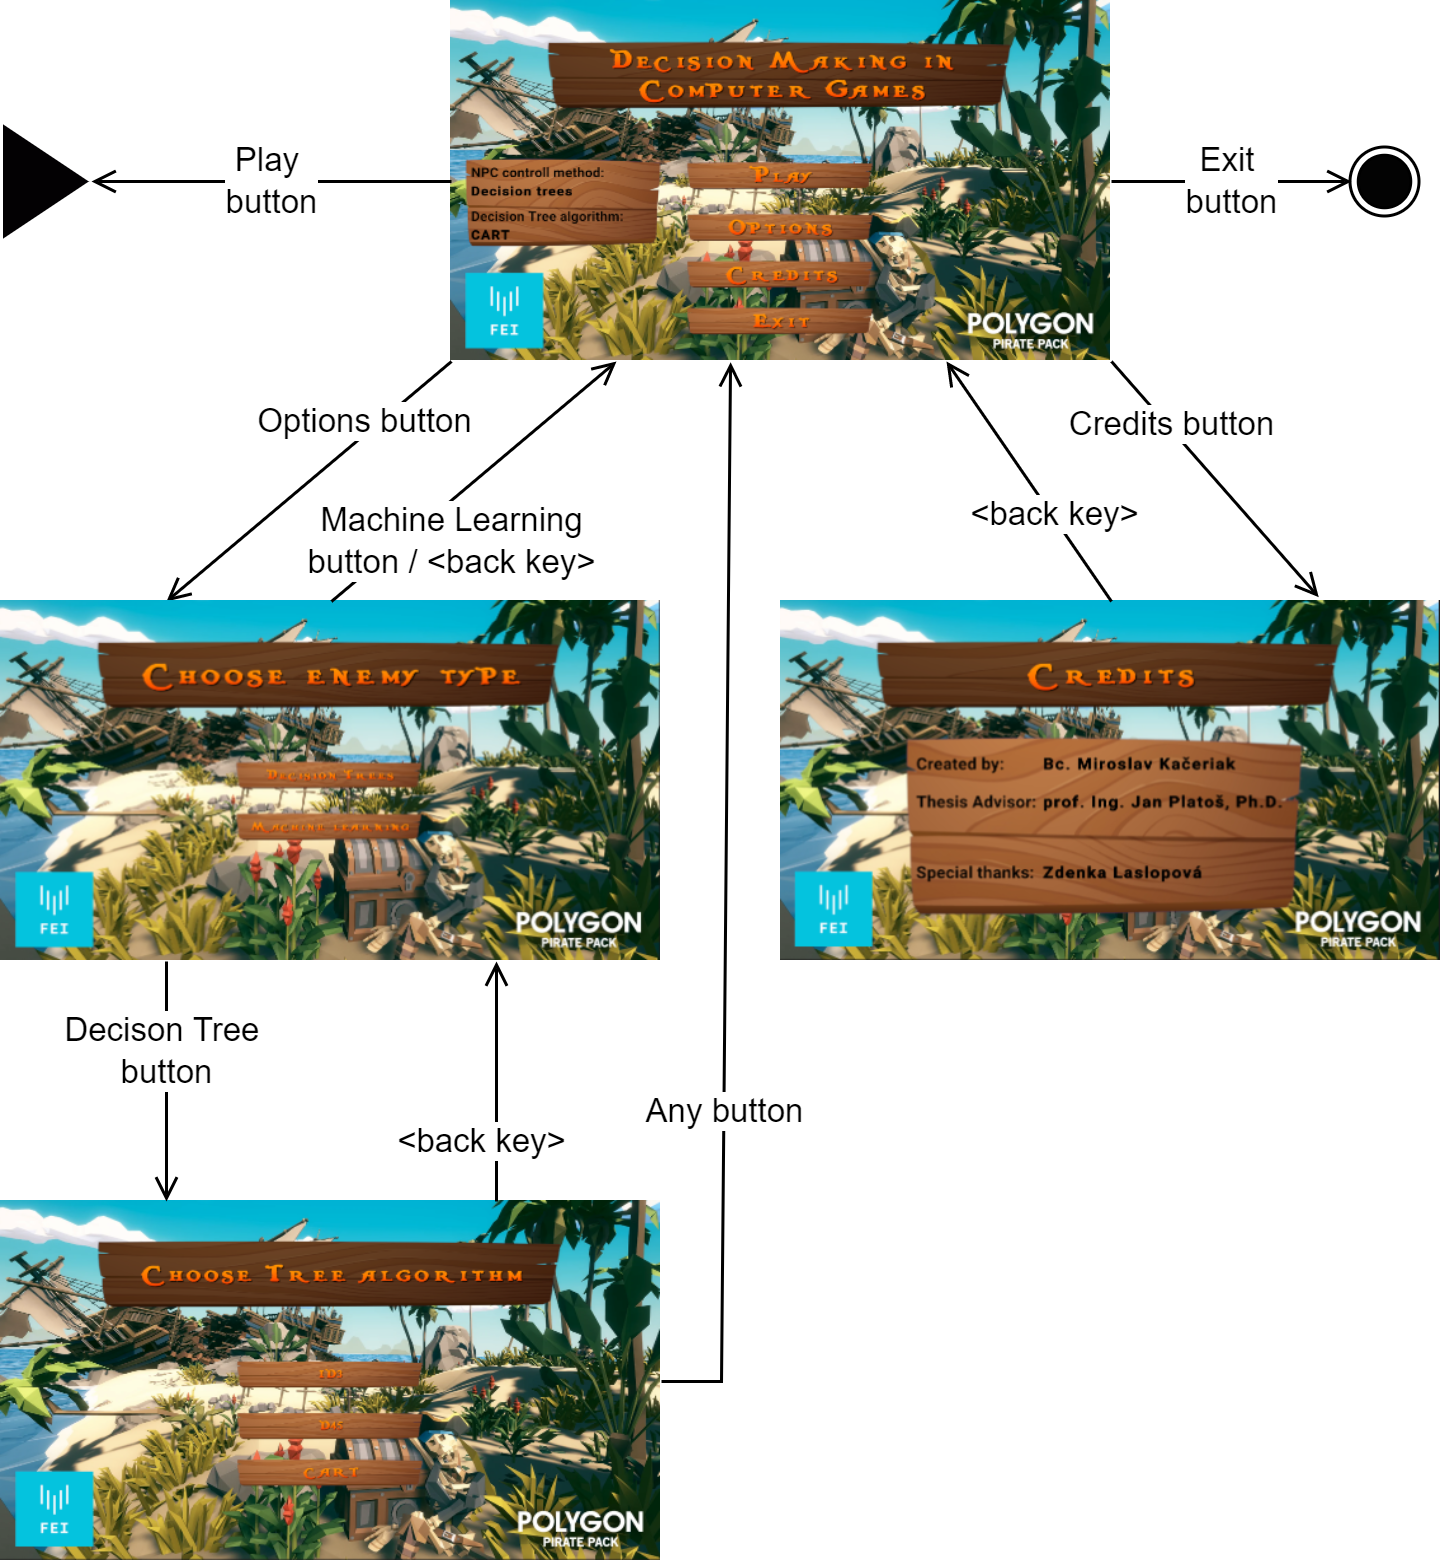
\includegraphics[width=.85\textwidth]{Figures/mainMenuScheme.png}
	\caption{Diagram obrazoviek hlavnej ponuky}
	\label{pic:MainMenuScheme}
\end{figure}

% Chapter 5
\chapter{Architektúra hráčskej postavy}
\label{sec:Player}
Jednou z najdôležitejších súčasti hier ovládaných z pohľadu tretej osoby je práve hráčska postava. Tá reaguje na hráčov vstup zmenou smeru alebo rýchlosti pohybu, akciami ako napríklad skok, útok, úhyb či kontextuálnou interakciou s nejakým objektom v hre a podobne. Na postavu hráča zvykne taktiež pôsobiť určitá forma gravitácie a s tým súvisiaca kolízia s hernou plochou a ostatnými statickými či dynamickými objektami. Hráčska postava má spravidla nastavenú nejakú hodnotu zdravia (života), ktorá sa v čase mení napríklad po páde z veľkej výšky či po zásahu od nepriateľa. Hodnota ostávajúceho zdravia je často hráčovi prezentovaná vo forme GUI ukazovateľa. 

Táto kapitola popisuje akým spôsobom bolo k jednotlivým problémom pristupované v tomto projekte. Niektoré princípy je možné s väčšími či menšími úpravami aplikovať obecne, iné sú poplatné enginu Unity. 

\section{Prehľad komponentov}
\label{sec:PlayerComponentOverview} 
Samotný objekt hráčskej postavy sa skladá z dvoch objektov, ktoré sa zvyknú nazývať kontroler a model. 

Model reprezentuje vizuálnu stránku objektu, teda postavu samotnú a ďalšie menšie objekty, ktoré táto postava nosí na sebe. Pri zložitejších modeloch môže ísť o hierarchiu čítajúcu stovky objektov, ktoré reprezentujú jednotlivé časti tela či ďalšie objekty. V tomto prípade je využitý tzv. low poly model, ktorý je vcelku a pod sebou má iba zopár vizuálnych doplnkov, ktoré postava nosí okolo pása. Low poly modely hráčskej postavy, nepriateľov a prostredia pochádzajú z balíka POLYGON Pirates \cite{Synty} od spoločnosti Synty Studios zakúpeného v oficiálnom online obchode enginu Unity.

Kontroler, na druhú stranu obsahuje sadu komponentov, ktoré obstarávajú pohyb, gravitáciu, kolíziu a ľubovoľnú ďalšiu funkcionalitu. Dôležitou súčasťou kontrolera je práve Unity komponenta Character Controller. Na nej je možné nastaviť rôzne parametre definujúce tvar kolíznej kapsule, maximálnu výšku kroku, ktorý môže postava vykonať bez nutnosti vyskočiť apod. Túto kapsulu s kompletnou vizuálnou stránkou hráča je možné vidieť na obrázku \ref{pic:PlayerController}.

\begin{figure}[!htbp]
	\centering
	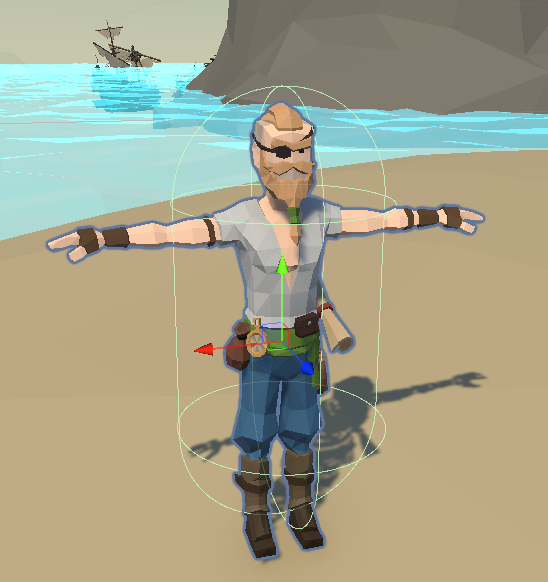
\includegraphics[width=0.54\textwidth]{Figures/controller.png}
	\caption{Hráčka postava s komponentou Character Controller}
	\label{pic:PlayerController}
\end{figure}

Na objekte kontroler sa ďalej nachádzajú komponenty PlayerBrain, PlayerBody, PlayerMovement, PlayerAutomaticMovement a NavMeshAgent. Posledné dve spomenuté komponenty sú v predvolenom stave deaktivované a aktivuje ich komponenta PlayerBrain v prípade, že má objekt ConfigManager v editore nastavenú premennú PlayerControll na hodnotu Automatic. Toto je využívané primárne v trénovacích scenároch, ktoré sú bližšie popísané v kapitole \ref{sec:Training}. V tomto prípade taktiež komponenta PlayerBrain deaktivuje komponentu PlayerMovement, čím znemožní ovládať hráča pomocou vstupu z periférií. 

Poslednou kompetenciou komponenty PlayerBrain je uchovávať referencie na zvyšné komponenty a inicializovať ich. Počas inicializačnej fázy sú jednotlivým komponentám predané referencie na iné komponenty ktoré potrebujú pre svoje fungovanie. Tento prístup umožňuje centrálne riadiť prepojenia medzi komponentami bez nutnosti ich rôzne referencovať navzájom v editore.

\section{Prijímanie poškodenia}
\label{sec:DealingDamage}
Hráčska postava je zraniteľná voči útoku nepriateľského NPC agenta. Maximálna hodnota poškodenia, ktorú hráčska postava môže inkasovať kým zomrie je nastavená v komponente PlayerBody. Táto komponenta teda obsahuje maximálnu hodnotu zdravia, ktorá sa hráčovi nastaví na začiatku hry a aktuálnu hodnotu zdravia, ktorá klesá s prijímaným poškodením. Všetká potrebná funkcionalita súvisiaca s prijímaním poškodenia vrátane propagovania informácie o zmene hodnoty zdravia či smrti danej postavy bola zjednotená pod rozhranie IDamageable. Toto rozhranie okrem komponenty PlayerBody implementuje aj abstraktná komponenta NPCBody, ktorá bude bližšie popísaná v kapitole \ref{sec:Agents}. Spomínané rozhranie je možné vidieť vo výpise \ref{src:IDamageable}. 

\vspace{8pt}
\begin{lstlisting}[label=src:IDamageable,caption={Rohranie IDamageable}]
public interface IDamageable
{
    public float MaxHealth { get; }
    public float Health { get; }

    public event Action<float> OnHealthChanged;
    public event Action OnDied;

    public void DealDamage(float damage);
}
\end{lstlisting}

Komponenta PlayerBody sa pri spustení hry zaregistruje pod objekt GameManager ako implementácia rozhrania IDamageable. GameManager sa v tomto momente stane odberateľom eventu OnHealthChanged za účelom aktualizácie GUI elementu zobrazujúceho aktuálny stav zdravia hráčskej postavy. Tento element sa zvykne nazývať Health bar.

Zavolanie metódy DealDamage() na hráčskej postave teda spôsobí odrátanie hodnoty poškodenia od aktuálnej hodnoty zdravia a vyvolanie spomínaného eventu. Pokiaľ táto hodnota zdravia klesne na nulu je na hráčskej postave deaktivované ovládanie pohybu a vyvolá sa event OnDied. Na tento event zareaguje odberateľ GameManager, ktorý vyvolá event OnGameEnded, na základe ktorého sa deaktivuje ovládanie kamery a následne je hráčovi zobrazená informácia o konci hry. Po určitom čase je scéna reštartovaná a hráč to môže skúsiť znova a lepšie. 

Informáciu o konci hry spolu s prázdnym GUI elementom Health bar je možné vidieť na obrázku \ref{pic:YouDied}. Na tomto obrázku je možné povšimnúť si aj GUI elementy zobrazujúce hráčovi počet nazbieraných predmetov spolu s minimálnym počtom, ktorý je vyžadovaný na úspešné dokončenie hry. 
%Aktualizácia počtu zozbieraných predmetov v GUI je záležitosťou nastavenia reťazca v premennej text príslušného objektu. 

GUI element Health bar sa skladá z troch častí: výplň, obrys a ikona srdca. Na aktualizáciu hodnoty v tomto GUI elemente je využívaná Unity komponenta Slider. Táto komponenta má množstvo nastavení a parametrov vrátane objektu, ktorého rozmery bude Slider ovplyvňovať (v tomto prípade výplň elementu) a maximálnej hodnoty. Tá sa pri spustení hry nastaví na hodnotu maximálneho zdravia hráčskej postavy a je teda možné priamo bez prepočtu nastavovať hodnotu Slideru v reakcii na zmenu zdravia hráča.

\begin{figure}[!htbp]
	\centering
	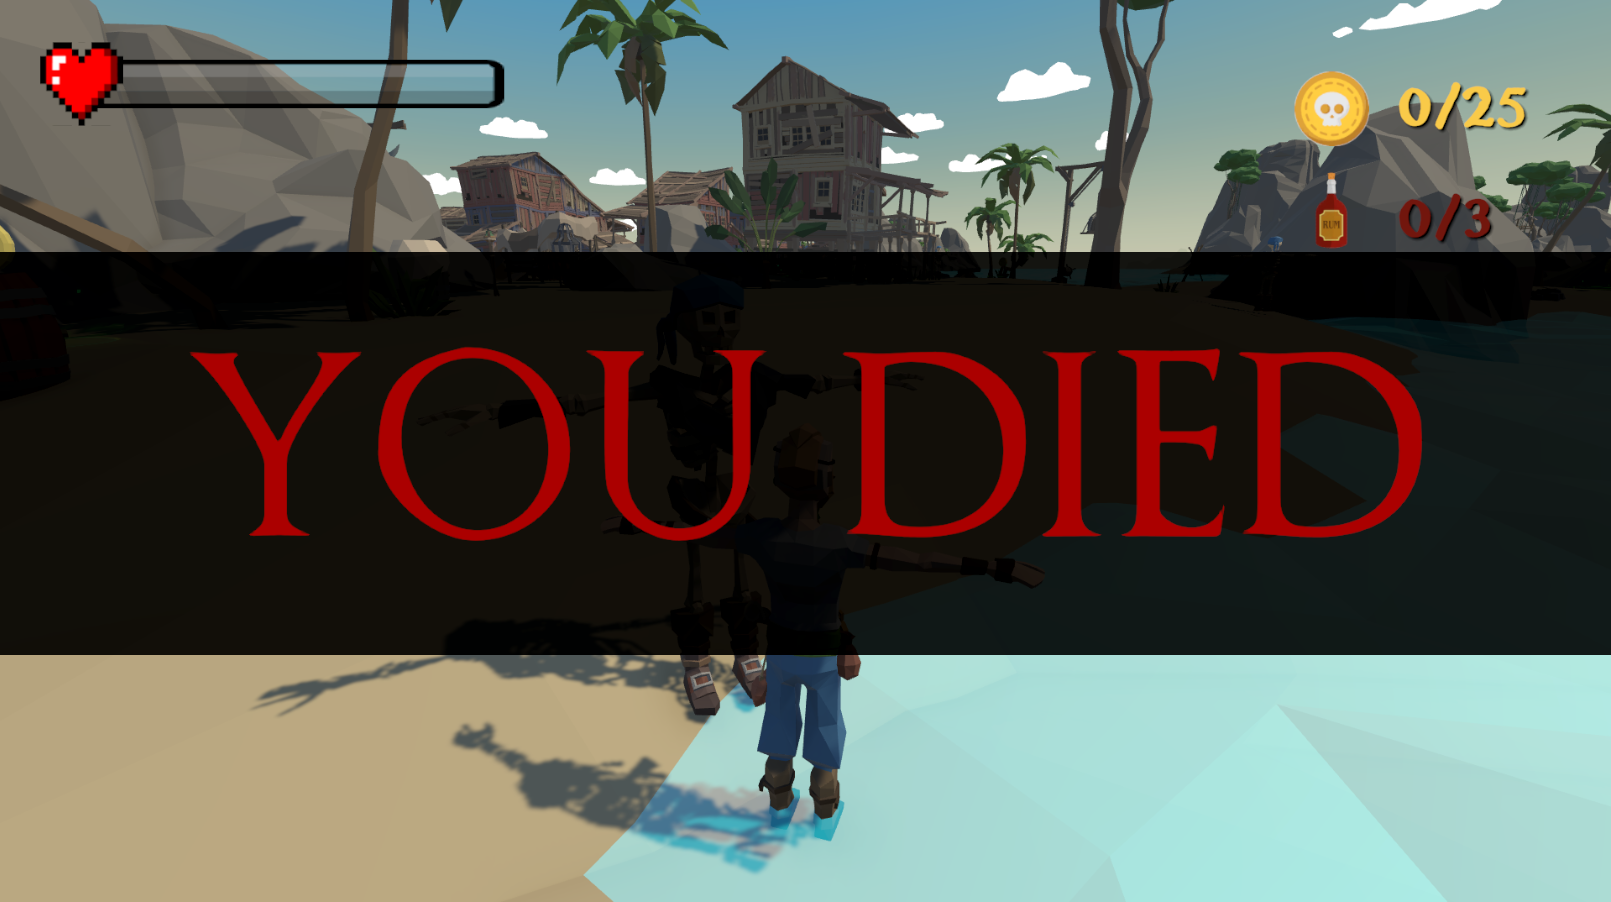
\includegraphics[width=.8\textwidth]{Figures/youDied.png}
	\caption{GUI elementy v hlavnej scéne}
	\label{pic:YouDied}
\end{figure}

\section{Pohyb}
\label{sec:PlayerMovement} 
Jednou z najdôležitejších súčastí hráčskej postavy je práve možnosť jej ovládania pomocou periférií. Pre tento účel bola vytvorená komponenta PlayerMovement. Tá periodicky obstaráva komunikáciu s objektom InputManager, z ktorého získané vstupy transformuje na pohyb postavy v trojrozmernom hernom priestore pomocou komponenty Character Controller.

Existuje množstvo prístupov k tejto problematike a v závislosti od typu hry či členitosti herného prostredia môže byť práve pohyb hráča veľmi komplexnou témou hlavne v kombinácií s realistickými animáciami.

V tomto projekte bol využitý základný systém využívajúci možností vstavanej Unity komponenty Character Controller a to ako na pohyb tak aj na zisťovanie, či sa hráč nachádza na pevnej zemi. Hráčovi je okrem základného pohybu do rôznych smerov umožnené skákať, či spomaliť svoj pohyb, čím sa zníži rozsah šírenia zvuku jeho krokov. Pohyb hráča taktiež podlieha základnej simulácií gravitácie. Metódu Update() komponenty PlayerMovement, ktorá obstaráva vyššie popísanú funkcionalitu je možné vidieť vo výpise \ref{src:PlayerMovement}.

\vspace{8pt}
\begin{lstlisting}[label=src:PlayerMovement,caption={Realizácia pohybu hráčskej postavy}]
void Update()
{
    var currentSpeed = speed;

    if (controller.isGrounded)
        UpdateGrounded(ref currentSpeed);

    Vector3 direction = new Vector3(horizontal, 0, vertical);
    float magnitude = Mathf.Clamp01(direction.magnitude) * currentSpeed;
    direction.Normalize();

    float angle = SmoothAngleFromDirection(direction);
    if (direction != Vector3.zero)
        transform.localRotation = Quaternion.Euler(0f, angle, 0f);

    Vector3 moveDirection = Quaternion.Euler(0f, angle, 0f) * Vector3.forward;
    Vector3 velocity = moveDirection.normalized * magnitude;

    ySpeed += Physics.gravity.y * Time.deltaTime;
    velocity.y = ySpeed;

    controller.Move(velocity * Time.deltaTime);
    MakeNoise(velocity);
}
private void UpdateGrounded(ref float currentSpeed)
{
    ySpeed = defaultYSpeed;

    horizontal = inputManager.Horizontal;
    vertical = inputManager.Vertical;

    if (inputManager.WasJumpingThisFrame)
        ySpeed = jumpSpeed;

    if (inputManager.IsCrounching)
        currentSpeed /= 2;
}
\end{lstlisting}

Vo výpise \ref{src:PlayerMovement} je možné si povšimnúť, že pokiaľ sa hráčska postava nachádza na zemi, je možné zmeniť jej smer na osách X a Z, vyskočiť, či znížiť rýchlosť pohybu na polovicu, čo sa prejaví pri šírení zvuku krokov. V tomto prípade je aj vyresetovaná rýchlosť postavy na ose Y a to na hodnotu 0. V momente kedy hráč stlačí tlačidlo skoku, je táto rýchlosť nastavená na hodnotu výšky skoku a počas nasledujúcich snímkov bude klesať rýchlosťou gravitačnej konštanty vynásobenej časom medzi jednotlivými snímkami. Keď postava dopadne na zem, je táto rýchlosť opäť vyresetovaná a medzi jednotlivými snímkami sa mení len minimálne v závislosti od hodnoty FPS a teda mierne tlačí postavu k zemi, čím sa eliminujú problémy s prípadnou zlou detekciu zeme pri nerovnom teréne.

Následne sa na základe hráčskeho vstupu vypočíta smer a rýchlosť pohybu, ktorým sa má postava vydať a výsledná hodnota, opäť vynásobená časom medzi jednotlivými snímkami, je odoslaná do metódy Move() komponenty Character Controller. Táto metóda vykoná pohyb postavy, pokiaľ to kolízna kapsula či výška nerovného terénu dovolí. Násobenie hodnotou Time.deltaTime, teda časom medzi jednotlivými snímkami spôsobí, že rýchlosť pohybu bude nezávislá od snímkovej frekvencie hry.

Taktiež je vhodné neaplikovať smer na rotáciu postavy priamo, ale vziať do úvahy aktuálnu rotáciu kamery, teda smer, do ktorého sa hráč pozerá. Z dôvodu eliminácie instantnej zmeny rotácie, čo spôsobí nepríjemný efekt teleportácie modelu do daného smeru je tiež vhodné robiť veľké zmeny postupne. Tento prístup je znázornený vo výpise \ref{src:SmoothAngleFromDirection}.

\vspace{8pt}
\begin{lstlisting}[label=src:SmoothAngleFromDirection,caption={Postupná zmena rotácie postavy v súlade s rotáciu kamery}]
private float SmoothAngleFromDirection(Vector3 direction)
{
    var cameraY = (cameraTransform == null) ? 
    cameraTransform.eulerAngles.y : 0.0f;

    float tempAngle = Mathf.Atan2(direction.x, direction.z) * Mathf.Rad2Deg + cameraY;
    return Mathf.SmoothDampAngle(transform.eulerAngles.y, tempAngle, ref turnSmoothVelocity, turnSmoothTime);
}
\end{lstlisting}

Poslednou kompetenciou komponenty PlayerMovement je vydávanie zvuku pri pohybe. To je realizované pomocou metódy MakeNoise() vo výpise \ref{src:PlayerMovement}. Táto metóda na základe vstupného parametru, ktorý reprezentuje rýchlosť pohybu vypočíta druhú mocninu dĺžky X a Z zložky vstupného vektoru. Tú spolu s aktuálnou pozíciou vloží ako parametre koštruktoru readonly štruktúry Noise a následne zavolá na objekte SoundManager metódu MakeNoise, ktorej danú inštanciu štruktúry odošle ako parameter. Tento postup sa vykonáva v pravidelných intervaloch, ktorých dĺžka je daná konštantou stepDelay a za splnenia podmienky, že hráč nie je statický. 

SoundManager následne vytvorí tzv. SphereCast a teda získa všetky kolidery v rádiuse daného bodu v priestore. Všetky nájdené objekty sú skontrolované na prítomnosť komponenty Hearing. Ak objekt obsahuje túto komponentu, je na nej zavolaná metóda RespondToNoise(), ktorej je predaná pozícia danej inštancie zvuku. Reakcia na tento podnet je bližšie popísaná v kapitole \ref{sec:Agents}. Pomocou Unity metódy OnDrawGizmosSelected() bola taktiež v editore vytvorená jednoduchá vizualizácia zvuku za účelom ladenia

\section{Kamera}
\label{sec:Camera}
Kamera je veľmi dôležitým prvkom každej hry. Nielenže hráč pomocou nej môže sledovať dianie v hernom svete, ale už samotným pohybom tejto kamery môže ovplyvňovať napríklad smer pohybu hráčskej postavy, čo bolo demonštrované v predchádzajúcej sekcií. 

V editore Unity je možné využiť na snímanie diania v hre predpripravenú komponentu Camera. Tá umožňuje nastavenie rôznych parametrov ako FOV, typ projekcie, vzdialenosť orezávacích rovín, anti-aliasing apod. Bez prítomnosti kamery v scéne je renderovaná iba čierna obrazovka s varovným nápisom a GUI. Kamier v scéne môže byť niekoľko a je možné medzi nimi plynulo prepínať napríklad v rámci filmových sekvencií čí mierenia so zbraňou.

Ovládanie kamery bolo realizované pomocou rozšírenia Cinemachine od spoločnosti Unity, ktorá vytvára aj samotný engine. Toto rozšírenie je zdarma dostupné z oficiálneho repozitára a obsahuje niekoľko typov kamier, ktoré je možné použiť. V tomto projekte je využitá tzv. Free Look Camera. Po výbere kamery je na objekt, ktorý obsahuje Unity komponentu Camera pridaná komponenta CinemachineBrain a následne je vytvorený nový herný objekt, ktorý reprezentuje vybraný typ kamery. CinemachineBrain sa s týmto novým objektom prepojí a ten prevezme kontrolu nad pozíciou a rotáciou pôvodnej kamery bez nutnosti ručného nastavovania týchto parametrov zo skriptu.

\begin{figure}[!htbp]
    \centering
    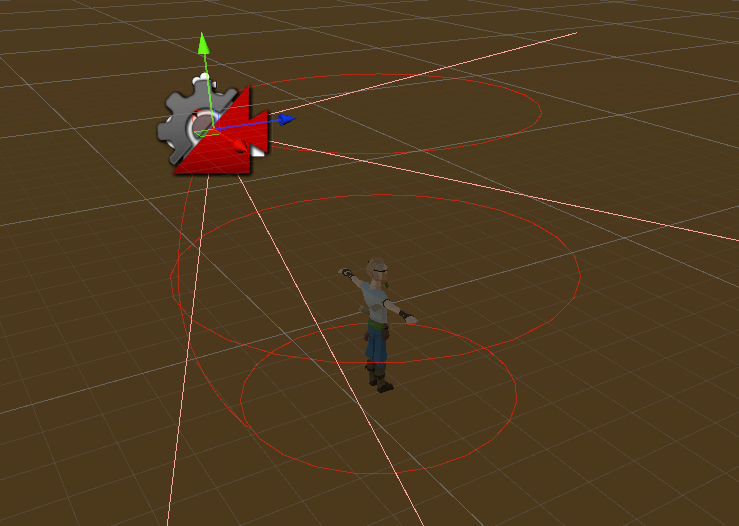
\includegraphics[width=.85\textwidth]{Figures/obruce.png}
    \caption{Vizualizácia obručí, po ktorých sa pohybuje herná kamera}
    \label{pic:Cinemachine}
\end{figure}

Komponenta ovládajúca kameru má veľké množstvo nastavení, ktorých popis by presahoval rámec tejto práce. Dôležitým parametrami sú hlavne referencie na objekt, ktorý má kamera prenasledovať a na ktorý sa má zamerať. V tomto prípade bola na oba prípady využitá referencia hráčskej postavy. Ďalej boli na tomto mieste nastavené rýchlosti či rozsah pohybu kamery na jednotlivých osách, ktoré boli zároveň namapované na príslušné osy vstupných periférií. Kvôli kolízií kamery s hernými objektami bola ešte pridaná a nastavená komponenta Cinemachine Collider.

Samotná kamera sa potom pohybuje po troch obručiach - spodnej, strednej a hornej. Výšku a priemer týchto obručí je taktiež možné upraviť a každá z nich má separátne nastavenia, ktoré určujú stred pohľadu kamery, mŕtvu zónu, rýchlosť s akou sa kamera snaží dohnať svoj cieľ apod. Tieto obruče sú pre lepšiu predstavu znázornené na obrázku \ref{pic:Cinemachine}.

%Chapter 6
\chapter{Architektúra NPC agentov}
\label{sec:Agents}
Ako už bolo spomenuté v predchádzajúcich kapitolách, projekt obsahuje dva typy NPC agentov. Prvý typ sa rozhoduje na základe rozhodovacieho stromu zostrojeného zo vstupných dát a druhý typ agentov využíva na rozhodovanie model natrénovaný pomocou reinforcement learningu. Jednotlivé typy NPC sa líšia aj v prístupe k navigácií priestorom či kolízií a ďalšími detailami v skladbe či funkcionalite jednotlivých komponentov. Táto kapitola si kladie za cieľ popísať štruktúru jednotlivých typov NPC, ich spoločné vlastnosti a odlišnosti s dôrazom na percepciu, teda zmyslové vnímanie jednotlivých NPC agentov.

\section{Spoločné prvky oboch typov agentov}
\label{sec:AgentsBoth}

Prvým spoločným prvkom NPC agentov je ich inštancovanie. Túto funkcionalitu obstaráva objekt EnemySpawner nachádzajúci sa v scéne. Potomkami tohto objektu v hierarchií sú prázdne objekty, tzv. spawn pointy, ktoré boli ručne rozmiestnené po hernej ploche. V momente spustenia scény sú z nich získané tzv. Transform komponenty, ktoré združujú pozíciu, rotáciu a mierku objektu. Tie potom pri procese inštancovania zabezpečujú, že objekt bude inštancovaný na určenú pozíciu v hernom svete a s určenou rotáciou. Pri tomto procese je ešte nutná referencia na tzv. prefab herného objektu a voliteľným prvkom je objekt, ktorý sa stane rodičom novo inštancovaných objektov. 

Prefab v editore Unity je možné chápať ako šablónu herného objektu spolu s jeho komponentami, nastavenými hodnotami a podradenými hernými objektami. Túto šablónu je možné opakovane použiť v rámci jednej alebo viacerých scén. Tento systém ponúka efektívny spôsob správy herných objektov a synchronizáciu zmien bez nutnosti opakovaných úprav každej kópie. Túto synchronizáciu je možné vyvolať aj ručne, čo umožňuje robiť zmeny len na konkrétnych kópiách a nepropagovať ich ďalej, či priamo vytvárať prefab ako variantu už existujúceho. Taktiež umožňujú jednoduché inštancovanie herných objektov za behu, bez nutnosti opakovane im nastavovať rovnaké hodnoty či priraďovať určité komponenty alebo podradené herné objekty po inštancovaní. Jednotlivé prefaby je možné aj hierarchicky zanorovať do seba \cite{Prefabs}.

Proces inštancovania NPC agentov, ktorý je možné vidieť vo výpise \ref{src:GameManOnStart}, vyvoláva už spomínaný objekt GameManager na základe nastavení uložených v objekte ConfigManager. Volaná metóda určuje, ktorý konkrétny prefab bude pri inštancovaní použitý.

\vspace{8pt}
\begin{lstlisting}[label=src:GameManOnStart,caption={Inštancovanie NPC agentov v závislosti od nastavení}]
public void OnStart() 
{
    if (!spawner)
        return;

    var controllMethod = MainManager.Instance.ConfigManager.NPCControll;

    if (controllMethod == ENPCControllMethod.DecisionTrees)
        spawner.SpawnRegularEnemies();
    else if (controllMethod == ENPCControllMethod.ReinforcementLearning)
        spawner.SpawnMLEnemies();
    else
        throw new Exception("Invalid NPC controll method");
}
\end{lstlisting}

Vo výpise \ref{src:GameManOnStart} je možné si povšimnúť, že pre využitie možností životného cyklu objektu nie je využitá metóda Start() ale vlastná metóda OnStart(), ktorá je volaná z metódy Start() objektu MainManager. Tento prístup má dve hlavné výhody. Prvou je dosiahnutie lepšieho výkonu, nakoľko stačí z natívneho C++ kódu volať určitú metódu životného cyklu iba na jednom hlavnom objekte a ten sa postará o volanie vo zvyšných objektoch, ktoré spravuje. Ďalšou výhodou, ktorá bola v tomto prípade dôležitejšou, je možnosť riadiť poradie, v akom budú metódy volané na konkrétnych objektoch a nenechávať to na rozhodnutí herného enginu. Ak by sa v tomto prípade objekt GameManager inicializoval skôr ako ConfigManager boli by použité prednastavené hodnoty a nie dáta deserializované z perzistentného úložiska nastavení. 

Ďalším spoločným prvkom oboch typov NPC je komponenta Capsule Collider. Ide o podobnú kapsulu akú obsahuje Character Controller ale jej jedinou úlohou je obstarávať kolíziu s prostredím narozdiel od Character Controlleru, ktorý obsahuje aj ďalšiu funkcionalitu. Taktiež je možné nastaviť stred, výšku, čí polomer kapsule. Podobne ako komponentu Box Collider na objekte Finish je možné ju nastaviť ako trigger, kedy vyvoláva príslušný event pri strete s iným objektom, ale je ignorovaná fyzikálnym enginom a teda negeneruje kolíziu v pravom slova zmysle.

Oba typy NPC zdieľajú komponentu SkeletonBody, ktorá je konkretizáciou triedy NPCBody. Tá určuje konkrétne hodnoty parametrov ako rýchlosť, dosah či maximálnu hodnotu zdravia, ktoré môžu byť prispôsobené na mieru konkrétnemu NPC či archetypu. Rovnako ako komponenta \mbox{PlayerBody} spomínaná v sekcií \ref{sec:DealingDamage} implementuje NPCBody rozhranie IDamageable, uvedené vo výpise \ref{src:IDamageable}, so všetkým, čo to obnáša. Okrem toho však poskytuje informácie o stave NPC samotného ako aj jeho zmyslov, čo je následne použité pri rozhodovacom procese.

Posledným spoločným prvkom je komponenta Hearing, ktorá obstaráva počutie NPC agentov. Táto komponenta implementuje generické rozhranie ISense<T>, ktoré reprezentuje každý zo zmyslov agenta. V tomto prípade je ako generikum použitá spomínaná štruktúra Noise. Rozhranie samotné je možné vidieť vo výpise \ref{src:ISense}.

\vspace{8pt}
\begin{lstlisting}[label=src:ISense,caption={Generické rozhranie ISense}]
public interface ISense<T>
{
    bool IsActivated { get; }
    float DistanceToTarget { get; }
    T Target { get; }

    bool TryGetTarget(out T outTarget);
}
\end{lstlisting}

Nad rámec funkcionality rozhrania ponúka komponenta Hearing verejnú metódu RespondToNoise(), ktorá je na danom agentovi zavolaná v momente, keď ho zasiahne SphereCast vyvolaný objektom SoundManager. V tejto metóde sú následné nastavené všetky verejné vlastnosti triedy poskytované rozhraním. Vzdialenosť k cieľu je potom periodicky aktualizovaná až do momentu, kedy agent prekročí nastavenú prahovú vzdialenosť, čo spôsobí nastavenie verejných vlastnosti do pôvodných hodnôt. Hodnoty týchto vlastností sú potom využívané pri rozhodovacom procese popísanom v nasledujúcich sekciách.

\section{NPC agenti ovládaní rozhodovacím stromom}
\label{sec:AgentsWithTrees}
Jednou z vecí, ktorá musela byť pre každý typ NPC agentov realizovaná odlišne, je pohyb. U agentov ovládaných rozhodovacím stromom tento aspekt realizuje tzv. Navmesh. Práca s Navmeshom zahŕňa dve hlavné komponenty: NavMeshSurface a NavMeshAgent. 

NavMeshSurface slúži na definovanie oblasti, po ktorej sa objekt obsahujúci komponentu NavMeshAgent môže pohybovať. Táto oblasť sa potom nazýva NavMesh a je nutné ju tzv. zapiecť nanovo pri každej manipulácií so statickými objektami v scéne. NavMeshSurface obsahuje množstvo nastavení ako napríklad typ agenta a geometrie, podľa ktorých vygeneruje NavMesh. Typ geometrie určuje, či sa má na generovanie NavMeshu využiť reálny objekt alebo jeho zjednodušená fyzikálna reprezentácia. Typ agenta potom ovplyvňuje parametre ako šírka či výška, na základe ktorých sa NavMesh nevygeneruje v miestach, na ktoré je agent moc vysoký a ani bezprostredne pri objektoch, do ktorých by mohli zasahovať časti jeho tela \cite{NavMeshSurface}. Komponentu NavMeshSurface je možné umiestniť na ľubovoľný objekt, v tomto prípade bol však v scéne vytvorený separátny objekt obsahujúci iba túto komponentu. 

Finálny Navmesh vygenerovaný pre časť hernej oblasti je možné vidieť na obrázku \ref{pic:NavMesh}. Môžeme si povšimnúť, že bol vygenerovaný aj na strechách budov, ktorých stúpanie odpovedá maximálnej nastavenej výške kroku. Toto chovanie je možné potlačiť na konkrétnych objektoch ručne, avšak medzi jednotlivými segmentami neboli vygenerované linky po ktorých by agent mohol vyskočiť a teda sa na tieto miesta nedostane, pokiaľ tam nie je explicitne umiestnený spawn point. 

\begin{figure}[!htbp]
    \centering
    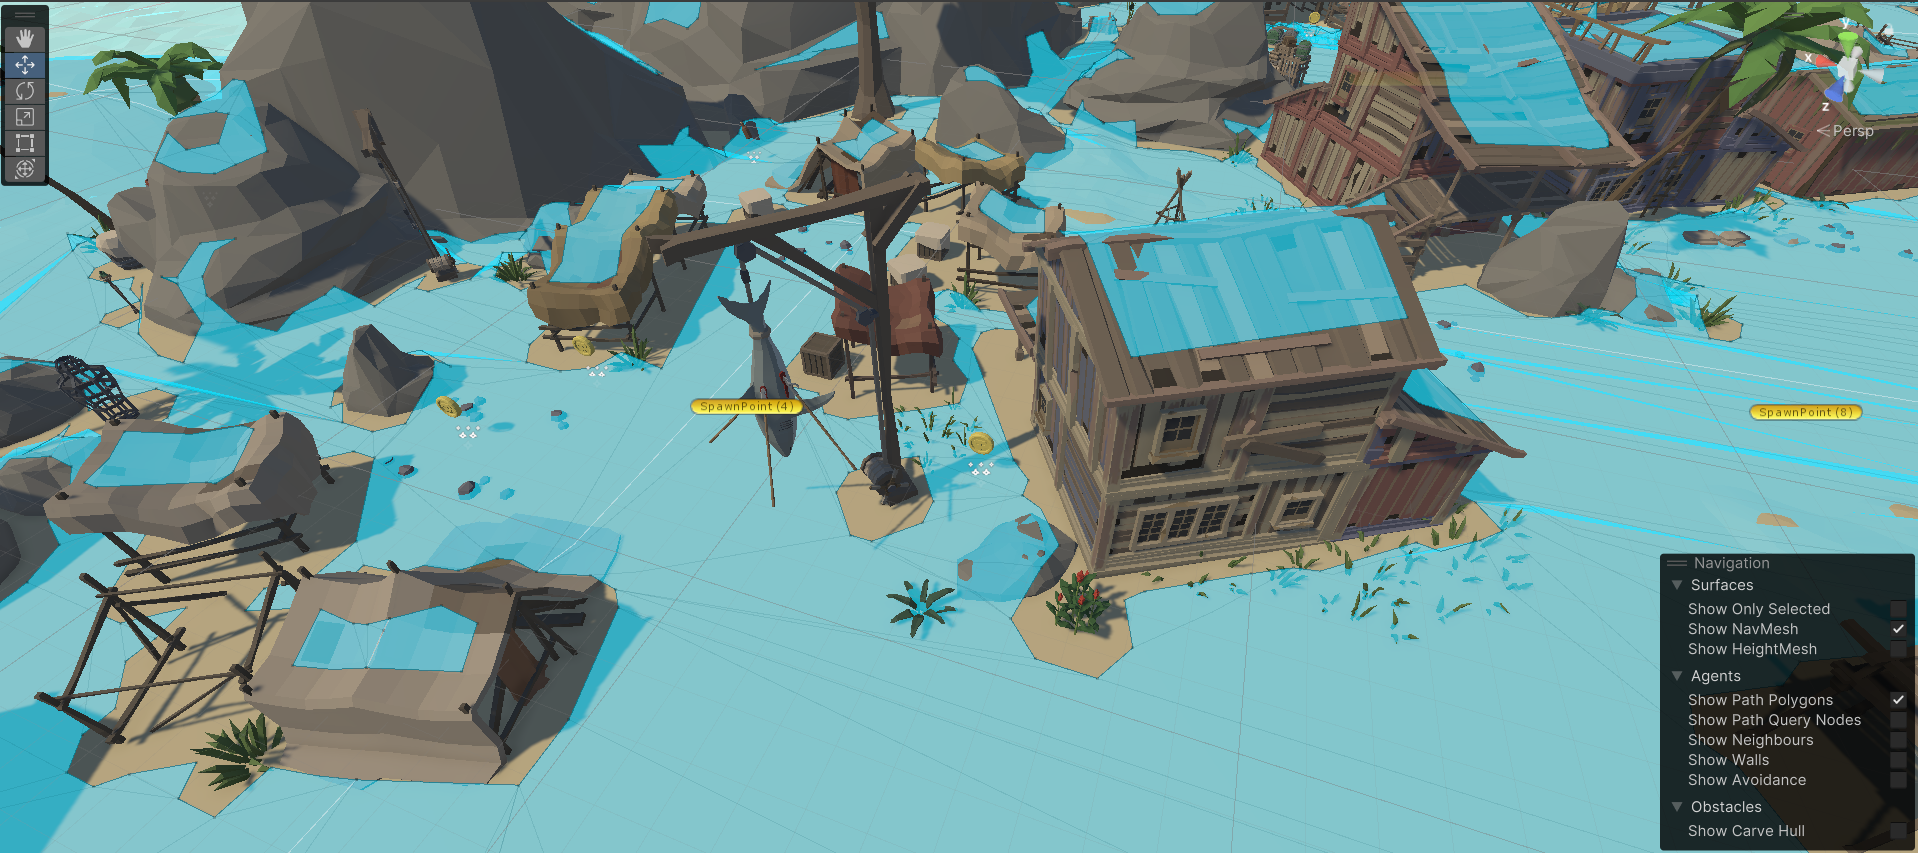
\includegraphics[width=1\textwidth]{Figures/navmesh.png}
    \caption{Vygenerovaný NavMesh pre hernú oblasť}
    \label{pic:NavMesh}
\end{figure}

Komponenta NavMeshAgent sa, ako názov napovedá, pridáva priamo na NPC agenta, kde je okrem spomínaného typu možné nastaviť aj rýchlosť, akceleráciu, či tzv. stoppingDistance, ktorá definuje, ako ďaleko pred cieľovým bodom sa agent má zastaviť. Okrem toho je možné na tejto komponente upraviť aj rôzne parametre týkajúce sa vyhýbaniu prekážkam. Cieľ je možné agentovi nastaviť priamo z kódu zavolaním metódy SetDestination(), ktorá sa pokúsi po vygenerovanom NavMeshi nájsť najkratšiu cestu k cieľovému bodu, ak takáto cesta existuje.

Ďalším špecifikom agentov ovládaných rozhodovacím stromom je komponenta EyeSight reprezentujúca videnie agenta. Schopnosť videnia má samozrejme aj druhý typ agenta, tá je však z dôvodov popisovaných v nasledujúcej kapitole realizovaná odlišne.

Komponenta EyeSight, podobne ako komponenta Hearing, implementuje generické rozhranie ISense<T> \ref{src:ISense}, tentokrát je však generikom samotný herný objekt. Nad rámec implementácie rozhrania je na tejto komponente možné nastaviť masku vrstvy hráča na ktorú reaguje príslušný RayCast a masku vrstvy prekážok, cez ktorú RayCast naopak neprejde. Taktiež je tu možné nastaviť parametre definujúce FOV ako polomer kružnice okolo agenta či uhol v rozsahu 0$^{\circ}$--360$^{\circ}$.

Na rozdiel od komponenty Hearing, ktorá reaktívne odpovedá na podnety prostredia, komponenta EyeSight aktívne kontroluje prítomnosť hráčskej postavy v zornom poli. Na tento účel je vytvorená korutina EyeSightCoroutine(), ktorá je spustená v metóde Start() príslušného agenta. Túto korutinu je možné vidieť vo výpise \ref{src:EyeSightCoroutine}.

\vspace{8pt}
\begin{lstlisting}[label=src:EyeSightCoroutine,caption={Korutina zabezpečujúca videnie agenta}]
private IEnumerator EyeSightCoroutine()
{
    float delay = 0.2f;
    var wait = new WaitForSeconds(delay);

    while (isActive)
    {
        yield return wait;
        CheckEyeSight();
    }
}
private void CheckEyeSight()
{
    this.target = null;
    isActivated = false;
    this.distanceToTarget = float.MaxValue;

    Collider[] rangeChecks = Physics.OverlapSphere(transform.position, radius, targetMask);
    if (rangeChecks.Length == 0)
        return;

    Transform target = rangeChecks[0].transform;
    Vector3 directionToTarget = (target.position - transform.position).normalized;

    if (Vector3.Angle(transform.forward, directionToTarget) > angle / 2)
        return;

    float targetDistance = Vector3.Distance(transform.position, target.position);
    if (Physics.Raycast(transform.position, directionToTarget, targetDistance, obstacleMask))
        return;

    isActivated = true;
    this.target = target.gameObject;
    this.distanceToTarget = targetDistance;
}
\end{lstlisting}

Korutina teda periodicky spúšťa v definovanom intervale metódu CheckEyeSight(). Tento prístup je výhodný z hľadiska výkonu, nakoľko pri testovaní sa ukázalo, že nie je nutné aktualizovať videnie agenta pri každom vykonaní hernej slučky. 

Metóda CheckEyeSight teda získa všetky kolidery v definovanom rádiuse. Nakoľko jediný objekt obsahujúci definovanú masku vrstvy je hráčska postava, je možné priamo vziať prvý prvok v poli koliderov, ak toto pole nie je prázdne a považovať ho za hráčsku postavu. Ak by agenti boli naprogramovaní na vzájomné reakcie medzi sebou, prípadne na špecifické objekty v scéne, stačilo by pridať masky týchto objektov do členskej premennej targetMask v editore, či pomocou binárnych operátorov v kóde a poľom preiterovať. Nakoľko sú ale kolidery získané v celom rozsahu kružnice, je následne získaný normalizovaný smer od agenta k cieľu a overené, čí vyhovuje nastavenému kruhovému výseku. Ak je táto podmienka splnená, vykoná sa RayCast, ktorý overí, či je medzi agentom a hráčom priama viditeľnosť. Ak je splnená aj táto podmienka, je možné do rozhodovacieho procesu zaviesť informáciu, o tom, že bol spozorovaný hráč.  

\begin{figure}[!htbp]
    \centering
    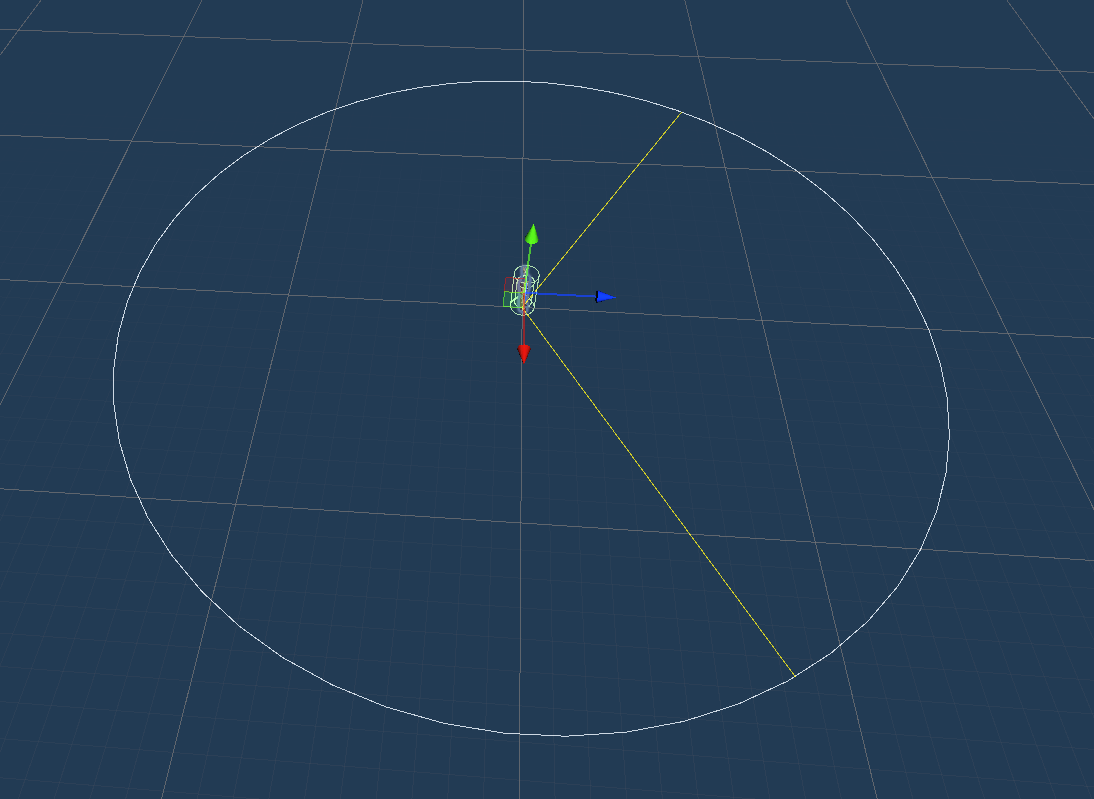
\includegraphics[width=.65\textwidth]{Figures/fov.png}
    \caption{Zorné pole NPC agenta ovládaného rozhodovacím stromom}
    \label{pic:FovDecision}
\end{figure}

Vizualizáciu zorného poľa NPC agenta využitú na ladenie je možné vidieť na obrázku \ref{pic:FovDecision}. Tá je realizovaná pomocou tzv. Custom Editoru pre triedu EyeSight, ktorý je vytvorený v Assembly-CSharp-Editor, teda osobitne od zvyšku tried, ktoré sú využívané v rámci buildu hry. V tomto editore je využitá metóda OnSceneGUI(), v ktorej je implementovaná logika vykreslovania kružnice a kruhového výseku v náhľade scény otvorenej v editore. Vizualizácia sa v reálnom čase aktualizuje v závislosti od nastavených parametrov v triede EyeSight.

\subsection{Rozhodovanie}
\label{sec:ImplDecisionTrees}
Rozhodovanie NPC ovládaných rozhodovacím stromom má na starosti abstraktná komponenta NPCBrain. Tá na začiatku svojho životného cyklu zavolá statickú metódu DecisionTree.FromFile(), ktorej parametrom je cesta k súboru. Obsah tohto súboru je následne využitý na zostrojenie výsledného rozhodovacieho stromu. Cesta ku konkrétnemu súboru je v tvare \textit{<Application.dataPath> /Data/<typ NPC>\_<algoritmus>.txt}. Typ NPC je určený overridnutím príslušnej premennej v potomkovi, algoritmus je potom daný nastavením v objekte ConfigManager. Metóda DecisionTree.FromFile() rekurzívne spracuje obsah súboru a vytvorí z neho inštanciu triedy DecisionTree, ktorá sa dá prechádzať jednotlivými NPC agentmi za behu aplikácie.

Dáta, z ktorých je vytváraný rozhodovací strom sú priamym výstupom algoritmov popísaných v sekcií \ref{sec:DecisionTreesOverview}. Pôvodný tvar dát využitých pri rozhodovaní NPC Skeleton je možné vidieť v tabuľke \ref{tab:skeletonActionRaw}.

\begin{table}[!ht]
    \centering
    \begin{tabular}{|c|c|c|c|c|}
    \hline
        \textbf{SeesEnemy} & \textbf{HearEnemy} & \textbf{EnemyInRange} & \textbf{HP} & \textbf{Action} \\ \hline
        FALSE & FALSE & FALSE & 100 & Idle \\ 
        FALSE & FALSE & TRUE & 50 & Idle \\ 
        FALSE & FALSE & FALSE & 25 & Idle \\ 
        FALSE & FALSE & TRUE & 65 & Idle \\ 
        TRUE & FALSE & TRUE & 40 & Attacking \\ 
        TRUE & TRUE & TRUE & 80 & Attacking \\ 
        TRUE & FALSE & TRUE & 10 & Attacking \\ 
        TRUE & TRUE & TRUE & 85 & Attacking \\ 
        FALSE & TRUE & TRUE & 60 & Seeking \\ 
        FALSE & TRUE & FALSE & 90 & Seeking \\ 
        FALSE & TRUE & TRUE & 15 & Seeking \\ 
        FALSE & TRUE & FALSE & 70 & Seeking \\ 
        TRUE & TRUE & FALSE & 20 & Chasing \\ 
        TRUE & FALSE & FALSE & 30 & Chasing \\ 
        TRUE & TRUE & FALSE & 35 & Chasing \\ 
        TRUE & FALSE & FALSE & 55 & Chasing \\ 
        TRUE & TRUE & TRUE & 0 & Dead \\ 
        FALSE & FALSE & FALSE & 0 & Dead \\ 
        TRUE & TRUE & FALSE & 0 & Dead \\ 
        FALSE & FALSE & TRUE & 0 & Dead \\ \hline
    \end{tabular}
    \caption{Vstupné dáta využité na zostavenie rozhodovacieho stromu pre NPC Skeleton}
    \label{tab:skeletonActionRaw}
\end{table}

Vstupné dáta zobrazené v tabuľke \ref{tab:skeletonActionRaw} boli ručne vytvorené a vyexportované do súboru vo formáte CSV. Tento súbor je načítaný Python skriptom pomocou knižnice Pandas a následne vyhodnotený zvoleným algoritmom. Výsledok sa uloží do súboru v štruktúrovanom formáte, ktorý následne načíta a spracuje komponenta NPCBrain v engine Unity. Úpravou týchto dát a opätovným spustením algoritmu je teda možné priamo upraviť chovanie NPC v hre bez nutnosti zásahu do projektu, jeho opätovného buildenia apod. Jednotlivé akcie, ktoré NPC môže vykonávať však stále musia byť zadefinované na úrovni C\# kódu a musí pre ne byť naprogramovaná príslušná logika. Keď sú však tieto podmienky splnené, je možné dynamicky pridávať a odoberať určitému archetypu NPC akcie, ktoré môže vykonávať, a upravovať podmienky za ktorých daná akcia bude vykonaná. 

Po spracovaní dát v engine Unity pomocou spomínanej metódy DecisionTree.FromFile() a vytvorení inštancie triedy DecisionTree je inicializovaný stavový automat, ktorému je nastavený východzí stav. Následne je spustená korutina, ktorá v definovanom intervale periodicky prechádza rozhodovací strom a na základe hodnoty aktuálneho zdravia, vzdialenosti od hráča či zmyslov NPC agenta vyhodnotí rozhodnutie podľa listu v rozhodovacom strome na ktorom daný priechod skončí. Toto rozhodnutie je vstupom metódy ChangeState(), ktorá sa pokúsi zmeniť aktuálny vnútorný stav stavového automatu. Na aktuálnom stave vždy periodicky prebieha volanie metódy OnUpdate(), ktoré umožňuje vykonávať logiku daného stavu ako naháňanie hráča, útočenie apod. Popisovanú logiku z pohľadu komponenty NPCBrain je možné vidieť vo výpise \ref{src:Brain}.

\vspace{8pt}
\begin{lstlisting}[label=src:Brain,caption={Aktualizácia stavu NPC agenta}]
IEnumerator UpdateStateCoroutine()
{
    float delay = 0.2f;
    var wait = new WaitForSeconds(delay);

    while (isActive)
    {
        var currentAction = tree.Traverse(body);
        StateMachine.ChangeState(currentAction, body);

        yield return wait;
    }
}
private void Update()
{
    StateMachine.OnUpdate(body);
}
\end{lstlisting}

Samotné prechádzanie rozhodovacieho stromu realizované pomocou metódy Traverse() je realizované rekurzívne, čo demonštruje výpis \ref{src:Traverse}.

\vspace{8pt}
\begin{lstlisting}[label=src:Traverse,caption={Prechádzanie rozhodovacím stromom}]
public ENPCAction Traverse(NPCBody body)
{
    var result = TraverseInternal(root, body);
    
    if (!Enum.TryParse(result, out ENPCAction action))
        throw new ArgumentOutOfRangeException(nameof(action), "Failed to convert value to enum");

    return action;
}
private string TraverseInternal(DecisionTreeNode node, NPCBody body)
{
    var next = node.Visit(body);
    if (next == null)
        return node.Value;

    return TraverseInternal(next, body);
}
\end{lstlisting}

Vo výpise je možné vidieť, že s jednotlivými stavmi je pracované ako s enumom. Toto riešenie bolo zvolené ako forma zapuzdrenia, aby nemohlo omylom dôjsť k volaniu verejnej metódy na jednom zo stavov z iného miesta ako zo stavového automatu samotného, nakoľko nie je stav nikdy vystavený mimo neho. V metóde Visit() potom prebieha vyhodnotenie podmienok daného vrcholu, na základe ktorých sa vráti ľavý (negatívny) alebo pravý (pozitívny) potomok daného vrcholu. Ide teda o orientovaný binárny strom. V prípade, že metóda vráti null, znamená to, že vrchol na tomto mieste neobsahuje žiadneho potomka a rekurzia sa ukončí.

Abstraktná trieda StateMachine, reprezentujúca spomínaný stavový automat, v sebe obsahuje slovník, ktorý mapuje enum danej akcie na konkrétnu inštanciu implementujúcu rozhranie INPCAction. Toto rozhranie definuje metódy OnStart(), OnUpdate() a OnTransit(), ktoré musí každá akcia implementovať. Okrem týchto metód definuje aj verejnú vlastnosť EnumValue, ktorá uchováva reprezentáciu akcie vo forme enumu. Konkrétny potomok abstraktnej triedy StateMachine pri inicializácií naplní slovník novo-vytvorenými inštanciami konkrétnych akcií. Metóda ChangeState sa teda pokúsi získať akciu, ktorá jej bola predaná parametrom vo forme enumu z tohto slovníka. Pokiaľ je táto inštancia odlišná od tej aktívnej, zavolá sa metóda OnTransit(), aktívna inštancia sa nastaví na novú a následne sa na nej zavolá metóda OnStart(). Po vykonaní tohto procesu pokračuje periodické volanie metódy OnUpdate() na novom stave (inštancií získanej zo slovníka) a začne sa aktívne vykonávať logika tohto stavu. Tá je pri jednotlivých stavoch nasledovná:
\begin{itemize}
  \item \textbf{IdleAction} -- v metóde OnStart() nastaví destináciu NPC na náhodne vygenerovaný bod v okolí a v metóde OnUpdate() zisťuje, či agent destináciu navštívil. Ak áno, nechá agenta čakať na tomto mieste po náhodne vygenerovanú dobu, po ktorej uplynutí vygeneruje novú destináciu, ku ktorej sa začne agent s použitím NavMeshu pohybovať. Generovanie náhodnej destinácie v okolí pomocou NavMeshu je demonštrované vo výpise \ref{src:GenRandom}
  \item \textbf{SeekAction} -- v metóde OnStart() získa zo zmyslu Hearing poslednú známu pozíciu cieľa a nastaví NPC agentovi destináciu tohto bodu. V metóde OnUpdate() periodicky kontroluje, či sa posledná známa pozícia cieľa nezmenila a prípadne destináciu aktualizuje
  \item \textbf{ChaseAction} -- funguje podobne ako stav SeekAction, lenže s využitím zmyslu EyeSight
  \item \textbf{AttackAction} -- v metóde Update(), po uplynutí tzv. cooldownu získa cieľ zo zmyslu EyeSight (predpokladá sa, že na útočenie je nutné cieľ vidieť), z tohto cieľa sa pokúsi získať komponentu IDamageable \ref{src:IDamageable} a pokiaľ cieľ túto komponentu obsahuje, zavolá sa metóda DealDamage() s hodnotou poškodenia, ktoré sa má cieľu udeliť
  \item \textbf{DeadAction} -- v metóde OnStart() deaktivuje NPC
\end{itemize}

\vspace{8pt}
\begin{lstlisting}[label=src:GenRandom,caption={Generovanie náhodného bodu v okolí NPC pomocou NavMeshu}]
private Vector3 GetRandomDestinationNearby(NPCBody body)
{
    Vector3 randomDirection = Random.insideUnitSphere * walkRadius;
    randomDirection += body.InitialPosition;
    
    Vector3 finalPosition = Vector3.zero;
    if (NavMesh.SamplePosition(randomDirection, out var hit, walkRadius, 1))
        finalPosition = hit.position;

    return finalPosition;
}
\end{lstlisting}

\section{NPC agenti ovládaní reinforcement learningom}
\label{sec:AgentsWithBrain}
Tento typ agenta sa štruktúrou komponentov značne líši od predchádzajúceho. Nad rámec spoločných komponentov spomínaných v sekcií \ref{sec:AgentsBoth}, komponenty Rigidbody a komponenty obstarávajúcej trénovanie (či jej varianty určenej na vykonávanie rozhodovania a akcií mimo tréningového scenáru) tento typ agenta obsahuje tri komponenty poskytované nástrojom ML-Agents. Konkrétne ide o Decision Requester, Behavior Parameters a Ray Perception Sensor 3D.

Decision Requester je jednoduchá komponenta, ktorá periodicky v definovanom intervale vyžiada rozhodnutie agenta. Túto komponentu je možné vynechať a rozhodnutie agenta vyvolávať kódom v momente keď nastane určitá situácia. Táto komponenta umožňuje nastaviť dva parametre. Prvým je už spomínaný interval, v ktorom je vyžadované rozhodnutie. Ten sa nastavuje v krokoch zvaných Academy steps v rozsahu 1--20. Druhým parametrom je príznak určujúci, či agent môže vykonávať akciu počas krokov medzi rozhodnutiami. Toto platí v 
prípade ak hodnota prvého parametru je väčšia ako 1. Okrem toho táto komponenta ponúka aj sadu metód vďaka ktorým je možné zistiť, či daný krok vyžaduje akciu alebo rozhodnutie \cite{decReq}. Táto komponenta bola využitá z dôvodu, že zložitejšia logika vyvolávania rozhodnutia na základe kontextových akcií by mohla zvýhodniť tento tento typ agenta oproti druhému typu, ktorý využíva periodický prechod rozhodovacím stromom taktiež v preddefinovanom intervale. 

Druhou využitou komponentou nástroja ML-Agents je komponenta Ray Perception Sensor 3D. Ako už jej názov napovedá, stará sa o percepciu, teda zmyslové vnímanie okolia. V tomto prípade ide konkrétne o zrak, nakoľko sluch bol riešený spoločne pre oba typy agentov. Táto komponenta nevyužíva kruhový výsek a následný RayCast na overenie, či sa cieľ nenachádza za prekážkou, ale sériu RayCastov, ktoré svojím smerom a rozostupom kopírujú kruhový výsek využitý u druhého typu agentov. Ďalej umožňuje nastaviť dĺžku, rozostup či počet jednotlivých RayCastov, ako aj presný bod z ktorého začínajú, prípadne uhol ich dopadu. Okrem toho je ešte možné nastaviť vrstvy na ktoré budú jednotlivé RayCasty reagovať či farebnú indikáciu zásahu cieľa pre účely ladenia. Komponente boli nastavené dve vrstvy, prvou je vrstva hráča (cieľa) a druhou vrstva prekážok, cez ktoré jednotlivé RayCasty neprejdú. Žiadne ďalšie údaje o týchto vrstvách však agentovi neboli poskytnuté. V niektorých trénovacích scenároch znamenal náraz do prekážky ukončenie tréningovej epizódy a agent sa musel sám naučiť, čo jednotlivé vrstvy predstavujú. 
%V neposlednom rade je možné nastaviť stohovanie jednotlivých RayCastov, teda počet RayCastov, ktoré musia zaznamenať určenú vrstvu, kým je táto informácia propagovaná do trénovaného modelu. Toto slúži ako akási forma pamäte, v tomto projekte to však nebolo využité. 
Komponenta taktiež obsahuje množstvo dostupných metód umožňujúcich rozšíriť jej funkcionalitu, či zareagovať na podnet aj iným spôsobom ako propagáciou tejto informácie do rozhodovacieho algoritmu. Výhodou tejto komponenty je práve spomínaná automatická komunikácia s rozhodovacím algoritmom, nakoľko poskytuje algoritmu komplexnejší prehľad o situácií ako vlastná implementácia pomocou kruhového výseku, ktorá však bola viac ako dostatočná pri druhom type NPC. Vizualizáciu zraku NPC agenta Skeleton pomocou tejto komponenty je možné vidieť na obrázku \ref{pic:rayPercept}. 

Poslednou komponentou nástroja ML-Agents je komponenta Behavior Parameters, ktorá je zároveň najdôležitejšia. Je tu možné nastaviť meno modelu, tzv. InferenceDevice apod. Opäť je možné využiť menšiu sadu metód, ktoré táto komponenta poskytuje. Najdôležitejšími nastavenia sú však parametre modelu ako veľkosť vektora pozorovaní ako aj vektora akcií. Zároveň je tu možné určiť, či majú byť akcie dané diskrétnymi alebo kontinuálnymi hodnotami a v prípade diskrétnych hodnôt nastaviť aj ich rozsah. Zároveň komponenta umožňuje vložiť natrénovaný model na základe ktorého sa budú vykonávať rozhodnutia, prípadne je možné na tejto komponente nastaviť prijímanie vstupu z klávesnice, čo je následne možné využiť pri imitation learningu. Tento spôsob učenia bol otestovaný a bola by to rozhodne zaujímavá oblasť ďalšieho skúmania, ktorá by umožnila modelu prekonať počiatočné problémy s prístupom pokus-omyl pri zložitejších úlohách vyžadujúcich zreťazenie určitých úkonov. Využitie imitation learningu bolo však nad rámce rozsahu tejto práce.

NPC Skeleton bola taktiež na mieru vytvorená komponenta MLSkeleton. Táto komponenta dedí z triedy Agent poskytovanej nástrojom ML-Agents a zároveň ide o zjednodušenú variantu komponenty Skeleton\_Agent, ktorá bola taktiež vytvorená na mieru, primárne však na účely trénovania. Komponenta MLSkeleton teda využíva rovnaké princípy, ale nakoľko je určená na vykonávanie akcií nad natrénovaným modelom, neobsahuje funkcionalitu využívanú pri trénovaní. Z dôvodu, že táto komponenta vznikala iteratívnymi úpravami založenými na nových poznatkoch získaných z jednotlivých trénovacích scenárov, bude jej popis zlúčený s popisom komponenty Skeleton\_Agent v nasledujúcej kapitole.

\begin{figure}[!htbp]
    \centering
    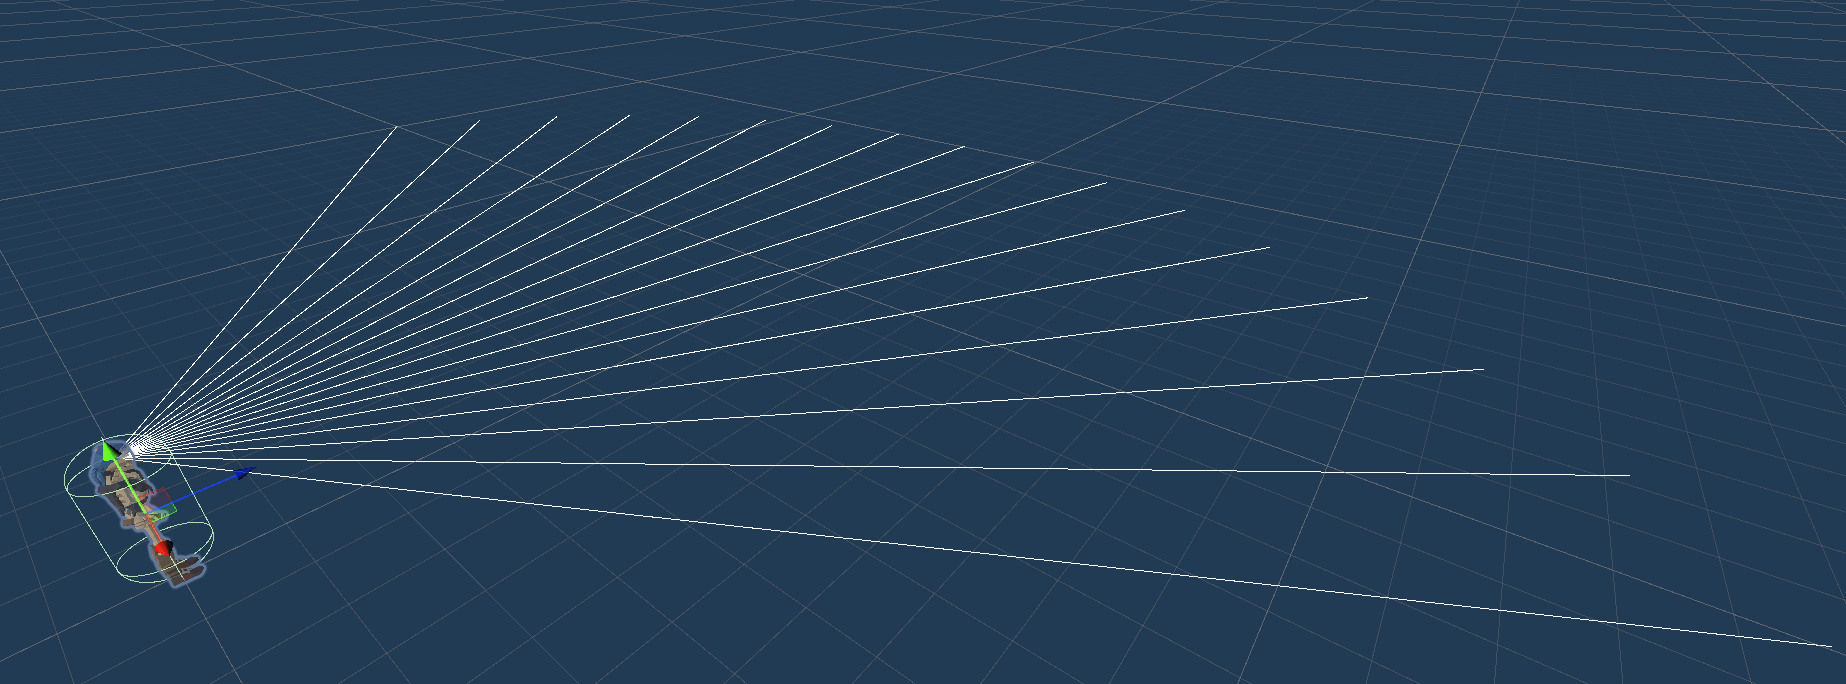
\includegraphics[width=1\textwidth]{Figures/rayperceptron.png}
    \caption{Zorné pole NPC agenta ovládaného reinforcement learningom}
    \label{pic:rayPercept}
\end{figure}

% Chapter 7
\chapter{Trénovanie agentov s využitím reinforcement learningu}
\label{sec:Training}
Táto kapitola si kladie za cieľ popísať proces trénovania agentov využívajúcich reinforcement learning. Pre toto trénovanie bola vytvorená špeciálna scéna, ktorá obsahuje 9 trénovacích plôch, čo umožňuje paralelizovať trénovací proces. Zároveň museli byť vyvinuté mechanizmy, ktoré umožnili automatizované trénovanie bez nutnosti opakovaného priechodu scenárom riadeným ľudským hráčom, ktorý by ani nebol schopný prechádzať viaceré scenáre naraz. Jednotlivé tréningové scenáre postupne navyšovali nároky na trénovaného agenta, nie vždy však bolo kvôli vykonaným zmenám možné využiť model z predchádzajúceho scenára, ktorý by sa iba dotrénoval. V nasledujúcich sekciách sú uvedené najvýznamnejšie tréningové scenáre, ich špecifiká, vzniknuté problémy a riešenia spolu s výsledkami daného scenára v podobe kumulatívnej odmeny agenta.


Trénovanie samotné prebieha pomocou príkazu \textit{mlagents-learn}, ktorý je nutné spustiť z príkazového riadku pred samotným spustením scény v engine Unity. Tento príkaz vytvorí python proces, ktorý dokáže komunikovať s vytvoreným prostredím, z ktorého získava trénovacie dáta pre trénovanie reinforcement learning modelu, teda optimalizuje policy za účelom maximalizácie odmeny. Príkazu \textit{mlagents-learn} je možné nastaviť rôzne parametre ako napríklad cestu k YAML súboru obsahujúcemu nastavené hodnoty hyper-parametrov, identifikátor tréningu (nemôžu sa opakovať bez použitia prepínaču \textit{--force}) či natrénovaný model z ktorého bude aktuálny model vychádzať. Voliteľne je možné nastaviť cestu k prostrediu, pokiaľ je na trénovanie využitý build a nie scéna spustená v rámci editoru \cite{mlagentLearn}.

\section{Prvý tréningový scenár}
\label{sec:FirstScenario}
Prvý tréningový scenár, ktorý je možné vidieť na obrázku \ref{pic:firstScenario} bol veľmi jednoduchý a spočíval v tom, že agent bol spolu so svojim cieľom uzavretý v malom prostredí. Narazenie agenta do okolitých stien vyústilo k nastaveniu odmeny na hodnotu -1 a ukončeniu trénovacej epizódy. Naopak, pokiaľ sa agent dostal na dosah svojho cieľa, tréningová epizóda bola ukončená s odmenou 1. Agent aj cieľ (hráčska postava) boli na začiatku epizódy umiestnení na náhodne lokácie v rámci uzavretého priestoru a hráčska postava bola nehybná. 

\begin{figure}[!htbp]
    \centering
    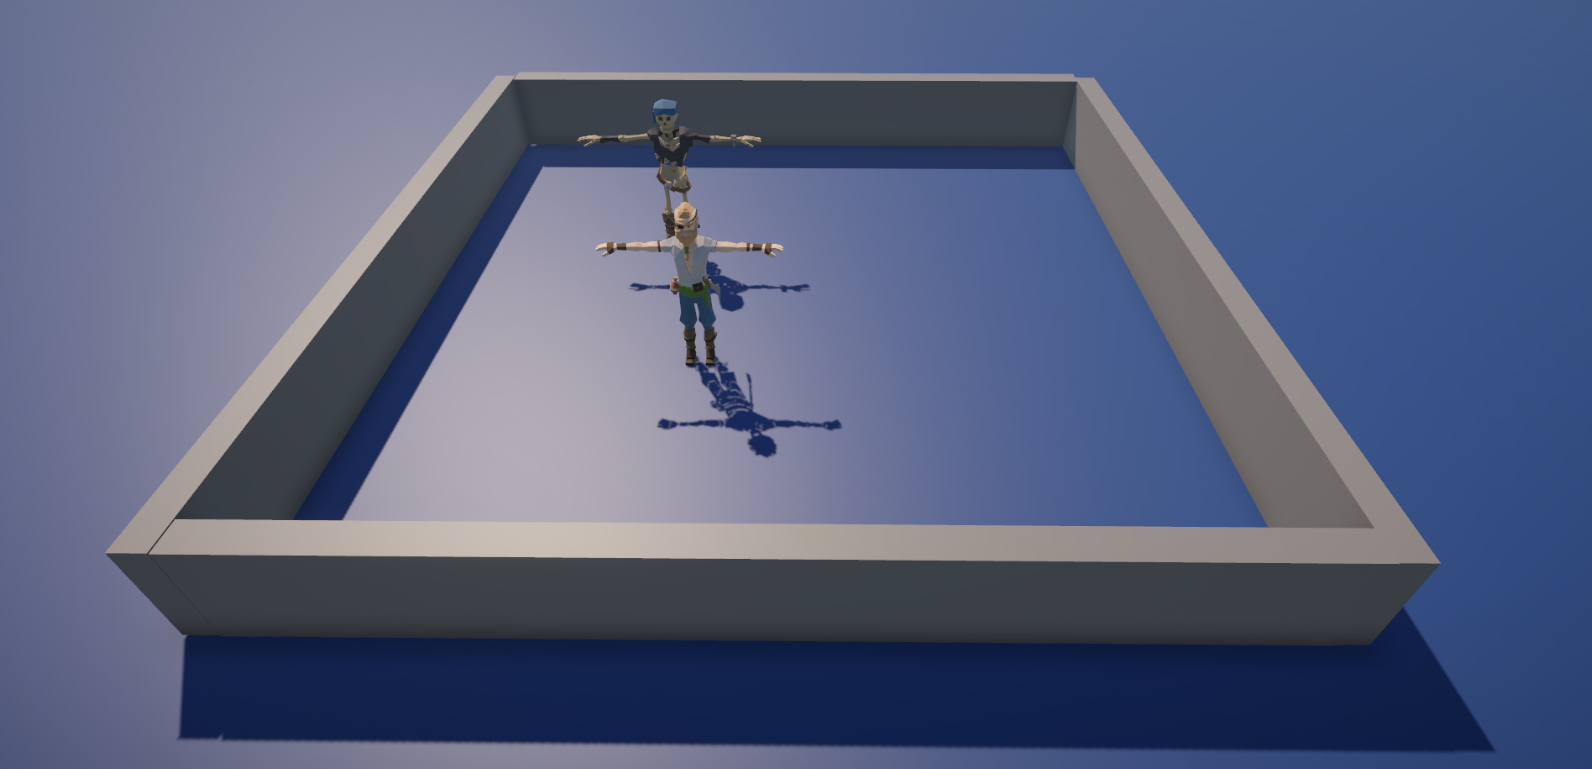
\includegraphics[width=.75\textwidth]{Figures/scenar1.png}
    \caption{Náhľad prvého tréningového scenáru}
    \label{pic:firstScenario}
\end{figure}

Agent v tomto tréningovom scenári nemal k dispozícií žiadnu percepciu. Vektor pozorovaní obsahoval 6 desatinných čísel, prvé 3 udávali lokálnu pozíciu agenta a druhé 3 lokálnu pozíciu hráčskej postavy. Tieto pozorovania boli agentovi predkladané v override metódy CollectObservations() pomocou dvoch volaní metódy AddObservation() preťaženej na Vector3, čo je známa štruktúra, ktorá v engine Unity reprezentuje 3 desatinné čísla teda pozíciu na osiach X, Y a Z. Vektor akcií agenta sa skladal z 2 kontinuálnych hodnôt, ktoré boli reprezentované ako pohyb na osiach X a Z v override metódy OnActionReceived(). Agent samozrejme nemal kontext vektoru akcií ani vektoru pozorovaní a musel sa ho naučiť metódou pokus-omyl.
Tento trénovací scenár slúžil primárne na zoznámenie sa s nástrojom ML-Agents. Ukázalo sa však, že prednastavené hyper-parametre trénovacieho algoritmu PPO boli zvolené veľmi nevhodne a agent sa nebol schopný po určitej dobe zlepšovať ani keď mal k dispozícií všetky potrebné informácie. Postupným ladením týchto parametrov za pomoci rôznych dostupných informačných zdrojov sa podarilo učenie maximálne zefektívniť. Nastavené parametre, ktoré je možné vidieť vo výpise \ref{src:params} sa ukázali byť dostatočné aj v nasledujúcich tréningových scenároch a teda nebolo potrebné ich meniť.

\vspace{8pt}
\begin{lstlisting}[language=yml,label=src:params,caption={Hyper-parametre PPO modelu využité pri tréninug NPC agenta Skeleton}]
behaviors:
  Skeleton_Agent:
    trainer_type: ppo
    hyperparameters:
      batch_size: 128
      buffer_size: 2048
      learning_rate: 0.0003
      beta: 0.01
      epsilon: 0.2
      lambd: 0.95
      num_epoch: 3
      learning_rate_schedule: linear
    network_settings:
      normalize: false
      hidden_units: 256
      num_layers: 2
      vis_encode_type: simple
    reward_signals:
      extrinsic:
        gamma: 0.99
        strength: 1.0
    keep_checkpoints: 5
    max_steps: 2000000
    time_horizon: 64
    summary_freq: 60000
\end{lstlisting}

Graf kumulatívnej odmeny modelu pri použití hyper-parametrov z výpisu \ref{src:params} je zobrazený na obrázku \ref{plt:firstScenario}. Na tomto grafe je možné vidieť, že zhruba po \(1,2 \times 10^5\) krokoch sa agent bezchybne naučil nájsť svoj cieľ a prakticky všetky ďalšie tréningové epizódy končili úspechom.

%\vspace{8pt}
\begin{figure}[!htbp]
    \centering
    \begin{tikzpicture}
        \begin{axis}[cycle list name=tb, 
%                     grid=both,
%                     grid style={solid,gray!30!white},
                     ymajorgrids=true,
                     grid style=dashed,
                     ymax=1.0, %xmax=1.3*10^5,
                     axis lines=middle,
                     xlabel={Počet krokov},
                     ylabel={Kumulatívna odmena},
                     y tick label style={/pgf/number format/.cd, fixed, fixed zerofill, precision=2, /tikz/.cd},
                     x label style={at={(axis description cs:0.5,-0.12)},anchor=north},
                     y label style={at={(axis description cs:-0.16,.5)},rotate=90,anchor=south},]
          \addplot table [x=Step, y=Value, col sep=comma] {Data/SkeletonAgentBrain1_Skeleton_Agent.csv};
        \end{axis}
    \end{tikzpicture}
    \caption{Graf kumulatívnej odmeny modelu v prvom tréningovom scenári}
    \label{plt:firstScenario}
\end{figure}

\section{Druhý tréningový scenár}
\label{sec:SecondScenario}
V druhom scenári bola rozšírená plocha po ktorej sa agent môže pohybovať. Ďalej bola odstránená stena a pohyb agenta bol obmedzený vzdialenosťou od počiatočného bodu, ktorý sa nachádzal v strede trénovacej plochy. Na začiatku epizódy majú agent aj hráčska postava vždy fixne danú pozíciu. Hráčska postava sa automaticky pohybovala z jednej strany tréningovej plochy na druhú po určených bodoch. Výber nasledujúceho bodu však prebiehal náhodne. Pre tento účel boli vytvorené dve komponenty: PlayerAutomaticMovement a ScriptedPath. Prvá spomenutá bola pridaná na hráčsku postavu spolu so spomínanou komponentou NavMeshAgent. Na tréningovej ploche bol teda vytvorený NavMesh, ktorý bol veľmi jednoduchý nakoľko tréningová plocha bola rovná a bez prekážok. Komponenta PlayerAutomaticMovement teda zabezpečovala, že keď sa hráčska postava po NavMeshi priblíži k cieľovému bodu je náhodne vybraný ďalší bod v ceste. Tento nasledujúci bod bol vždy braný z komponenty ScriptedPath, ktorá bola vytvorená na prázdnom objekte v scéne a jej podradenými objektami boli práve ručne umiestnené body na tréningovej ploche. Tieto body boli nazvané ako WayPointVariant a boli organizované do tzv. WayPointov z dôvodu, aby sa nasledujúci bod vždy vybral ako varianta najbližšieho WayPointu na ceste k cieľu, nie ľubovoľnom. Tento tréningový scenár je možné vidieť na obrázku \ref{pic:secondScenario}.

\begin{figure}[!htbp]
    \centering
    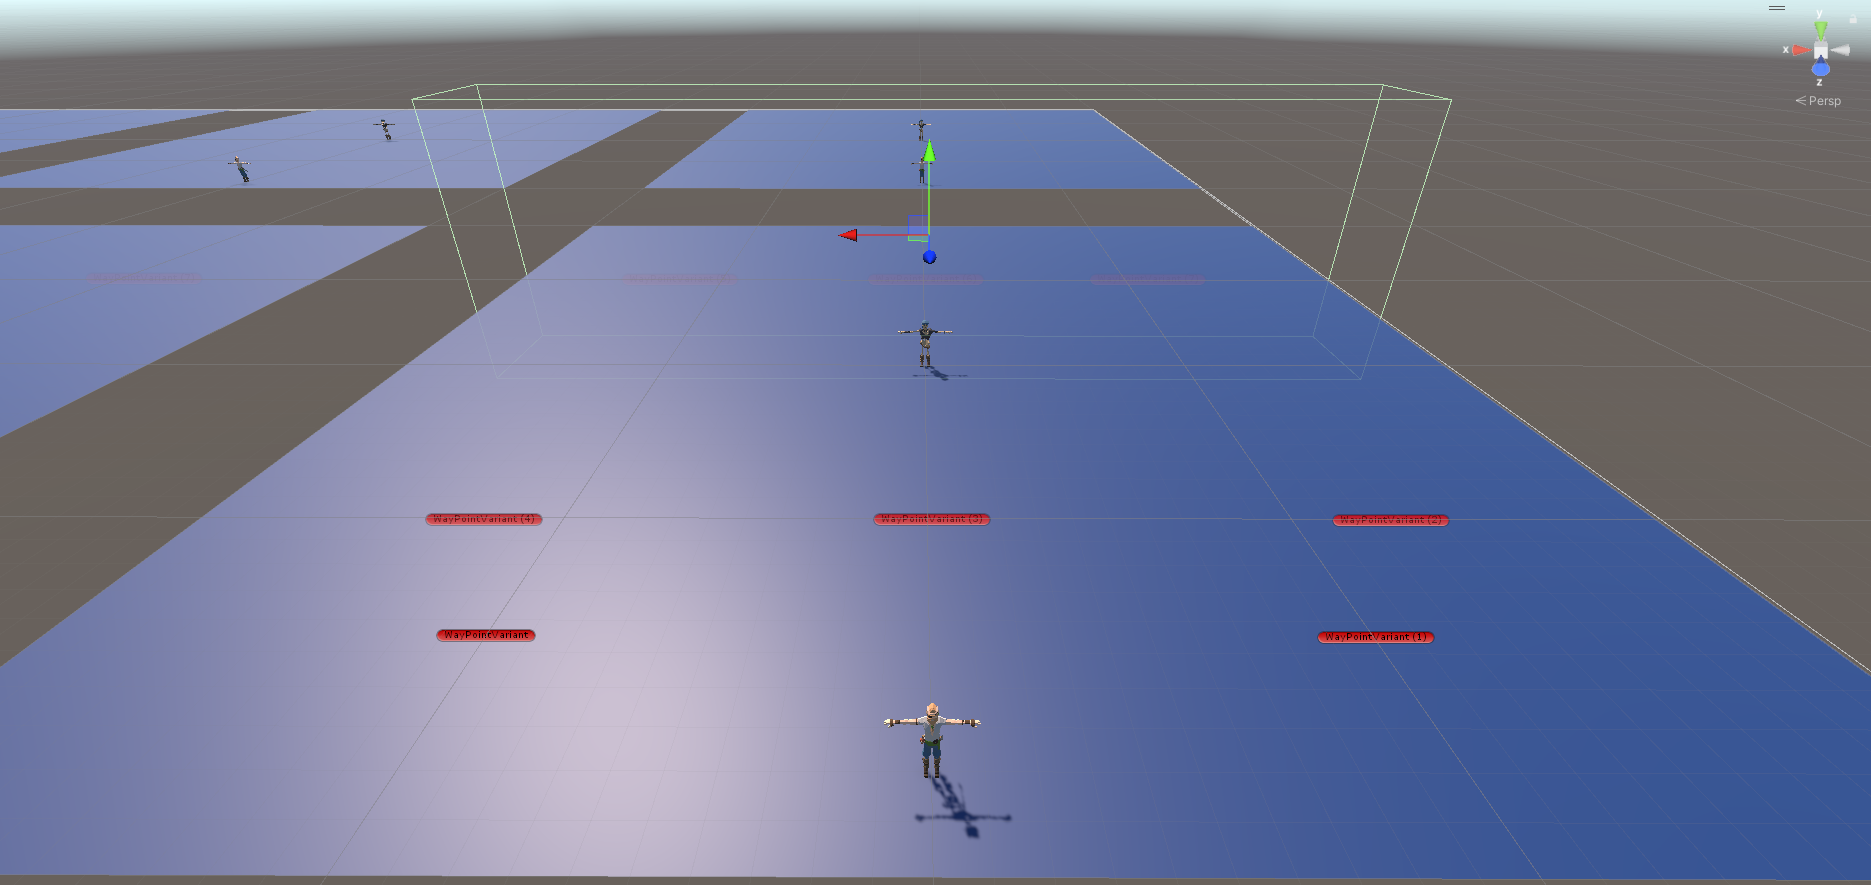
\includegraphics[width=.8\textwidth]{Figures/scenar2.png}
    \caption{Náhľad druhého tréningového scenáru}
    \label{pic:secondScenario}
\end{figure}

Na obrázku \ref{pic:secondScenario} je možné si všimnúť jednotlivé body, z ktorých hráčska postava vyberá nasledujúci a objekt Finish v podobe zeleného Collideru, ktorý pri strete s hráčskou postavou ukončí epizódu neúspechom pre agenta. Zmena nastala aj v prípade odmeňovania agenta, kedy za úspešnú epizódu bol pridaný (nie nastavený) 1 bod odmeny a za neúspešnú epizódu bol 1 bod odmeny odobratý. Zvyšné parametre ako vektor akcií či pozorovaní agenta ostali nezmenené. Vývoj kumulatívnej odmeny pre tento scenár je možné vidieť v grafe \ref{plt:secondScenario}. Pri systéme odmeňovania -1, +1 však tento graf znázorňuje úspešnosť okolo 40\%. Navyšovanie počtu krokov viedlo iba k stagnácií modelu.

%\vspace{8pt}
\begin{figure}[!htbp]
    \centering
    \begin{tikzpicture}
        \begin{axis}[cycle list name=tb, 
%                     grid=both,
%                     grid style={solid,gray!30!white},
                     ymajorgrids=true,
                     grid style=dashed,
                     ymax=40.0, xmax=3*10^5,
                     axis lines=middle,
                     xlabel={Počet krokov},
                     ylabel={Kumulatívna odmena},
                     y tick label style={/pgf/number format/.cd, fixed, fixed zerofill, precision=2, /tikz/.cd},
                     x label style={at={(axis description cs:0.5,-0.12)},anchor=north},
                     y label style={at={(axis description cs:-0.19,.5)},rotate=90,anchor=south},]
          \addplot table [x=Step, y=Value, col sep=comma] {Data/SkeletonAgentBrain3_Skeleton_Agent.csv};
        \end{axis}
    \end{tikzpicture}
    \caption{Graf kumulatívnej odmeny modelu v druhom tréningovom scenári}
    \label{plt:secondScenario}
\end{figure}

\section{Tretí tréningový scenár}
\label{sec:ThirdScenario}
Nakoľko výsledky predchádzajúceho scenáru boli slušné ale nie úplne dostačujúce, v treťom scenári bol upravený systém odmeňovania. Agent za úspešný stret so svojim cieľom dostal 100 bodov odmeny a za neúspešnú epizódu (keď sa hráčska postava dostala do cieľa alebo agent vyšiel mimo stanovenú trénovaciu plochu) dostal penalizáciu v podobe 10 bodov. Zároveň mu bola kontinuálne udeľovaná malá penalizácia, čo ho malo ešte viac podnietiť k riskantnému chovaniu v snahe dohnať svoj cieľ v čo najkratšom čase. 

Agent s takto upraveným systémom odmien však stále nedosahoval kýžených výsledkov. Tie dosiahla až zmena vektoru pozorovaní z pôvodných 6 desatinných čísel (2x Vector3), reprezentujúcich pozíciu agenta a cieľa, na 3 desatinné čísla (1x Vector3), ktoré reprezentujú relatívnu pozíciu cieľa voči agentovi. Výpočet tejto relatívnej pozície je možné vidieť vo výpise \ref{src:GetRelativePosition}.

\vspace{8pt}
\begin{lstlisting}[label=src:GetRelativePosition,caption={Získavanie reltívnej pozície cieľa voči agentovi}]
public static Vector3 GetRelativePosition(Transform origin, Vector3 position)
{
    Vector3 distance = position - origin.position;
    Vector3 relativePosition = Vector3.zero;
    relativePosition.x = Vector3.Dot(distance, origin.right.normalized);
    relativePosition.y = Vector3.Dot(distance, origin.up.normalized);
    relativePosition.z = Vector3.Dot(distance, origin.forward.normalized);
    return relativePosition;
}
\end{lstlisting}

Kumulatívnu odmenu po týchto zmenách je možné vidieť v grafe \ref{plt:thirdcenario}.

%\vspace{8pt}
\begin{figure}[!htbp]
    \centering
    \begin{tikzpicture}
        \begin{axis}[cycle list name=tb, 
%                     grid=both,
%                     grid style={solid,gray!30!white},
                     ymajorgrids=true,
                     grid style=dashed,
                     ymax=90.0, %xmax=3*10^5,
                     axis lines=middle,
                     xlabel={Počet krokov},
                     ylabel={Kumulatívna odmena},
                     y tick label style={/pgf/number format/.cd, fixed, fixed zerofill, precision=2, /tikz/.cd},
                     x label style={at={(axis description cs:0.5,-0.12)},anchor=north},
                     y label style={at={(axis description cs:-0.19,.5)},rotate=90,anchor=south},]
          \addplot table [x=Step, y=Value, col sep=comma] {Data/SkeletonAgentBrain3.5_Skeleton_Agent.csv};
        \end{axis}
    \end{tikzpicture}
    \caption{Graf kumulatívnej odmeny modelu v treťom tréningovom scenári}
    \label{plt:thirdcenario}
\end{figure}

\section{Štvrtý trénovací scenár}
\label{sec:FourthScenario}
Výsledky tretieho trénovacieho scenára boli uspokojivé a tak sa mohlo prejsť na ďalší krok. Informácia o relatívnej polohe cieľa bola nahradená využitím komponenty Ray Perception Sensor 3D, čím odpadla nutnosť ručne agentovi posielať nejaký druh informácie a vektor pozorovaní je v tomto scenári prázdny. Na základe testovania sa taktiež zistilo, že agent po nahradení kontinuálnych akcií za diskrétne dosahuje lepších výsledkov. Toto však platí len v prípade kedy vektor akcií ma veľkosť 1 a táto jedna akcia môže nadobúdať 7 stavov. V testovacích scenároch kedy boli využité 3 diskrétne akcie agent podával relatívne slabé výsledky pri trénovaní. Mapovanie diskrétnej akcie na pohyb a zmenu rotácie agenta je možné vidieť vo výpise \ref{src:MoveAgent}. V tomto výpise je možné si povšimnúť, že pohyb agenta bol realizovaný fyzikálne pomocou komponenty RigidBody. Tento prístup sa však v ďalších scenároch ukázal ako nevhodný a bol nahradený tradičným prístupom, mapovanie akcie však ostalo zachované.

Po otestovaní funkčnosti tohto riešenia boli pridané do scenára aj prekážky, ktoré agentovi mali aktívne brániť vo výhľade. Tie je možné vidieť na obrázku \ref{pic:fourthScenario}. Jednotlivé prekážky sú na začiatku každej epizódy náhodne rozmiestnené po tréningovej ploche, tak aby nezasahovali do jednotlivých aktérov. Po každom takomto rozmiestnení musel byť aktualizovaný NavMesh, aby automaticky ovládaný hráč nemohol týmito prekážkami prejsť. Náraz agenta do prekážky potom spôsobil ukončenie epizódy s penalizáciou 10 bodov. Ak sa agent priblížil na dosah svojmu cieľu dostal odmenu vo forme 100 bodov a za každý krok dostal malú penalizáciu danú výpočtom \(-1 / MaxSteps\) rovnako ako v treťom tréningovom scenári.

\vspace{8pt}
\begin{lstlisting}[label=src:MoveAgent,caption={Mapovanie diskrétnej akcie na pohyb a rotáciu agenta}]
public void MoveAgent(ActionSegment<int> act)
{
    var direction = Vector3.zero;
    var rotation = Vector3.zero;

    var action = act[0];

    switch (action)
    {
        case 1:
            direction = transform.forward * 1f;
            break;
        case 2:
            direction = transform.forward * -1f;
            break;
        case 3:
            rotation = transform.up * 1f;
            break;
        case 4:
            rotation = transform.up * -1f;
            break;
        case 5:
            direction = transform.right * -0.75f;
            break;
        case 6:
            direction = transform.right * 0.75f;
            break;
    }

    transform.Rotate(rotateDir, Time.fixedDeltaTime * rotationSpeed);
    rigidbody.AddForce(dirToGo * body.Speed, ForceMode.VelocityChange);
}
\end{lstlisting}

Kumulatívnu odmenu je opäť možné vidieť v grafe \ref{plt:fourthcenario}. Tréningové výsledky agenta síce nedosahujú výsledkov predchádzajúceho scenáru ale agent sa musí navigovať v náročnejšom prostredí, kde náraz znamená koniec epizódy a je odkázaný iba na svoj zrakový vnem. To agenta núti prehľadávať okolie, aby svoj cieľ dostal čo možno najrýchlejšie do svojho zorného poľa. 

\begin{figure}[!htbp]
    \centering
    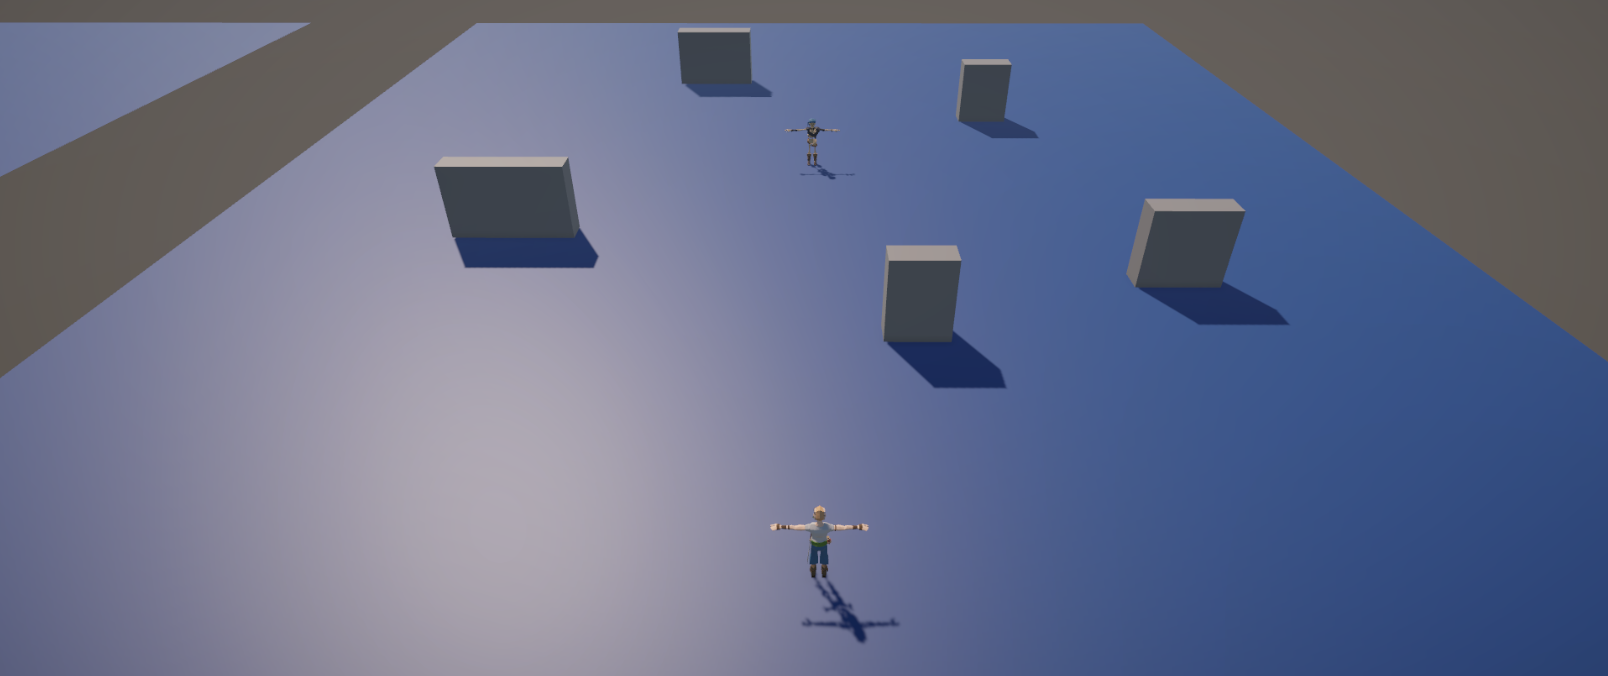
\includegraphics[width=1\textwidth]{Figures/scenar4.png}
    \caption{Náhľad štvrtého tréningového scenáru}
    \label{pic:fourthScenario}
\end{figure}

V tomto scenári mali agent aj hráčska postava veľmi podobnú rýchlosť pohybu. Keď sa však agent rozbehol po svojom cieli a ten náhle zmenil smer pohybu, agent ho vo väčšine prípadov nedokázal dohnať skôr, ako sa hráčska postava dostala do cieľa. Začína sa tu objavovať chovanie, ktoré bolo zachované aj vo finálnom modeli. Konkrétne ide o to, že agent sa snaží čo najskôr dostať svoj cieľ do zorného poľa, a keď sa mu to podarí, volí skôr taktiku vyčkávania namiesto náhleho útoku. A to aj za cenu malej penalizácie v podobe zvýšeného počtu vykonaných krokov. 

%\vspace{8pt}
\begin{figure}[!htbp]
    \centering
    \begin{tikzpicture}
        \begin{axis}[cycle list name=tb, 
%                     grid=both,
%                     grid style={solid,gray!30!white},
                     ymajorgrids=true,
                     grid style=dashed,
                     ymax=90.0, xmax=5*10^5,
                     axis lines=middle,
                     xlabel={Počet krokov},
                     ylabel={Kumulatívna odmena},
                     y tick label style={/pgf/number format/.cd, fixed, fixed zerofill, precision=2, /tikz/.cd},
                     x label style={at={(axis description cs:0.5,-0.12)},anchor=north},
                     y label style={at={(axis description cs:-.19,.5)},rotate=90,anchor=south},]
          \addplot table [x=Step, y=Value, col sep=comma] {Data/SkeletonAgentBrain4.2_Skeleton_Agent.csv};
        \end{axis}
    \end{tikzpicture}
    \caption{Graf kumulatívnej odmeny modelu krokov vo štvrtom tréningovom scenári}
    \label{plt:fourthcenario}
\end{figure}

\section{Finálny trénovací scenár}
\label{sec:FinalScenario}
Na výsledkoch predchádzajúceho scenáru bolo do veľkej miery možné stavať. Oproti nemu však agent aj prostredie prešlo niekoľkými iteratívnymi zmenami. Agentovi bol pridaný aj druhý zmysel, a síce počutie. Realizácia počutia musela byť mierne odlišná od tej využívanej pri druhom type agenta aj keď komponenta Hearing ostala nezmenená. Agentovi bol navrátený vektor pozorovaní o veľkosti 3 desatinných čísel a jedného príznaku. Prvé 3 čísla označujú relatívnu pozíciu posledného zdroja zvuku voči agentovi. Tá bola získaná štandardným spôsobom z komponenty Hearing. Nakoľko však nie je možné odoslať do rozhodovacieho procesu informáciu v rámci reakcie na event, ale iba v periodickom volaní metódy AddObservation() v rámci override metódy CollectObservations(), je spolu s relatívnou pozíciou k poslednému zdroju zvuku odosielaný aj príznak. Ten pomáha agentovi určiť, či ide o reálny zdroj zvuku alebo iba inicializačnú hodnotu v prípade, že žiadny relevantný zvuk v okolí nenastal. 

Vďaka pridaniu nového vnemu sa agent prestal toľko zameriavať na správnu rotáciu k svojmu cieľu a v niektorých trénovacích epizódach sa stávalo, že agent dohnal hráčsku postavu akoby pozadu. Toto by šlo kompenzovať viacerými spôsobmi ako napríklad obmedzením rýchlosti cúvania. Nakoľko však agent ovládaný rozhodovacím stromom môže na hráča útočiť iba keď ho vidí, bola táto podmienka zavedená aj pri tomto type agenta. 

Systém odmeňovania ostal nezmenený, nakoľko sa osvedčil. Malá zmena nastala v pohybe agenta, kedy bol fyzikálny systém využitý v predchádzajúcom scenári nahradený za štandardný spôsob pomocou metódy Translate() a to v globálnej súradnicovej sústave. Všetky predchádzajúce scenáre využívali na pohyb lokálnu súradnicovú sústavu, teda relatívnu voči svojmu predkovi v scéne. Tento systém fungoval v poriadku iba do momentu reálneho nasadenia agenta do hernej scény. V nej sa agent totiž stále snažil dostať na súradnice, ktoré sa nachádzali ďaleko od jeho zamýšľaného stanoviska, a síce uprostred oceánu.

Posledný problém, ktorý sa vyskytol pri pokusoch o reálne nasadenie agenta v hernej scéne, spočíval v tom, že agent bol natrénovaný na to, že hráčska postava chodí iba z jedného smeru a tento smer mal dokonale pokrytý. Ak však hráč prichádzal z iného smeru, agent naňho len zriedka adekvátne zareagoval. Do tréningovej plochy, ktorá inak ostala nezmenená od posledného scenára, bola pridaná rotácia prekážok a hráčskej postavy spolu s jej cieľom. Na začiatku každej epizódy sa teda náhodne vygenerovala počiatočná pozícia hráčskej postavy na jednej hrane štvorcovej trénovacej plochy a na opačnú hranu bol umiestnený cieľ pre túto postavu. Agent teda v momente, v ktorom zachytil hráčsku postavu jedným zo zmyslov, nevedel, z ktorého smeru táto postava ide, ani kde sa nachádza jej cieľ.

Vďaka konzistentnosti vo vektore pozorovaní či ustálenému spôsobu pohybu už bolo možné pri jednotlivých iteratívnych zmenách model tzv. dotrénovať a nebolo nutné vždy začínať s úplne novým. Kumulatívna odmena pre tento scenár zobrazená na grafe \ref{plt:finalScenario} teda reprezentuje už len toto dotrénovanie a finálna úspešnosť modelu sa teda pohybuje niekde pri hranici 87 bodov, čo považujeme za veľmi dobrú hodnotu vzhľadom na špecifiká trénovacieho scenára. Tieto hodnoty by bolo možné navyšovať napríklad zvyšovaním rýchlosti agenta či znižovaním rýchlosti hráča, prípadne úpravou trénovacej oblasti, aby mal agent viac času na analyzovanie situácie. V úzkych koridoroch by napríklad hráč bez možnosti brániť sa nemal proti takémuto agentovi šancu. Nejaké zmeny v rýchlostiach jednotlivých aktérov boli skutočne ešte dodatočne vykonané ale s dôrazom na vyváženie obtiažnosti hry, nie na zvyšovanie úspešností agenta. 
%\vspace{8pt}
\begin{figure}[!htbp]
    \centering
    \begin{tikzpicture}
        \begin{axis}[cycle list name=tb, 
%                     grid=both,
%                     grid style={solid,gray!30!white},
                     ymajorgrids=true,
                     grid style=dashed,
                     ymax=90.0, %xmax=3*10^5,
                     axis lines=middle,
                     xlabel={Počet krokov},
                     ylabel={Kumulatívna odmena},
                     y tick label style={/pgf/number format/.cd, fixed, fixed zerofill, precision=2, /tikz/.cd},
                     x label style={at={(axis description cs:0.5,-0.12)},anchor=north},
                     y label style={at={(axis description cs:-.19,.5)},rotate=90,anchor=south},]
          \addplot table [x=Step, y=Value, col sep=comma] {Data/SkeletonAgentBrain6.6_Skeleton_Agent.csv};
        \end{axis}
    \end{tikzpicture}
    \caption{Graf kumulatívnej odmeny modelu vo finálnom tréningovom scenári}
    \label{plt:finalScenario}
\end{figure}

%TODO + PlayerAutomatic movement, scriptedPath, waypointy, navmesh - len ze uz bol vysvetleny
% trenovacie scenare a grafy z treningu, parametre

% Chapter 8
\chapter{Porovnanie implementovaných prístupov}
\label{sec:Compare}
Táto kapitola je venovaná porovnaniu využitých algoritmov machine learningu. Jednotlivé algoritmy určené na vytváranie rozhodovacieho stromu boli porovnané z hľadiska času tejto konštrukcie a z hľadiska ich výstupov. U algoritmu PPO ako zástupcu triedy reinforcement learningu boli zaznamenané údaje o dĺžke trénovacej epizódy. Porovnaniu z hľadiska výkonu bolo podrobené aj vykonávanie rozhodnutí, či už na základe rozhodovacieho stromu alebo naučeného modelu. V závere kapitoly sú potom uvedené poznatky založené na empirickom pozorovaní rozdielov v chovaní jednotlivých typov NPC a diskusia týchto výsledkov.

Všetky výkonnostné testy boli vykonané na zostave, s nasledujúcimi parametrami:
\begin{itemize}
    \item \textbf{Procesor} -- AMD Ryzen 9 5900X
    \begin{itemize}
        \item \textbf{Počet jadier} -- 12
        \item \textbf{Počet vláken} -- 24
        \item \textbf{Frekvencia} -- 3,7GHz (4,8GHz)
    \end{itemize}
    \item \textbf{Grafická karta} -- GAINWARD GeForce RTX 3070 Ti Phoenix
    \begin{itemize}
        \item \textbf{Veľkosť grafickej pamäte} -- 8GB
        \item \textbf{Frekvencia grafického procesoru} -- 1575MHz (1785MHz)
    \end{itemize}
    \item \textbf{Pamäť RAM} -- Crucial Ballistix Red 32GB (4x8GB)
    \begin{itemize}
        \item \textbf{Typ pamäte} -- DDR4
        \item \textbf{Frekvencia} -- 3600MHz
        \item \textbf{Časovanie} -- CL16 (16-18-18-38)
    \end{itemize}
    \item \textbf{Disk} -- Samsung 980 1TB
    \begin{itemize}
        \item \textbf{Rozhranie} -- M.2 (PCIe 3.0 4x NVMe)
    \end{itemize}
\end{itemize}

\section{Porovnanie výkonu jednotlivých algoritmov pri učení}
\label{sec:id3d45cart}
Výkon algoritmov určených na tvorbu rozhodovacieho stromu bol porovnaný na dátovej sade, ktorú je možné vidieť v tabuľke \ref{tab:skeletonActionRaw}. Každý algoritmus bol spustený 1000x aby sa zamedzilo náhodným odchýlkam v testovaní. Výsledky v podobe najkratšieho, priemerného a najdlhšieho času nutného na spracovanie vstupných dát do rozhodovacieho stromu sú uvedené v tabuľke \ref{tab:benchmarks}.

\begin{table}[!ht]
    \centering
    \begin{tabular}{|c|ccc|}
    \hline
        \textbf{Algoritmus} & \textbf{Minimálny čas [ms]} & \textbf{Priemerný čas [ms]} & \textbf{Maximálny čas [ms]} \\ \hline
        \textbf{ID3} & 106.989 & 109.559 & 120.763 \\ 
        \textbf{D4.5} & 39.976 & 41.415 & 75.001 \\ 
        \textbf{CART} & 21.787 & 23.673 & 37.998 \\ \hline
    \end{tabular}
    \caption{Porovnanie času spracovania vstupných dát algoritmami ID3, D4.5 a CART}
    \label{tab:benchmarks}
\end{table}

Z tabuľky je možné jasné vidieť, že najlepšie dopadol algoritmus CART, druhý bol algoritmus D4.5 a najhoršie výsledky z hľadiska výkonu dosahoval algoritmus ID3. Na tieto výsledky je však nutné pozerať sa v kontexte výstupov jednotlivých algoritmov. Výstup oboch algoritmov D4.5 a CART bol totožný a naozaj odpovedal najoptimálnejšiemu rozhodovaciemu stromu, aký je možné z danej dátovej sady vytvoriť. Grafickú reprezentáciu tohto výstupu je možné vidieť na obrázku \ref{pic:treeGraph}.

\begin{figure}[!htbp]
    \centering
    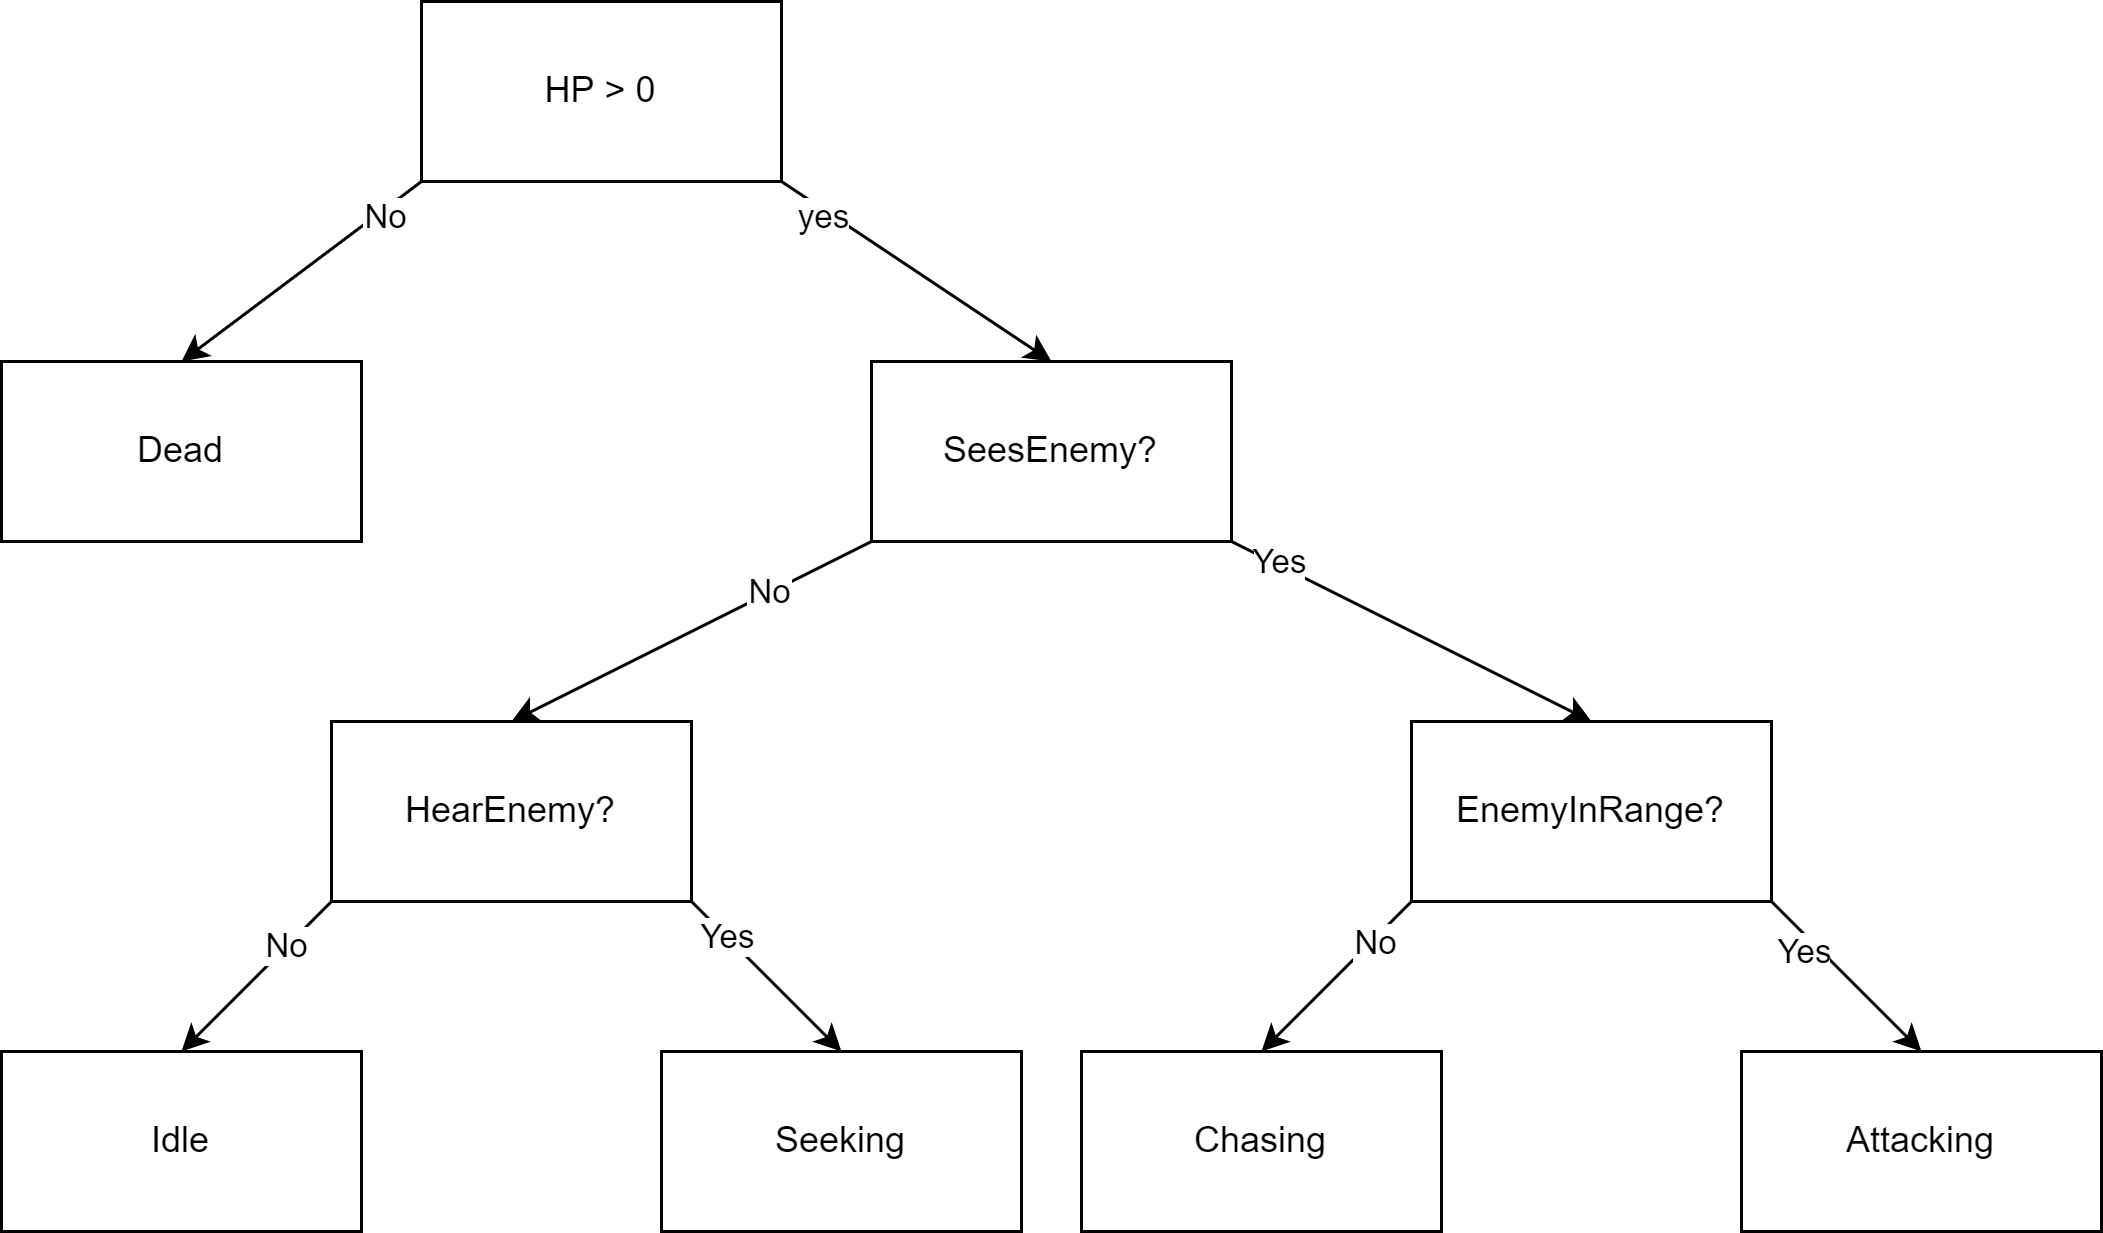
\includegraphics[width=1\textwidth]{Figures/Trees.png}
    \caption{Rozhodovací strom vytvorený algoritmami D4.5 a CART}
    \label{pic:treeGraph}
\end{figure}

Rozdiel v čase trvania algoritmu CART v porovnaní s D4.5 je potom daný jedinou využívanou metrikou algoritmu CART pri konštrukcií rozhodovacieho stromu, a síce Gini indexom. V prípade, že by výstup algoritmov ID3 a D4.5 bol totožný, je predpoklad, že časy trvania by boli veľmi podobné a dokonca v prospech algoritmu ID3. Ten však v danej dátovej sade nedokázal nájsť najoptimálnejšie rozdelenie a teda musel vykonať viac krokov. Výsledkom je rozhodovací strom, ktorý má viac vrcholov ako by bolo nutné a zároveň umožňuje vstup do listu Seeking aj v prípade, že zdravie agenta tomu neodpovedá. Aby však vôbec algoritmus ID3 mohol byť na daných dátach porovnaný s ostatnými, musela byť jeho implementácia obohatená o možnosť spracovať kontinuálne hodnoty pomocou operátorov <= a >. Túto schopnosť štandardne algoritmus ID3 nemá a s tým súvisia aj dané problémy. Grafickú reprezentáciu rozhodovacieho stromu vytvorenú týmto algoritmom je možné vidieť na obrázku \ref{pic:treeGraphID3}.

\begin{figure}[!htbp]
    \centering
    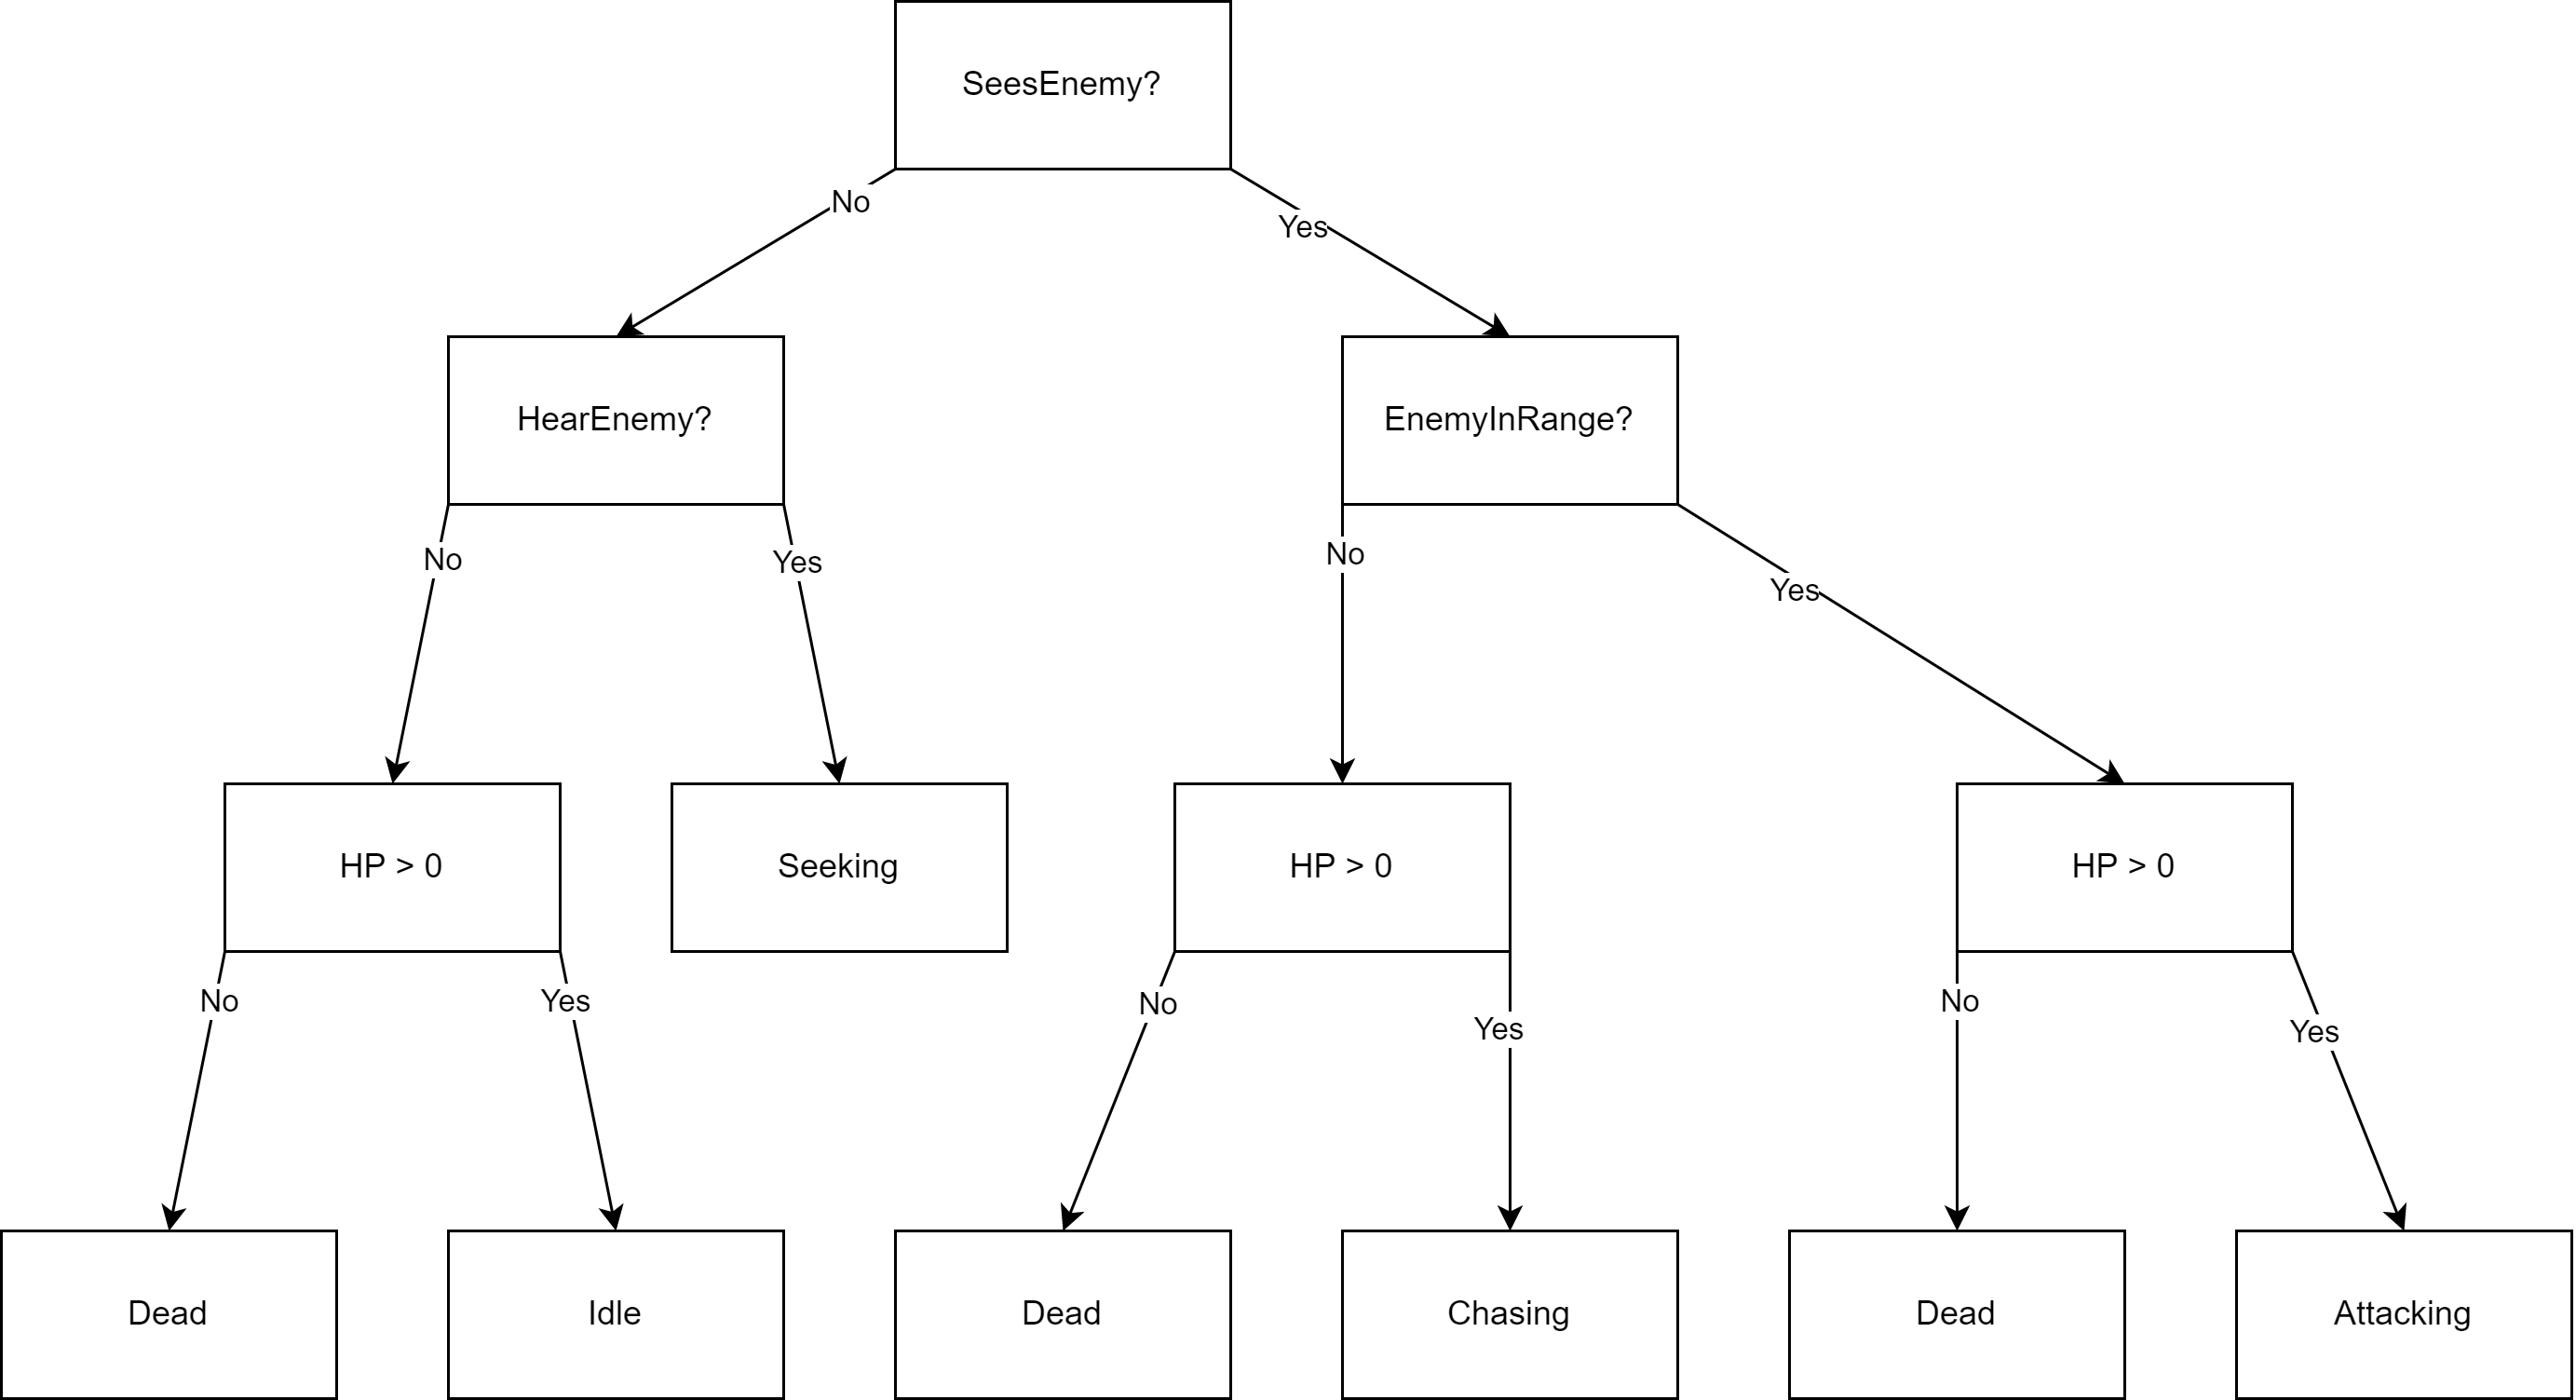
\includegraphics[width=1\textwidth]{Figures/idTree.png}
    \caption{Rozhodovacieho strom vytvorený algoritmom ID3}
    \label{pic:treeGraphID3}
\end{figure}

Časy uvedené v tabuľke \ref{tab:benchmarks} je možné dať do kontextu aj s reinforcement learning algoritmom PPO. Priemerný čas nutný na vykonanie 1000 tréningových krokov, pri simultánnom trénovaní 9 agentmi, nameraný na vzorke 1,2 milióna krokov bol 15004,994ms, teda okolo 15 sekúnd. K dosiahnutiu uspokojivého výsledku však agent musel vykonať stovky tisíc až jednotky miliónov krokov. Toto je samozrejme násobne viac ako je trvanie vytvorenie jedného rozhodovacieho stromu. Treba však brať do úvahy, že algoritmus na tvorbu rozhodovacieho stromu má testovacie dáta vopred pripravené. Z pohľadu strojového učenia obecne však hodnotu 15 sekúnd na vykonanie 1000 tréningových krokov považujeme na danom HW za veľmi slušnú, nakoľko v rámci jednotiek minút je možné natrénovať schopný model, ktorý dokáže vykonávať základné úkony popisované v tomto projekte. V praxi to znamená, že s danými nástrojmi a HW je možné dosiahnuť efektívny iteratívny vývoj pomocou ladenia hyper-parametrov, úpravou prostredia či vlastností a vnútornej logiky agenta. 

\section{Porovnanie výkonu jednotlivých algoritmov pri rozhodovaní}
\label{sec:editorPerformance}
Ako, už bolo spomenuté, jednotlivé algoritmy boli porovnané aj z hľadiska výkonu pri rozhodovaní. Výsledky boli namerané v samostatnom builde pri vypnutej vertikálnej synchronizácií. Ako metrika bola zvolená priemerná hodnota FPS popisovaná v sekcií \ref{sec:GameLoop}. Nakoľko algoritmy CART a D4.5 vytvorili identický rozhodovací strom, ich výsledky boli zlúčené. 

Testovanie prebiehalo vo viacerých scenároch. Prvým bola prázdna scéna. Tento scenár mal demonštrovať maximálnu priemernú hodnotu FPS na akú je možné sa na danom HW s danými nastaveniami grafiky dostať. Následne boli porovnané medzi sebou jednotlivé algoritmy. Scéna v tomto prípade obsahovala 30 agentov, ktorí mali vypnuté vykresľovanie modelov a hráčsku postavu. Namerané výsledky je možné vidieť v tabuľke \ref{tab:benchmarksGame}.

\begin{table}[!ht]
    \centering
    \begin{tabular}{|l|c|}
    \hline
        \textbf{Scenár} & \textbf{Priemerná hodnota FPS} \\ \hline
        Prázdna scéna & 628,81 \\ 
        D4.5, CART & 602,46 \\ 
        ID3 & 605,34 \\ 
        PPO & 598,75 \\ \hline
    \end{tabular}
    \caption{Porovnanie priemernej hodnoty FPS pri rozhodovaní}
    \label{tab:benchmarksGame}
\end{table}

Z nameraných hodnôt je možné si všimnúť, že rozdiel medzi priemernou hodnotou FPS v prázdnej scéne a s aktívnymi agentmi sa pohybuje medzi 19-30 FPS, čo za daných okolností nie je prekvapujúce. Rozdiely medzi algoritmami D4.5, CART a ID3 sú malé, dokonca mierne v prospech stromu vytvoreného algoritmom ID3. Rozdiel medzi priemernou hodnotu FPS reinforcement learning algoritmu PPO a zvyšných algoritmov taktiež neukázal žiadne výrazné výkyvy. Úzkym hrdlom vo všetkých prípadoch bol procesor, nakoľko vykresľovanie 3D modelov jednotlivých agentov bolo vypnuté. 

\section{Empirické porovnanie a diskusia výsledkov}
\label{sec:Discussion}
Všetky otestované metódy je teda možné z hľadiska výkonu využiť aj v reálnom nasadení. Pri praktickom nasadení by vykresľovanie 3D modelov jednotlivých agentov aj ich rozhodovanie podliehalo určitej implementácií LOD systému, ktorý by úplne zakázal, či aspoň výrazne obmedzil vykresľovanie modelov, ktoré sú vzdialené alebo za prekážkou. Pokiaľ by bolo nutné v hre vykresľovať desiatky NPC naraz a tento spôsob by nedostačoval, je možné použiť aj sofistikovanejšie metódy ako napríklad systém DOTS v engine Unity. Obdobu LOD systému je možné aplikovať aj na samotné rozhodovanie, kedy nie je nutné, aby NPC, ktoré je vzdialené od hráča vykonávalo rozhodovací proces periodicky v rámci desatín sekúnd alebo dokonca menej. V závislosti od úrovne simulácie je možné na takýchto NPC rozhodovanie aj úplne zamedziť. Z tohto dôvodu bola využitá korutina, ktorej časové oneskorenie je možné ladiť a nie napríklad metóda Update(). Ak by opäť nedostačoval ani tento systém, je možné siahnuť napríklad po implementácií rozhodovania zdieľaného medzi rôznymi inštanciami akú využívajú napríklad behaviorálne stromy v engine Unreal. Možností optimalizácie je samozrejme veľké množstvo.

Po stránke výkonu sú si síce jednotlivé prístupy veľmi podobné, existujú však značné rozdiely v chovaní jednotlivých NPC a celkovo aj v náročnosti tvorby určitého chovania či jeho neskoršieho adaptovania. Výhodou využitia rozhodovacích stromov je nižšia náročnosť a viac priamočiara metodika ich tvorby. Zároveň umožňujú dynamicky meniť či upravovať chovanie jednotlivých NPC bez nutnosti kompilácie kódu či buildu celého projektu. Vytvorenie dátovej sady pre daný typ úlohy nie až tak náročné ale veľmi samozrejme záleží na komplexnosti celého chovania. Spracovanie dát algoritmom je veľmi rýchla operácia, ktorej výsledok je možné okamžite pozorovať na výstupe ešte pred nasadením do hry. Rozhodovací strom sa však, ako jeho názov napovedá, zaoberá iba rozhodovacím procesom, nie chovaním agenta, ktoré nasleduje po vykonaní rozhodnutia. 

Naproti tomu, algoritmy reinforcement learningu sa zaoberajú chovaním agenta obecne. Natrénovaný model sa dokáže sám navigovať prostredím pomocou percepcie a jeho chovanie môže byť veľmi komplexné. Príkladom môže byť napríklad to, akým spôsobom agent reaguje na hráča. Nerozbehne sa hneď po ňom, ale vyčkáva, čo hráč urobí a ktorým smerom pôjde. Toto chovanie je pochopiteľné a približuje sa tomu, ako by sa v danej situácií choval ľudský hráč. Naprogramovať však takéto chovanie nie je triviálnym úkonom. To však nie je ani natrénovanie agenta pomocou reinforcement learningu. Táto obtiažnosť navyše prudko narastá s komplexnosťou danej úlohy. Chovanie umelej inteligencie v dnešných hrách sa často skladá z viacerých vrstiev a natrénovať takého agenta by bolo veľmi zložité. Riešením by mohlo byť natrénovanie viacerých modelov určených na konkrétne úkony a ich prepínanie podľa potreby alebo rôzne hybridné prístupy. Herní vývojári taktiež chcú mať nad chovaním NPC čo najväčšiu kontrolu, aby hráčovi zabezpečili optimálny herný zážitok. Napriek tomu, že agentove správanie v niektorých situáciach pripomína správanie hráča, v iných by sa len ťažko zlučovalo s dnešnou snahou o imerziu a realistickosť, akú sa dnešné hry snažia docieliť. Nehovoriac o tom, že herný vývoj je iteratívny proces a každá zmena herného dizajnu súvisiaceho s NPC by mohla znamenať nutnosť model upraviť či vytrénovať nanovo. Problémom by mohla byť aj obtiažnosť takýchto hier a jej úprava.

% Chapter 9
\chapter{Záver}
\label{sec:Conclusion}
V rámci tejto diplomovej práce sa podarilo vytvoriť herné 3D prostredie v engine Unity s využitím programovacieho jazyka C\#, v ktorom sú na rozhodovanie NPC využité rôzne algoritmy z oblasti strojového učenia. Toto prostredie je zasadené do pirátskej tematiky a obsahuje hernú slučku, v ktorej sa hráč môže voľne pohybovať po ostrove s plne funkčnou kamerou z pohľadu tretej osoby. Hráč môže pri preskúmavaní prostredia spomaliť svoj pohyb, aby na seba neupútal pozornosť či vykonať skok v súlade so simuláciou gravitácie. V hernom prostredí sa nachádzajú rôzne predmety, ktoré hráč môže zbierať a ich určitý počet je vyžadovaný na úspešne dokončenie hry. Hra samotná potom obsahuje aj ďalšie prvky ako napríklad hlavnú ponuku či grafické užívateľské rozhranie. V hlavnej ponuke si hráč môže vybrať algoritmus, ktorý bude využitý pri ďalšom priechode hrou. Grafické užívateľské rozhranie potom hráčovi ukazuje aktuálny stav zdravia či predmetov v inventári.

V hernom prostredí sa spolu s hráčskou postavou nachádzajú nepriateľské NPC v podobe agresívnych kostlivcov, ktorí sa snažia hráčovi znemožniť ďalší priebeh hrou. Útoky od týchto nepriateľov udeľujú hráčovi veľké poškodenie, čo môže vyústiť až k úplnej strate zdravia a nutnosti opakovať hru. Na rozhodovanie NPC agentov sú využité algoritmy na tvorbu rozhodovacieho stromu ID3, D4.5, CART a reinforcement learning algoritmus PPO. Tvorba rozhodovacieho stromu zo vstupnej dátovej sady je implementovaná v jazyku Python a je oddelená od hlavného projektu, čo umožňuje dynamicky meniť chovanie NPC úpravou týchto dát bez nutnosti kompilácie či buildu projektu. Výstupný rozhodovací strom je potom v engine Unity spracovaný a prevedený do objektovej štruktúry, ktorú je možné v reálnom čase prechádzať a prehodnocovať aktuálne chovanie NPC na základe percepcie agenta či iných kritérií. 

Protikladom k tomuto prístupu bolo využitie reinforcement learningu, pomocou ktorého sa podarilo v rámci niekoľkých iterácií trénovacích scenárov natrénovať funkčný model agenta. Ten sa dokáže pohybovať 3D prostredím, reaguje na hráčovu postavu a svoje okolie pomocou simulácie zraku a sluchu a snaží sa zvoliť optimálnu stratégiu, aby hráča odhalil, priblížil sa k nemu a postupnými útokmi ho vyradil z hry.

Využité prístupy aj jednotlivé algoritmy boli porovnané medzi sebou na základe rôznych kritérií. Z algoritmov na tvorbu rozhodovacieho stromu sa ukázal byť algoritmus CART ako najlepšia voľba z hľadiska výkonu aj výstupu. Jeho výstupom bol najoptimálnejší rozhodovací strom, aký bolo možné z daných dát vytvoriť. Algoritmus D4.5 mal totožný výstup ale vzhľadom na využité metriky tohto algoritmu trvalo spracovanie dát dlhšie. Najhoršie dopadol algoritmus ID3, ktorý nedokázal vytvoriť najoptimálnejší rozhodovací strom na poskytnutých dátach, čo sa prejavilo na vykonanom počte krokov, čím utrpel aj jeho výkon. Rozhodovanie agentov v hernom prostredí nevykazovalo štatisticky významný rozdiel vo výkone medzi rozhodovacími stromami vytvorenými jednotlivými algoritmami ID3, D4.5, CART a reinforcement learning algoritmom PPO.

Trénovanie modelu pomocou algoritmu PPO prebiehalo vo viacerých scenároch, ktoré postupne navyšovali svoju obtiažnosť. Každý scenár si vyžadoval vykonanie stoviek tisíc až milióna krokov. Trénovanie bolo vykonávané 9 agentmi simultánne a časové nároky boli asi 15 sekúnd na 1000 krokov, čo na danom HW umožňuje relatívne pohodlný iteratívny vývoj. Natrénovaný model vykazoval niektoré prvky chovania, ktoré sa pomerne dosť približujú chovaniu reálneho hráča, a ich naprogramovanie by nebolo triviálne. Iné však veľmi neprispievajú hráčovej imerzií a muselo by sa pristúpiť k určitým hybridným metódam, či aspoň úprave niektorých aspektov rozhodovacieho alebo trénovacieho procesu. 

Oba prístupy k rozhodovaniu NPC majú svoje výhody a nevýhody. Rozhodovacie stromy boli využívané skôr v minulosti, čo ale neznamená, že dnes už nemajú čo ponúknuť. Reinforcement learning naopak zažíva vzostup v rôznych aplikáciách a obzvlášť jeho využitie v rámci chovania herných postáv stále čaká na svoje širšie komerčné rozšírenie, aj keď nejaké výnimky sú. Do budúcna by táto oblasť mohla byť zaujímavým objektom ďalšieho skúmania.

\printbibliography[title={Literatúra}, heading=bibintoc]

% Prílohy
\appendix
\chapter{Zdrojové kódy algoritmov ID3, D4.5 a CART}

\begin{lstlisting}[language=python, label=src:test,caption={asss }]
print("TODO - tu budu spominane algortimy ked ich zrefactorujem")
\end{lstlisting}

\end{document}
